\documentclass[a4paper,11pt,danish,twoside,openany]{look/05gr551c} % Sideopstning (openany starter et nyt kapitel p vilkrlig side)openright aabner paa hoejre side mvh Per


%  Sideopstning inkl.  margin mm. 
\usepackage{anysize}	              % Set margin sizes with simple commands.
\usepackage{geometry}									%LOLOLOLOLLLLL######
\marginsize{4cm}{5cm}{2.9 cm}{2.9 cm}		% Definerer strrelse af marginer
\usepackage{setspace}										% Mulighed for dobbelt linieafstand
\usepackage[makeroom]{cancel}

\usepackage{transparent}

%Akronymliste
\usepackage[intoc]{nomencl}
\renewcommand{\nomname}{Symbol- and Acronym List}

%\makeatletter
%    \def\thenomenclature{%
%      \@ifundefined{chapter}%
%      {
%        \section*{\nomname}
%        \if@intoc\addcontentsline{toc}{section}{\nomname}\fi%
%      }%
%      {
%        \chapter*{\nomname}
%        \if@intoc\addcontentsline{toc}{chapter}{\nomname}\fi%
%      }%
%
%      \nompreamble
%      \list{}{%
%        \labelwidth\nom@tempdim
%        \leftmargin=0pt
%        \itemindent=\dimexpr\itemsep+\labelwidth\relax
%        \itemsep\nomitemsep
%        \let\makelabel\nomlabel}}
%    \makeatother

\makenomenclature
% Kr�ver at man i terminalen skriver:
%
% makeindex filename.nlo  -s nomencl.ist -o filename.nls
%
% for at printnomenclature i Rapport.tex tager input ind p� listen.
% Der oprettes et punkt p� listen et vilk�rligt sted (sammen med 
% forkortelsen er n�vnt f�rste gang) ved at inds�tte f�lgende:
%
% \nomenclature[prefix]{symbol}{description} 
% hvor prefix er optional, symbol er forkortelsen, description er det den st�r for

% This prints the Nomenclature in two columns % % % % % % % % % % % % % % % %
\usepackage{multicol}
\makeatletter
\@ifundefined{chapter}
  {\def\wilh@nomsection{section}}
  {\def\wilh@nomsection{chapter}}  
\def\thenomenclature{%
  \begin{multicols}{2}[%  
    \csname\wilh@nomsection\endcsname*{\nomname}
    \if@intoc\addcontentsline{toc}{\wilh@nomsection}{\nomname}\fi
    \nompreamble]
  \list{}{%
    \labelwidth\nom@tempdim
    \leftmargin\labelwidth
    \advance\leftmargin\labelsep
    \itemsep\nomitemsep
    \let\makelabel\nomlabel}%
}
\def\endthenomenclature{%
  \endlist
  \end{multicols}
  \nompostamble}
\makeatother

% % % % % % % % % % % % % % % % % % % % % % % % % % % % % % % % % % % %


% % % % % % % % % % % % % % % % % GLOSSARIES % % % % % % % % % % % % % % % % % % % % % % % % % % %
%Load the package: enables multiple glossaries
\usepackage[
nonumberlist, %do not show page numbers
acronym,      %generate acronym listing   -> Not used in this example (see line with %%% )
toc,          %show listings as entries in table of contents
section]      %use section level for toc entries
{glossaries}




%Generate a list of symbols
\newglossary[glg]{glossary}{gls}{glo}{Glossary}
\newglossary[alg]{acronyms}{acr}{acn}{Acronyms}
\newglossary[slg]{symbols}{syi}{syg}{Symbols}


%Load nomenclature and glossary files
\loadglsentries{glossary}
\loadglsentries{acronym}
\loadglsentries{symbols}


% Style for making glossary in two columns
\usepackage{glossary-mcols}
\newglossarystyle{glossary2col}{% 
	\glossarystyle{mcoltreenoname}% 
	\renewcommand*{\glossaryentryfield}[5]{% 
		\item[\glsentryitem{##1}\glstarget{##1}{##2}] \noindent##3 \hfill ##4 
	}% 
	\renewenvironment{theglossary}% 
	{% 
		\begin{multicols}{2} 
			\begin{description}[style=multiline,leftmargin=16mm,font=\normalfont] 
				\setlength{\parindent}{0pt}% 
				\setlength{\parskip}{0pt plus 0.0pt}% 
	}{ 
			\end{description} 
		\end{multicols} 
	}% 
}
% Style for no extra margin
\newglossarystyle{glossary1col}{% 
	\glossarystyle{mcoltreenoname}% 
	\renewcommand*{\glossaryentryfield}[5]{% 
		\item[\glsentryitem{##1}\glstarget{##1}{##2}] \noindent##3 \hfill ##4 
	}% 
	\renewenvironment{theglossary}% 
	{% 
		\begin{description}[style=multiline,leftmargin=13mm,font=\normalfont] 
			\setlength{\parindent}{0pt}% 
			\setlength{\parskip}{0pt plus 0.3pt}% 
	}{ 
		\end{description}  
	}% 
}
\newglossarystyle{single_coltree}{%
	\glossarystyle{tree}%
	\renewenvironment{theglossary}%
	{%
		\begin{multicols}{1}
			\setlength{\parindent}{0pt}%
			\setlength{\parskip}{0pt plus 0.3pt}%
		}%
		{\end{multicols}}%
}

%Remove the dot at the end of glossary descriptions
\renewcommand*{\glspostdescription}{}

%Activate glossary commands
\makeglossaries %

\setlength{\glsdescwidth}{0.9\linewidth}

%These commands sort the lists
%%%makeindex -s filename.ist -t filename.alg -o filename.acr filename.acn
%makeindex -s filename.ist -t filename.glg -o filename.gls filename.glo
%makeindex -s filename.ist -t filename.slg -o filename.syi filename.syg

% Make command to build the glossaries:
%pdflatex -synctex=1 -interaction=nonstopmode %.tex | makeglossaries % | pdflatex -synctex=1 -interaction=nonstopmode %.tex



\setlength{\columnsep}{4em}	% specifies the margin (space) between columns in the nomenclature
\setlength{\nomitemsep}{0.01cm} % specifies the space between item and explanation in the nomenclature

% Makes it possible to specify unit inside nomenclature environment with nomunit
\newcommand{\nomunit}[1]{%
	\renewcommand{\nomentryend}{\hspace*{\fill}#1}}


% % % % % % % % % % % % % % % % % % % % % % % % % % % % % % % % % % % % % % % % % % % % % % % %






%Appendixops�tning
\usepackage[toc,page,titletoc]{appendix}
\renewcommand{\appendixname}{Appendix}
\renewcommand{\appendixtocname}{Appendix}
\appendixpageoff
\appendixheaderon
\appendixtocoff
\appendixtitletocon
\appendixtitleon



%  Oversttelse og tegnstning 
\usepackage{t1enc}											% Hjlper med orddeling ved ,  og .
\usepackage[english]{babel} 							% Dansk sprog, bl.a. figure bliver til figur
%\usepackage[latin1]{inputenc}					% Gr det muligt at bruge ,  og  i sine .tex-filer
\usepackage[ansinew]{inputenc}					% Gr det muligt at bruge ,  og  i sine .tex-filer
\usepackage[T1]{fontenc}						% Giver flere mulige karakterer, s� fx � er �n karakter i stedet for to best�ende af o og �
\usepackage{latexsym}										% LaTeX symboler
\usepackage{ragged2e}										% Gr det mulig at venstre-/hjrecentrere blokke
\usepackage{import}					%For at importere svg med latex font
\usepackage{longtable}

%  Figurer og tabeller  floats  
%\usepackage{look/svg}	%makes it possible to define height of pdf_tex files for use in subfigure
\usepackage{graphicx} %til Matlab%
\usepackage{grffile}  %til Matlab%


%\usepackage{subfigure}               		% Til at stte flere underfigurer med hver sin caption ind i samme figur.
%\usepackage{subfig}
%\renewcommand{\thesubtable}{\arabic{subtable}}
%\captionsetup[subtable]{labelformat=empty}
\usepackage{sidecap} 										% Caption ved siden af figurer / tabellen.




\usepackage{flafter}										% Srger for at dine floats ikke optrderi texten fr de er sat ind.
\usepackage{tabularx}										% Muliggr at angive bredden af tabellen.
\newcolumntype{L}{>{\raggedright\arraybackslash}X}			% venstrejustering i tabularx (L=X)
\newcolumntype{R}{>{\raggedleft\arraybackslash}X}			% G�r det muligt at h�jrejustere i tabularx
\usepackage{float}											% Forbedrer samspillet mellem defineringer af flydende objekter.
\usepackage{longtable}									% Gr s tabeller lettere kan strkke sig over flere sider

\usepackage{multirow}                   % Tabelfunktion
\usepackage{hhline}                     % Tabelfunktion
\usepackage{multicol}                   % Tabelfunktion
\usepackage{wrapfig}										% Muliggr float med figurer



%  Matematiske formler og maskinkode 
\usepackage{amssymb}										% Giver mulighed for matematiske symboler.
%\usepackage[fleqn]{amsmath}
\usepackage{amsmath}										% Matematisk pakke
\usepackage{mathtools}									% Udvidelse af amsmath-pakken.
\allowdisplaybreaks 
%\usepackage{theorem}										% Matematisk pakke - skal udkommenteres for at example-environment (ntheorem) fungerer
\usepackage{listings}										% Linie nummerering af programkode
\usepackage{color}                        % Package til \color-kommandoen

\usepackage{soul}

%\newcommand{\pp}{\begin{flalign}}
\newcommand{\kk}{\hspace{0.8cm}}

%\usepackage{xcolor}						% indeholder 68 pr�definerede farver
%\usepackage{listings}                     % Package til kodeeksempler
\def\lstlistingname{Code snip}%        % Definerer hvad der str foran et stykke kodes caption
\lstset{
	basicstyle=\small,                    % Lille skrifttype
	keywordstyle=\color{blue}\bfseries,   % Keywords bl og bold
	commentstyle=\color[RGB]{126,126,126},  % Comments svag sort
	showstringspaces=false,               % Ingen symbol for mellemrum i strings
	numbers=left,                         % Linjenumre til venstre
	numberstyle=\tiny,                    % Sm tal p linjenumre
	numbersep=5pt,                        % ?
	tabsize=4,                            % Indenteringer = 4 spaces
	columns=flexible,                     % Font width = low
	breaklines=true,                      % Deler en for lang linje over to linjer
	frame=leftline,                       % Streg til venstre, der afgrnser kode
	captionpos=b,                         % Caption til kode under kodeeksemplet
	escapeinside={(*@}{@*)}               % Giver mulighed for at lave en (*@\label{label}@*), p en kodelinje,
%										    s man kan referere til linjen
}
\usepackage{setspace}					%Giver adgang til onehalfspacing
\onehalfspacing     					%S der er halvanden linjeafstnad
\usepackage{textcomp}  % g�r det muligt at skrive euro-tegn (?)

\definecolor{matlab-color}{rgb}{0.13333,0.545,0.13333}
\definecolor{matlab-color2}{rgb}{0.627,0.125,0.94}

\lstdefinelanguage{matlab} {              % Definition af Arduino-language
	morekeywords={all, on, quiet, x(n,N), u(p,N),to },
		keywordstyle=\color[RGB]{160,32,240},classoffset=2,
			morekeywords={end, for, if},
		keywordstyle=\color[RGB]{0,0,255},classoffset=3,
%   sensitive=false, morecomment=[l]{\%}, morecomment=[s]{/*}{*/} % Ingen farver p kommentare
	 comment=[l][\color{matlab-color}]{\%},%morecomment=[s]{'}{'} % Ingen farver p kommentare
%	 morecomment=[s][\color{matlab-color2}]{'}{'}
	%	keywordstyle=\color[RGB]{34,139,34},classoffset=3,
}



\lstdefinelanguage{Arduino} {              % Definition af Arduino-language
	morekeywords={pinMode, digitalWrite, begin, analogRead, delay, delayMicroseconds, if, println, print, for, int, float, char, volatile, micros, do, return, analogReference, analogWrite},
		keywordstyle=\color[RGB]{204,102,0},classoffset=2,
	morekeywords={OUTPUT, HIGH, LOW, INPUT, DEFAULT},
		keywordstyle=\color[RGB]{0,102,153},classoffset=1,
	morekeywords={=, \&, <, >, +, -, *, /, ., ||},
		keywordstyle=\color[RGB]{0,0,0},classoffset=0,
	morekeywords={loop, setup, serial, while, void, double, unsigned, long, int, float, uint_8},
		keywordstyle=\color[RGB]{204,102,0},classoffset=0,
	sensitive=false, morecomment=[l]{//}, morecomment=[s]{/*}{*/} % Ingen farver p kommentare
}
\lstdefinelanguage{Assembler} {              % Definition af Assembler-language
basicstyle=\ttfamily\scriptsize,
	morekeywords={DSIN, DSOUT, EQU},
		keywordstyle=\color[RGB]{15,250,15},classoffset=4,
%		
	morekeywords={	ADD, ADDH, B, BC, BCND, BLZ, CALL ,CC , CRLT, RETD, RETE, RET, RETI, ADDCY, AND,CLRC,SETC, CALL, COMP, DINT, EINT, FETCH, IN, JUMP, LOAD, OR, OUT, ENABLE, DISABLE, APAC, SACH, MAC, NOP, RPTZ, LAR, LACL, MAR, RPT, SACL, SPLK, LT, MPY, LTD, LTA, SFL, ABS, SAMM, LAMM, LDP, RL, RR, SACB, SL0, SL1, SLA, SLX, SR0, SR1, SAR, SRA, SRX, STORE, SUB, TEST, XOR, LALK, SUBK, BNZ, PAC },
		keywordstyle=\color[RGB]{20,10,150},classoffset=3,
%		
	morekeywords={XF,EQ	\$00, \$01,\$1, \$02, \$03, \$04, \$05, \$06, \$07, \$08, \$09, \$0A, \$0B, \$0C, \$0D, \$0E, \$0F,
					\$10, \$11, \$12, \$13, \$14, \$15, \$16, \$17, \$18, \$19, \$1A, \$1B, \$1C, \$1D, \$1E, \$1F,
					\$20, \$21, \$22, \$23, \$24, \$25, \$26, \$27, \$28, \$29, \$2A, \$2B, \$2C, \$2D, \$2E, \$2F,
					\$30, \$31, \$32, \$33, \$34, \$35, \$36, \$37, \$38, \$39, \$3A, \$3B, \$3C, \$3D, \$3E, \$3F,
					\$40, \$41, \$42, \$43, \$44, \$45, \$46, \$47, \$48, \$49, \$4A, \$4B, \$4C, \$4D, \$4E, \$4F,
					\$50, \$51, \$52, \$53, \$54, \$55, \$56, \$57, \$58, \$59, \$5A, \$5B, \$5C, \$5D, \$5E, \$5F,
					\$60, \$61, \$62, \$63, \$64, \$65, \$66, \$67, \$68, \$69, \$6A, \$6B, \$6C, \$6D, \$6E, \$6F,
					\$70, \$71, \$72, \$73, \$74, \$75, \$76, \$77, \$78, \$79, \$7A, \$7B, \$7C, \$7D, \$7E, \$7F,
					\$80, \$81, \$82, \$83, \$84, \$85, \$86, \$87, \$88, \$89, \$8A, \$8B, \$8C, \$8D, \$8E, \$8F,
					\$90, \$91, \$92, \$93, \$94, \$95, \$96, \$97, \$98, \$99, \$9A, \$9B, \$9C, \$AD, \$9E, \$9F,
					\$A0, \$A1, \$A2, \$A3, \$A4, \$A5, \$A6, \$A7, \$A8, \$A9, \$AA, \$AB, \$AC, \$BD, \$AE, \$AF,
					\$B0, \$B1, \$B2, \$B3, \$B4, \$B5, \$B6, \$B7, \$B8, \$B9, \$BA, \$BB, \$BC, \$CD, \$BE, \$BF,
					\$C0, \$C1, \$C2, \$C3, \$C4, \$C5, \$C6, \$C7, \$C8, \$C9, \$CA, \$CB, \$CC, \$CD, \$CE, \$CF,
					\$D0, \$D1, \$D2, \$D3, \$D4, \$D5, \$D6, \$D7, \$D8, \$D9, \$DA, \$DB, \$DC, \$DD, \$DE, \$DF,
					\$E0, \$E1, \$E2, \$E3, \$E4, \$E5, \$E6, \$E7, \$E8, \$E9, \$EA, \$EB, \$EC, \$ED, \$EE, \$EF,
					\$F0, \$F1, \$F2, \$F3, \$F4, \$F5, \$F6, \$F7, \$F8, \$F9, \$FA, \$FB, \$FC, \$FD, \$FE, \$FF
					},
		keywordstyle=\color[RGB]{150,120,10},classoffset=2,
%		
	morekeywords={AR0, AR1, AR2, AR3, AR4, AR5, AR6, AR7, DRR, DXR},
		keywordstyle=\color[RGB]{75,0,0},classoffset=1,
%		
	sensitive=false, morecomment=[l]{;} % Ingen farver p kommentare
}
\lstdefinelanguage{VHDL} {              % Definition af VHDL-language
basicstyle=\ttfamily\scriptsize,
	morekeywords={IEEE, STD_LOGIC_1164, NUMERIC_STD, STD_LOGIC_VECTOR, STD_LOGIC, STD_LOGIC_ARITH, STD_LOGIC_UNSIGNED, rising_edge},
		keywordstyle=\color[RGB]{150,0,10},classoffset=4,
%		
	morekeywords={library, use, ALL, entity, is, Port, in, out, downto, end, begin, 
				 architecture, of, signal, map, variable, integer, 
				 process, when, if, elsif, else, others, with, select, then, case, 
				 NOT, AND, OR, XOR },
		keywordstyle=\color[RGB]{0,0,250},classoffset=3,
		%
    morekeywords={0, 1, 45, 152 },
		keywordstyle=\color[RGB]{255,40,0},classoffset=2,
%		
%	morekeywords={	},
%		keywordstyle=\color[RGB]{250,210,0},classoffset=2,
%		
	sensitive=false, morecomment=[l]{--} % Ingen farver p kommentare
}
\lstdefinelanguage{constraint} {              % Definition af .ucf-language
basicstyle=\ttfamily\scriptsize,
	morekeywords={FALSE, TRUE},
		keywordstyle=\color[RGB]{150,0,10},classoffset=4,
%		
	morekeywords={NET, LOC, PERIOD},
		keywordstyle=\color[RGB]{0,0,250},classoffset=3,
%		
%	morekeywords={	},
%		keywordstyle=\color[RGB]{250,210,0},classoffset=2,
%		
	sensitive=false, morecomment=[l]{\#} % Ingen farver p kommentare
}

% Eksempler
\usepackage{framed}%
%%\usepackage{amsmath}
\usepackage[framed,amsmath,thmmarks]{ntheorem}%	% when using thmmarks, amsmath must be an option as well. Otherwise \eqref doesn't work anymore.
\usepackage{aliascnt}%
\usepackage{hyperref}%							% Giver mulighed for at ens referencer bliver til en slags hyperlinks.
\theoremheaderfont{\normalfont\bfseries}% 		% bruger samme font som resten af rapporten, i bold
\theorembodyfont{\normalfont}% 					% bruger samme font som resten af rapporten
\theoremstyle{break}% 							% linieskift efter overskrift
\def\theoremframecommand{{\color{HeaderBlue}\vrule width 10pt \hspace{8pt}}}%
\newtheorem{theorem}{Theorem}%
\newaliascnt{example}{theorem}%
\newshadedtheorem{exa}{Definition}[chapter]%		% navngivning af eksempel
\aliascntresetthe{example}%
\providecommand*{\exaautorefname}{eksempel}%	% G�r det muligt at bruge autoref p� eksempler, og s� er de navngivet Eksempel #.#
\newenvironment{example}[1]{%					% tager �t input i {}-klammer (titel p� eksempel)
	\begin{exa}[#1]%
}{%
	\end{exa}%
}
%\newcommand{\exref}[1]{Eksempel~\ref{#1}}		% definerer hvordan der kan refereres til et eksempel s�ledes at referencen kommer til at hedder "Eksempel #" i stedet for "Titel #", hvor Titel er den titel der er givet eksemplet, angivet i lin 124 (5 linjer f�r denne). inde i environmentet skal \label s�ttes i linjen efter \begin{example}{Titel}, og n�r der skal refereres til eksemplet anvendes \exref{label_p�_eksemplet}


%\usepackage{xfrac}                                         %lort

%  PDF og billede optimering 
\usepackage{pslatex} 								 		% Pnere PDF-filer
\usepackage{pdfpages}	
\pdfoptionpdfminorversion=6		
%\usepackage[pdftex]{graphicx} 					% Pakke til jpeg/png billeder
\usepackage{graphicx}                		% Pnere grafik
\usepackage[dvips]{epsfig}           		% For at inkludere eps billeder


%  Refrenncer, litteraturliste og URL'er 
\usepackage{url}												% Til at stte URL'er op med. Virker sammen med hyperref
\usepackage{fancyref}										% Srger for at referencerne fr de rigtige ord med p vejen.
\usepackage{varioref}										% Includerer sidenummeret i krydsreferancerne. Ikke hvis det er p samme side som referencen.
\usepackage{natbib}				% Gr det muligt at bruge en rkke forskellige citationsmetoder, f.eks. Harvard
\usepackage[draft,footnote,nomargin]{fixme}


%% \Autoref is for the beginning of the sentence
%\let\orgautoref\autoref
%\providecommand{\Autoref}[1]%
%{%
%\def\equationautorefname{Equation}%
%\def\figureautorefname{Figure}%
%\def\subfigureautorefname{Figure}%
%\def\chapterautorefname{chapter}%
%\def\tableautorefname{Table}%
%\def\sectionautorefname{Sect.}%
%%\def\appendixautorefname{Appendix}
%%
%  \def\footnoteautorefname{footnote}%
%  \def\itemautorefname{item}%
%  \def\partautorefname{Part}%
%  \def\subsectionautorefname{subsection}%
%  \def\subsubsectionautorefname{subsubsection}%
%%  \def\paragraphautorefname{paragraph}%
%%  \def\subparagraphautorefname{subparagraph}%
%  \def\FancyVerbLineautorefname{line}%
%%  \def\theoremautorefname{Theorem}%
%  \def\pageautorefname{page}%
%%
%%\def\appendixautorefname{Appendix}
%\orgautoref{#1}%
%}

% \Autoref is for the beginning of the sentence
\let\orgautoref\autoref
\providecommand{\Autoref}[1]%
{%
\def\exaautorefname{Definition}%
\def\equationautorefname{Equation}%
\def\figureautorefname{Figure}%
\def\subfigureautorefname{Figure}%
\def\chapterautorefname{Chapter}%
\def\tableautorefname{Table}%
\def\sectionautorefname{Section}%
\def\appendixautorefname{Appendix}%
%
\def\footnoteautorefname{Foodnote}%
\def\itemautorefname{Item}%
\def\partautorefname{Part}%
\def\subsectionautorefname{Subsection}%
\def\subsubsectionautorefname{Subsection}%
%  \def\paragraphautorefname{paragraph}%
%  \def\subparagraphautorefname{subparagraph}%
\def\FancyVerbLineautorefname{Line}%
%  \def\theoremautorefname{Theorem}%
\def\pageautorefname{Page}%
\def\lstlistingautorefname{Code snip}%
%
%\def\appendixautorefname{Appendix}
\orgautoref{#1}%
}




% \autoref is used inside the sentence to produce Fig., and Eq. for figures, subfigures, and equations
\renewcommand{\autoref}[1]%
{%
\def\equationautorefname{equation}%
\def\figureautorefname{figure}%
\def\subfigureautorefname{figure}%
\def\chapterautorefname{chapter}%
\def\tableautorefname{table}%
\def\sectionautorefname{section}%
\def\appendixautorefname{appendix}%
%
\def\footnoteautorefname{foodnote}%
\def\itemautorefname{item}%
\def\partautorefname{part}%
\def\subsectionautorefname{subsection}%
\def\subsubsectionautorefname{subsection}%
%  \def\paragraphautorefname{paragraph}%
%  \def\subparagraphautorefname{subparagraph}%
\def\FancyVerbLineautorefname{line}%
\def\theoremautorefname{theorem}%
\def\pageautorefname{page}%
\def\lstlistingautorefname{code snip}%
\def\exaautorefname{definition}%
\orgautoref{#1}%
}




%  Andre smarte pakker  
\usepackage{ifthen}											% Tillader brugen af bolske ligniger, if, then osv
\usepackage{soul} 											% Understtter understregning af tekst ved at skrive \ul{tekst}
\hypersetup{pdfborder = 0} 							% Fjerner ramme omkring links i fx indholsfortegnelsen og ved kildehenvisninger
\usepackage{lastpage}									% Til hvis man har brug for det totale antal sider.




\lstset{basicstyle=\scriptsize\sf, tabsize=3, numberstyle=\tiny, stepnumber=1, numbersep=5pt,  language={java}, extendedchars=true} % Fjerner columns=flexible, samt numbers=left 


\addtolength{\topmargin}{-1cm}					% Tilfjer vrdier til de respektive parametre
\addtolength{\textheight}{2cm}					% -
\addtolength{\textwidth}{2.0cm}   			% -
\addtolength{\oddsidemargin}{7mm} 			% -
\addtolength{\marginparwidth}{-1cm} 		% -
\addtolength{\evensidemargin}{-2.3cm} 	% -

\setlength{\parindent}{0mm}          		% Ingen indryk
\setlength{\parskip}{1mm}          			% Afstand mellem afsnit
\linespread{1.1}                     		% Linie afstand
\setcounter{tocdepth}{1} 								% Angiver dybden i indholdsfortegnelse (1 angiver til og med \section).     

% Kapiteludseende. De udkommenterede er andre typer.

%%%%%%%% Overskrift 1 %%%%%%%%%%
%\usepackage{curves}             				% Used by jalchap
%\usepackage{look/jalchap}        				% The chapter heading

%%%%%%%% Overskrift 2 %%%%%%%%%%
%\usepackage{look/lgchappng}

%%%%%%%% Overskrift 3 %%%%%%%%%%
%\usepackage{look/popsmart}

%%%%%%%% Overskrift 4 %%%%%%%%%% 
%(Fjern alle %-tegn -->)

\addtolength{\hoffset}{-1.6cm}
\setlength{\textwidth}{16.0cm}
\setlength{\topmargin}{-0.4in}
\setlength{\topskip}{0.2in}
\setlength{\textheight}{9.4in}
\setlength{\oddsidemargin}{2.00cm}
\setlength{\evensidemargin}{1.00cm}
\makeatletter 
\def\@makechapterhead#1{
   \vspace *{-15mm} % 15                         % afstand fra topmargen til
\hskip -5mm
  \rule[4.8mm]{120mm}{0.3mm}             % verste bjlke
  \hskip 5mm 
  \huge                                   % formattering af "Kapitel"
  {\centering \textbf{\@chapapp{} \thechapter}}
{ 
  \vskip 0 mm                             % afstand mellem topstreg og kaptxt
 \parbox{150mm}{{\bf{\Huge  #1}}}\par     % kaptxt
  \vskip 5mm                             % afstand mellem kaptxt og bundstreg
 \ifnum
  \c@secnumdepth >\m@ne 
  }
  \vskip 0mm    % 0                          % afstand mellem txt og bundbjlke
\hskip -5mm % -5
   \rule[15mm]{17cm}{0.3mm}   % 15,17,0.3            
   \par\nobreak\normalsize
  \fi  
}
%%%% (<-- Hertil)


%%%% Fancy headings & chapters %%%%
\usepackage{fancyhdr}
\pagestyle{fancyplain}
\renewcommand{\footrulewidth}{0.4pt}
\renewcommand{\chaptermark}[1]{\markboth{\thechapter\ #1}{}}
\renewcommand{\sectionmark}[1]{\markright{\thesection\ #1}}
\pagestyle{fancy}
\fancyhead{}                            % Sletter alt nuvrende hoved- og fodkonfiguration
\fancyhead[RO,LE]{\nouppercase \slshape \rightmark}
\fancyfoot[LE,RO]{\thepage}
\fancyfoot[C]{ }
\fancyfoot[RE,LO]{\emph{\leftmark}}
\renewcommand{\headrulewidth}{0.4pt}    % Bredde af hovedets streg
\renewcommand{\footrulewidth}{0.4pt}    % Bredde af fodens streg
% ***** Layout for sider med \chapter eller \thispagestyle m.fl. *****
\fancypagestyle{plain}{
\fancyhf{}                              % Sletter alt nuvrende hoved- og fodkonfiguration
%\fancyfoot[C]{\thepage\\ \tiny{Kompileret \today { }kl. \printtime { }af \input{userfile}}}
\fancyfoot[LE,RO]{\thepage}
\renewcommand{\headrulewidth}{0.0pt}    % Bredde af hovedets streg
\renewcommand{\footrulewidth}{0.0pt}    % Bredde af fodens streg
}
% *****
\newcommand{\celcius}{^{\circ}C}
\newcommand{\bmath}[0]{\begin{eqnarray}}
\newcommand{\emath}[0]{\end{eqnarray}}

\bibpunct[,]{[}{]}{;}{a}{,}{,} % Definerer de 6 parametre ved Harvard henvisning (bl.a. parantestype og seperatortegn)

\bibliographystyle{look/plainnat-custom} 						% Udseende af litteraturlisten

% Settings for bibliography and table of contents
%\bibliographystyle{apalike}
%\bibliographystyle{alpha}
%\setcounter{tocdepth}{1} %Bestemmer antallet af undersektioner der skal med i indholdsfortegnelsen
\renewcommand{\chaptermark}[1]{%
\markboth{\thechapter.\ #1}{}}
\newcommand{\clearemptydoublepage}{\newpage{\pagestyle{empty}\cleardoublepage}}

\parskip        =    1ex
\parindent      =    0em
\baselineskip   =    2ex

%%%%%%% TLLER TIL KRAVSPEK %%%%%%%%%%%%
\newcounter{kravenum}
\makeatletter{
\renewcommand\appendix{
\renewcommand\section{
\newpage\thispagestyle{plain}
\suppressfloats[t]\@afterindentfalse}
\secdef\Appendix\sAppendix}
\setcounter{section}{0}\renewcommand\thesection{Alph{section}}}
\newcommand\Appendix[2][?]{
\refstepcounter{section}
\addcontentsline{toc}{appendix}{\parskip=0ex}
{\protect\numerline{\appendixname~\thesection}#1}
{\raggedleft\large\bfseries \appendixname\
\thesection\par \centering#2\par}
\sectionmark{#1}
\@afterheading
\addvspace{\baselineskip}}
\newcommand\sAppendix[1]{
{\raggedleft\large\bfseries\appendixname\par \centering#1\par}
\@afterheading\addvspace{\baselineskip}}
\makeatother
\newcommand*{\journal}{
        \renewcommand{\thechapter}{\Roman{chapter}}    % Numeriske kapitelindeks
        \renewcommand{\chaptername}{Bilag}             % "Bilag" som kapitelnavn
        \setcounter{chapter}{0}
        \rfoot{\fancyplain{}{\textbf{Group 451}}}
				\cfoot{\fancyplain{}{\textbf{\thepage{}}}}
				\lfoot{\fancyplain{}{\textbf{Computer Engineering, AAU}}}
        }
\usepackage{color}											% Pakke til farvning af tekst med \textcolor{farve}{target}
\usepackage{colortbl}										
\usepackage{caption}										% Tillader brug af figurtekst
%\usepackage{ccaption}									% Kan stte caption under ting der ikke normalt har en caption.
\usepackage[neverdecrease]{paralist}
\usepackage{booktabs}

\captionsetup{													% Figurtekst opstning
font=small,															% Skriftstrrelse
labelfont={bf,it},											% Figurlabel skrives altid med fed og kursiv
margin=20pt,														% Definerer margin
format=hang,														% Figurtekst p flere linier ordnes under hinanden og ikke helt ind under "Figur"
}

\let\olditemize=\itemize								% Fjerner den vertikale afstand mellem punktopstillinger
\def\itemize{
        \olditemize
        \setlength{\itemsep}{-1ex}
        }
\let\oldenumerate=\enumerate						% Fjerner den vertikale afstand mellem listeopstillinger
\def\enumerate{
        \oldenumerate
        \setlength{\itemsep}{-1ex}
        }

\hyphenation{hvis hvor hvad MPa ind-frt fle-re hvor-ved pro-jekt-pe-ri-o-dens In-ge-ni-r}

%Colours for P4
\definecolor{LightSkyBlue}{rgb}{0.529,0.8078,0.980}
\definecolor{LighterSkyBlue}{rgb}{0.678, 0.847,0.961}
\definecolor{LightererSkyBlue}{rgb}{0.957, 1, 1}
\definecolor{HeaderBlue}{rgb}{0.80, 0.87, 1}    % {0.85, 0.925, 1}
\definecolor{textBlue}{rgb}{0.90, 0.94, 1}    % {0.95, 0.98, 1}
\definecolor{white}{rgb}{1, 1, 1}
\definecolor{orange}{rgb}{1,0.4,0}
\definecolor{OliveGreen}{rgb}{0.14,0.6,0.3}
\definecolor{MidnightBlue}{rgb}{0.416,0.3529,0.804}
\definecolor{Chocolate}{rgb}{0.804,0.41176,0.1176}
\definecolor{WildStrawberry}{rgb}{1,0.263,0.643}
%\definecolor{Mid-aubergine}{hex}{#5E2750}
\usepackage[usenames,dvipsnames]{xcolor}



%Colours for P5
\definecolor{HeaderGreen}{rgb}{0.796, 0.906, 0.843}	% 203 231 215 %OLD 185 213 167
\definecolor{textGreen}{rgb}{0.922, 0.965, 0.937}	% 235 246 239 %OLD 206 229 185
%\definecolor{textGreenLight}{rgb}{0.925, 0.957, 0.878}    % 236 244 224

\usepackage{enumerate}
\usepackage{enumitem}



%\usepackage{showframe}

\RequirePackage[caption=false,position=bottom]{subfig}
\let\subbottom\subfloat

\graphicspath{{figures/}}

\begin{document}
	
\begin{titlepage}


\textsl{\Huge Da Vinci Surgical Robot Automation\\
%\Large - By Utilizing Geothermal Energy for energy efficient purposes} \\ 
\Large To ensure a better world and to acquire welfare for all poor children} 

\vspace{1cm}
%
%\rule{14.5cm}{3mm} \\ \vspace{1.5cm}
%TTTT : ins�t noget her. Billedet rykker ikke l�?ger ened af den grund...
%\vspace{1cm}
%
%\vspace{1.5cm} 
%\textsc{\Large  \\
\begin{figure}[H]\hspace*{-3cm}
	\centering
		\includegraphics[width=1.1\pdfpagewidth]{da_vincy}%
%	\includegraphics[width=0.45\pdfpagewidth]{formalia/2014-02-25 12.05.42.jpg}%	\caption{Virkningsgrad af den testede A/B hi-fi-forst�rker}
%\label{img_100wtest_linear}
\end{figure}
%\includepdf[scale=0.8,pages=1,pagecommand=\subsection{blub}]{testpdf}
%
\vspace{1cm}
\textsc{\Large \\
%Christian K�cks Lykkegaard \\
%s\\
%Economy track\\
%Elektronik \& IT\\
%Nordic Centre\\
%Fudan University\\
%September 27th 2012 \\
\textbf{School of Information and Communication Technology} \\
{\color{white}{..}}\\
Electronics \& IT\\
%s\\
Control and Automation \\
Final Thesis - CA4 Gr. 1032 \\
%Elektronik \& IT\\
Aalborg University\\
May 27$^\text{th}$ 2015\\
}\\
\end{titlepage}

\input{formalia/tomside.tex}

\thispagestyle{empty}
\begin{titlepage}


{\samepage 

\parbox{0.9\textwidth}{  
\raisebox{-15mm}{\includegraphics[height=3.5cm]{AAU_LOGO_RGB_UK.png}}
\hfill{\footnotesize\noindent
\begin{tabular}{l}
            \textbf{School of Information and}\\
            \textbf{Communication Technology} \\
            Fredrik Bajers Vej 7 \\
            9220 Aalborg �st	\\
            Phone 99 40 86 00\\
            Fax 99 40 98 40\\
            http://www.es.aau.dk
\end{tabular}}}
\vspace{5mm}

    
\begin{tabular}{cc}
\parbox{7cm}{   
        {\bf Title:} Da Vinci Surgical Robot Automation \\        
        {\bf Master Thesis:} Control \& Automation\\              
        {\bf Project period:} Feb. $2^\text{nd} -$ May. 27$^\text{th}$ 2015\\
        {\bf Project group:} CA 15gr1032\\
        {\bf Participants:}\\
        \vspace{5mm}

\begin{minipage}[b]{0.7\linewidth}               	
     \underline{\phantom{JAERJAERJAERJAERoglidtmeretekst}}\\
      Britt Louise Jakobsen 
      
      \vspace{3mm}
	  \includegraphics[width=0.52\textwidth]{IMG_3568_square.jpg}
\end{minipage}
  
\begin{minipage}[b]{0.7\linewidth}
   \vspace{10mm}
    \underline{\phantom{JAERJAERJAERJAERoglidtmeretekst}}\\
     Christian K{\o}cks Lykkegaard 

	\vspace{3mm}
	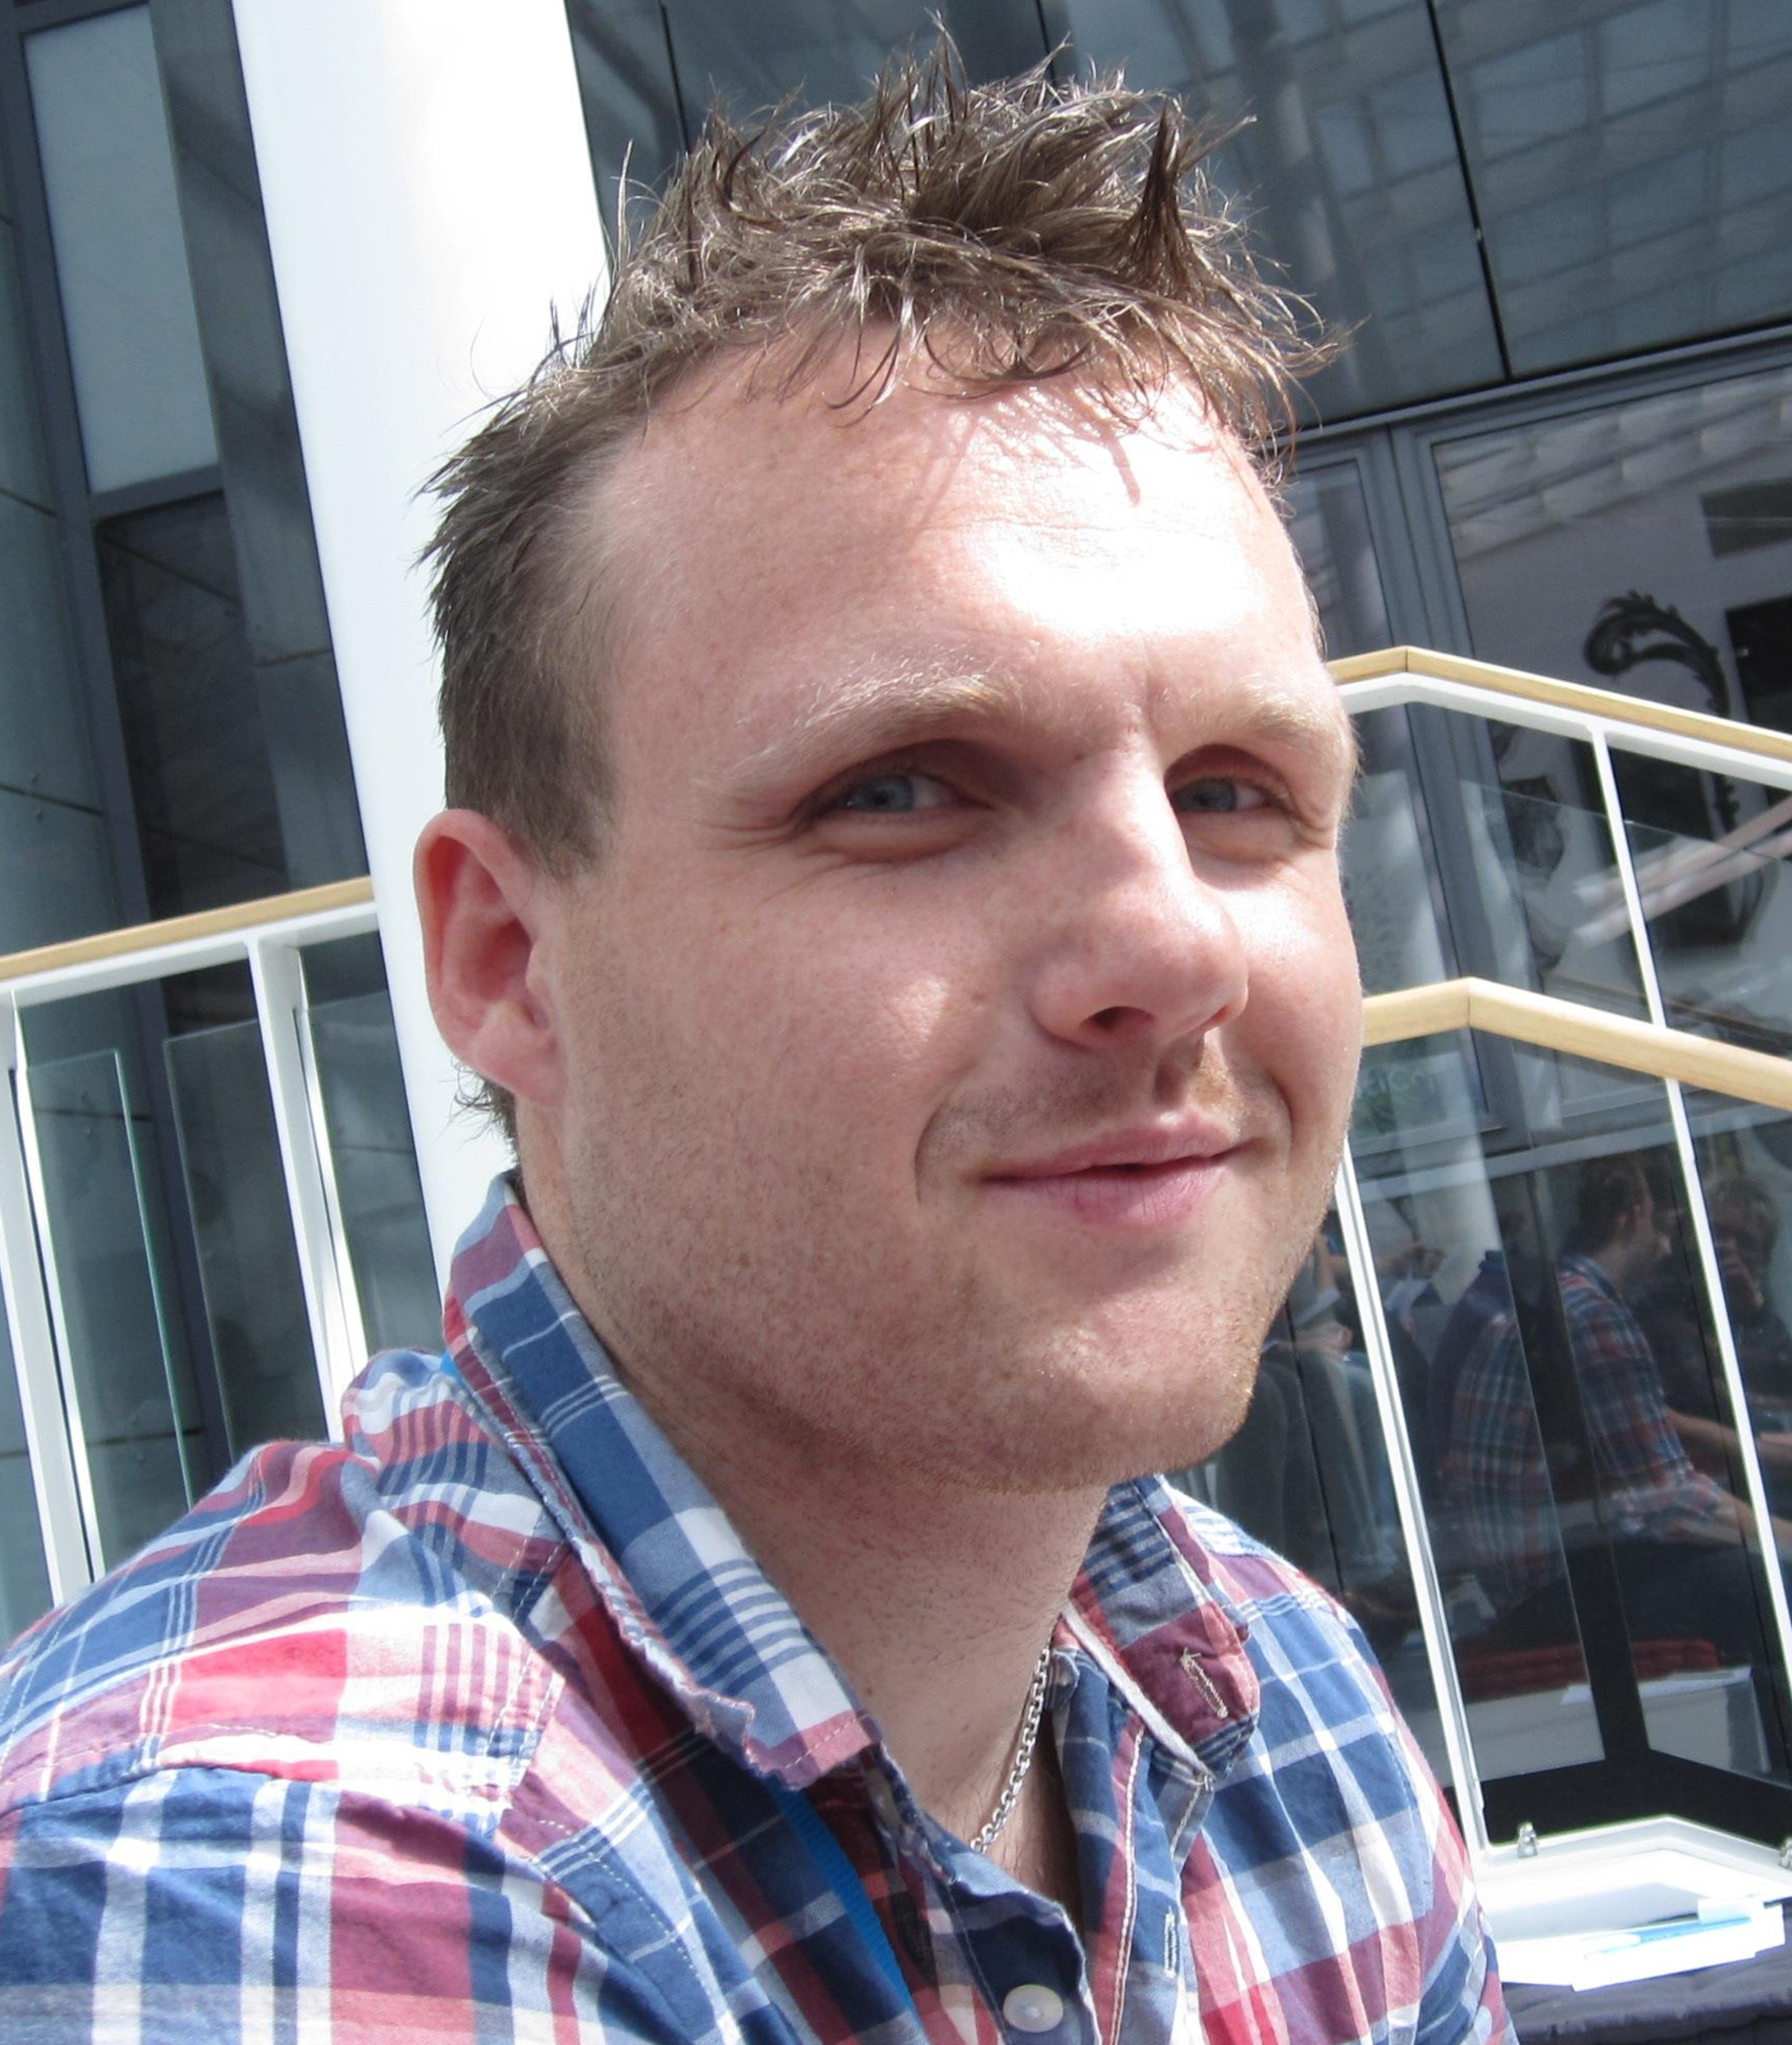
\includegraphics[width=0.52\textwidth]{IMG_3380.pdf}
\end{minipage}

\vspace{6mm}			
          
{\bf Supervisors:} \\
Prof. Rafa\l{} Wi\'{s}niewski\\
Postdoc. Kasper Vinther\\
Assist. Prof. Christoffer Sloth\\
Postdoc. Karl Damkj�r Hansen\\  
               
        
{\bf Existing copies:} 6\\
{\bf Pages:} 112 \\
{\bf Appendices:} 21 pages of appendices and \\
\textbf{Attached:} 1 CD \\\\

\vfill } &
      
\parbox{7cm}{
\vspace{2mm}
\hfill 
\begin{tabular}{l}
      {\bf Abstract:}\bigskip \\
      \fbox{
      \parbox{7cm}{\bigskip
            {\vfill{\small This will eventually become a synopsis.





 \bigskip}}
      }\hspace{0.2em}}
\end{tabular}}

\end{tabular}

\vspace{-3mm}
\hspace{2mm}
\parbox{18cm}{
\noindent\footnotesize\textit{
\begin{flushleft} 
	The content of this report is freely available, but publication (with source reference) may only take place by agreement with the authors.	
\end{flushleft}}}
    
}
\end{titlepage}
\input{formalia/tomside.tex}

\setcounter{page}{1}
\renewcommand{\thepage}{\Roman{page}}

%\newgeometry{left=4.5cm,top=-0.5cm,bottom=2cm,textheight=28cm,includefoot,textwidth=16cm}
\chapter*{Preface}
\vspace*{-2mm}
This report documents the development process of a safe controller for automation of a surgical robot arm with patient safety guaranteed through barrier certificates. %, preventing the robot tool from entering predefined unsafe regions. 
The access to robot measurement data and opportunity to implement a controller heavily benefits from the previous work carried out on the da Vinci surgical robot in the Control Laboratory at Aalborg University.
The project is rated at 30 ECTS-points, and the work is conducted by the 4$^\text{th}$ semester group 1032 within the graduate program in Control and Automation at Aalborg University during the spring of 2015.


%The target group is supervisors, students and other interested parties at the School of Information and Communication Technology at the The Faculty of Engineering and Science.

\vspace*{-2mm}
\section*{Reading Guide}
\vspace*{-2mm}
The primary focus of this report is to design a controller and a barrier certificate, the certificate guaranteeing the safe control of a surgical robot, as an approach to draw closer to the possibility of implementing automated control tasks by surgical robots. 
%Controllers and certificates are designed for static as well as dynamic boundaries of unsafe regions, such as e.g. a beating heart.
After an introduction into surgical robotics and the definition of barrier certificates, two approaches to the design problem are described:
\vspace*{-3mm}
\begin{itemize}
\itemsep-1.4mm
\item Explicit approach: A barrier certificate is constructed and a safe controller is designed according to the method described in \citep{bib:org_control}.
\item Analytic approach: A controller is designed, criteria are constructed for a barrier certificate and  safety is verified by use of Putinar's Positivstellensatz.
%\item \autoref{part:closure} Discussion \textcolor{red}{REWRITE!!!}
\end{itemize}
\vspace*{-2mm}

Symbols, acronyms and a glossary are presented in the nomenclature before the main report.
A variant of the Harvard referencing is used for citations, with the author and publication year of the source given in square brackets, e.g. [Lasserre 78], and sources listed in the bibliography at the end of the main report. % contains all references used in the report. Books are indicated with author, title, publisher, year and ISBN. Web pages are indicated with author, title and year.
%Chapters in the main report are numerally numbered while appendices are alphabetically numbered.
A comprehensive appendix is included after the bibliography, containing introductions to the used software, detailed derivations, measurement logs and source code.
A digital copy of this report along with cited references, source code and simulation results can be found on the enclosed CD.

\vspace*{-2mm}
\section*{Acknowledgements}
\vspace*{-2mm}
The authors wish to thank Assistant Engineer Simon Jensen for a thorough introduction to the custom made AAU da Vinci hardware and design of a dynamic heart phantom platform; Ph.D. Tobias Leth for guidance in reference frame construction for robot kinematics;  Post Doc. Karl Damkj\ae r Hansen for an introduction to the AAU da Vinci robot operative system and help in implementing inverse kinematics; and Assistant Professor Christoffer Sloth for help and guidance with the theory behind barrier certificates and the use of SOSTOOLS.

Last but not least, it is desired to thank chief surgeon Johan Poulsen, robot assistant nurse Jane Petersson and surgeon Grazvydas Tuckus for sharing their insights in the use of surgical robotics and allowing the attendance of a robotic surgery at Aalborg University Hospital.

%It is the wish of the authors to express a special appreciation to..

%\restoregeometry % efter denne side bruges de indstillinger der er sat i preamble
\input{formalia/tomside.tex}

\setlength\parskip{0ex}
\tableofcontents
\setlength\parskip{1ex}

\chapter*{Nomenclature}\label{chap:acronym}
\addcontentsline{toc}{chapter}{Nomenclature} % Adds chapter to TOC even though it is unnumbered
\printglossary[style=mcoltree,title=Glossary] %Print the glossary			%style=altlist
\printglossary[type=\acronymtype,style=glossary2col] %Print list of acronyms
\printglossary[type=symbols,style=altlong4col] %Print list of symbols
\clearpage

\section*{General Notation Remarks}
\vspace{0.1cm}

Vectors are written i bold upright lowercase letters e.g. \textbf{x}, and vector entries are written as the same italic lowercase letter with a subscript generally denoting its entry e.g. $x_1$. The composition of the entries will be clear from the context.
Matrices are written in bold upright uppercase letters e.g. \textbf{A}, its transpose is denoted by \textbf{A}$^T$ and its inverse  is denoted by \textbf{A}$^{-1}$.

The $n$-dimensional real Euclidian space is denoted by $\mathbb{R}^n$ and subsets of the real space are written in calligraphic letters e.g. $\mathcal{X}\subseteq \mathbb{R}^n$. 
A function is written in italic letters followed by the variable(s) it is a function of e.g. $f(\mathbf{x})$. A differentiable function defined on $\mathbb{R}^n$ is denoted by $f\in C^1(\mathbb{R})$.

The time derivative of a variable is indicated by a dot above the symbol e.g. $\dot{\mathbf{x}} = d\mathbf{x}(t)/dt$. In general the notation $(t)$ denoting a function of time is implicit for the state vector \textbf{x}, and is only included to emphasize the time dependency. For functions of the state e.g. $q(\mathbf{x})$  the notation $(\mathbf{x})$ is left out when the dependency is clear from the context. The derivative notation $dB(\mathbf{x})/d\mathbf{x}$ implies the row vector of partial derivatives of $B$ with respect to $x_1,...,x_n$. 

The function $B(\mathbf{x})$ should not be confused with the matrix \textbf{B}.









\textcolor{white}{%\gls{analytic_func} \gls{rational_func} \gls{proper_func} \gls{lipschitz} \gls{dimension} \gls{hurwitz} 
	\gls{injective_func} \gls{surjective_func} \gls{bijective_func}  \gls{compact_space}  \gls{extrinsic} \gls{intrinsic} \gls{tcp} \gls{Ts} \gls{y} \gls{radius_vec} \gls{center_vec}}

\cleardoublepage
\setcounter{page}{1}
\renewcommand{\thepage}{\arabic{page}}

\chapter{Introduction}\label{chap:intro}
\vspace{-3mm}
When the recovery from an injury or disease requires a surgical procedure, traditionally this has been done with open surgery, where the patient is cut open for the surgeon to perform the procedure. For many types of operation, however, alternatives to open surgery have emerged, especially over the last half century.
In \gls{mis}, as opposed to traditional open surgery, only small incisions are made in the patient's abdomen or pelvis in order to gain access to the area under surgery, hence causing less trauma beyond this confined area. This in general provides the patient with quicker recovery, shorter hospital stay and less scarring.
One type of \gls{mis} is \gls{laparoscopy}, invented in the beginning of the 20th century \citep{bib:laparoscopy}, where thin metal telescopes (laparoscopes) with specialized surgical tools attached are inserted into the patient through trocars, allowing the surgeon to maneuver the tools in the inflated abdomen guided by visual feedback from a flexible miniature camera (\gls{endoscope}) inserted alongside the surgical tools \citep{bib:fascrs}, see \autoref{fig:laparoscopy}.
In the 1980s robotic laparoscopic surgery was introduced as a master-slave system, where the surgeon controls a robot arm holding the surgical tools from a master console, instead of manipulating the instruments manually.

\vspace*{3mm}
\begin{figure}[htbp]
\centering
\begin{minipage}{0.39\textwidth}
\subbottom[Manual laparoscopic tools.]{\includegraphics[width=\textwidth]{laparoscopic_instruments_manual_red.jpg}\label{fig:laparoscopic_instruments_manual}}%
\vspace*{3mm}
\subbottom[Robotic laparoscopic tools.]{\includegraphics[width=\textwidth]{laparoscopy_20150312_134752.jpg}\label{fig:laparoscopy_20150312_134752}}%
\end{minipage}
\hspace*{5mm}
\begin{minipage}{0.258\textwidth}
\subbottom[Tool in trocar.]{\includegraphics[width=\textwidth]{laparoscope_20150317_111908_red.jpg}\label{fig:laparoscope_20150317_111908}}%
\end{minipage}
\hspace*{5mm}
\begin{minipage}{0.258\textwidth}
\subbottom[Endoscope.]{\includegraphics[width=\textwidth]{endoscope_20150430_124054.jpg}\label{fig:endoscope_20150430_124054}}%
\end{minipage}
\caption{Tools used in laparoscopic surgery.}
\label{fig:laparoscopy}
\end{figure}

\section{Highlights in the Development of Surgical Robotics}

\vspace{-1mm}
While the idea of roboticized telemedicine dates back to 1925 \citep{bib:telemed_predict}, the development of telesurgery was founded by the \gls{nasa} in the 1970s %\citep{bib:telesurg_history} 
combining research within virtual reality, robotics and medicine, %\citep{bib:brown_univ}, 
and the first robotic surgery procedure was accomplished in 1985, %\citep{bib:telesurg_history}, 
followed by the first laparoscopic robotic surgical procedure in 1987 \citep{bib:telesurg_history,bib:brown_univ}.
In 1998 the first fully endoscopic robotic surgery were performed and the idea of operating on a beating-heart were initiated \citep{bib:brown_univ}. 
%endoscopic coronary bypass procedure were performed \citep{bib:brown_univ}.


%The first commercially available surgical robot ROBODOC (from Curexo) was introduced and performed the first robotic joint replacement surgery in 1992, and in 1994 the AESOP (from Computer Motion) was the first robotic system approved by the \gls{fda} for general surgery \citep[p 74]{bib:telesurg_history,bib:surgical_book}.

The first commercially available surgical robot was introduced in the early 1990s. At the same time major research within telesurgery was funded by \gls{darpa}, %and two main teleoperation systems were developed from this research: da Vinci (from Intuitive Surgical) and Zeus (from Computer Motion) \citep{bib:telesurg_history}.
concurrent with the U.S. Army developing the \gls{mash} for loading and teleoperating wounded soldiers in vehicular operating rooms \citep{bib:telesurg_history,bib:brown_univ}.

%In the early 1990s the U.S. Army developed \gls{mash} for loading and teleoperating wounded soldiers in vehicular operating rooms \citep{bib:brown_univ}, and in 1993 the idea for a robotic slave manipulator arm was conceived by Madhani after watching an episode of the tv-show M*A*S*H [SurgRob], and he created the Black Falcon during his work at MIT \citep{bib:black_falcon} later becoming he prototype of the da Vinci arms.

Surgical robots teleoperated from more than a few meters away is, however, still incipient. In 1996 the first tests were performed demonstrating the successful use of telementoring and telemanipulation of the endoscope by a surgeon placed several 100\,m away from the operating room, % \citep{bib:telesurg_history}. 
%In the late 1990s \gls{nasa} and \gls{darpa} sponsored research within light-weight and deployable space surgical robotics for remote teleoperation, resulting in two main robotic systems: the Raven (from University of Washington) and M7 (from SRI International) [SurgRob].
%
%and in 2000 da Vinci (from Intuitive Surgical) became the first robotic surgical system  to be approved by the \gls{fda} for general laparoscopic surgery \citep{bib:mddi}.
%
and in 2001 the first transatlantic telesurgical procedure, the Lindbergh Operation, was performed by a team of French doctors in New York %manipulating the arms of a Zeus robot to perform a gall bladder 
operating on a patient in Strasbourg \citep{bib:telesurg_history}. More research into remotely telementored and teleoperated robotic surgery was performed during the 2000s with the NASA Extreme Environment Mission Operations (NEEMO) projects  %in the Aquarius undersea lab in Florida %, in 2003 with Zeus controlled from Ontario 2500 km away \citep[pp 75, 81]{bib:surgical_book} and in 2006 and 2007 with Raven and M7 controlled from Seattle \citep[pp 28, 82]{bib:surgical_book}. 
%
and as part of the \gls{darpa} Trauma Pod program launched in 2005 \citep{bib:surgical_book,bib:docatadist}.

%In 2005 \gls{darpa} launched the Trauma Pod program for developing an unmanned autonomous and semi-autonomous mobile military operation platform, funding research for e.g. SRI and for the Raven project. The goal of the first phase of the project was achieved in 2007 with the successful demonstration of a prototype trauma pod consisting of a da Vinci robot, a \gls{mash} stretcher and a custom nurse robot \citep[p 30]{bib:surgical_book}. The second phase aims at miniaturizing and integrating the systems \citep[p 31]{bib:surgical_book}, and in 2005 a demonstration was performed by roboticists, surgeons, aerospace engineers and networking experts in the desert placing the Raven patient manipulator and the controller console 100 m apart and relaying the communication link via a drone \citep{bib:docatadist}.



%In 2006 the first-ever demonstration of unmanned telesurgery with M7 [SurgRob]
%
%M7 performed the world's first automated ultrasound guided tumor biopsy in 2007 [SurgRob]
%
%2008 neuroArm was first used to remove a brain tumor [SurgRob]

%\gls{nasa}'s first experiment in a zero gravity environment was performed with an acceleration compensated M7 in 2007 on a parabolic flight \citep[pp 29, 76, 85]{bib:surgical_book}, and in 2011 \gls{nasa} sent the humanoid robot Robonaut 2 to \gls{iss}, and it has since been trained in telemedicine [SurgRob].







\section{State-of-the-Art in Surgical Robotics}

\vspace{-1mm}
Most surgical robots used for telesurgery are master-slave systems which can be fully controlled by the surgeon, see \autoref{fig:master-slave_surgery}. % \citep{bib:raven_debride}. 
The patient manipulator consists of 2-4 robotic arms, each having 6-7 \gls{dof} % \citep{bib:raven_debride} 
including the arm, wrist and the end effector (the tip of the laparoscopic tool), one of the arms holding a stereo-vision \gls{endoscope} \citep{bib:raven_debride}. 
The end effectors are positioned by high-precision motors and are able to reach spaces a human hand cannot \citep{bib:docatadist}, and furthermore development is progressing within flexible end effector tools \citep[p 74]{bib:surgical_book}. %, but even microrobots entering the body through natural orifices and controlled via electromagnetic fields or nanosensors and -actuators are being developed [SurgRob].

\vspace{-3mm}
\begin{figure}[htbp]
\hspace*{-5mm}
\subbottom[Surgeon master console and slave robotic patient manipulator.]{\includegraphics[width=0.5\pdfpagewidth]{davinci_surgical_system.jpg}\label{fig:davinci_surgical_system}}%
\subbottom[The robotic patient manipulator.]{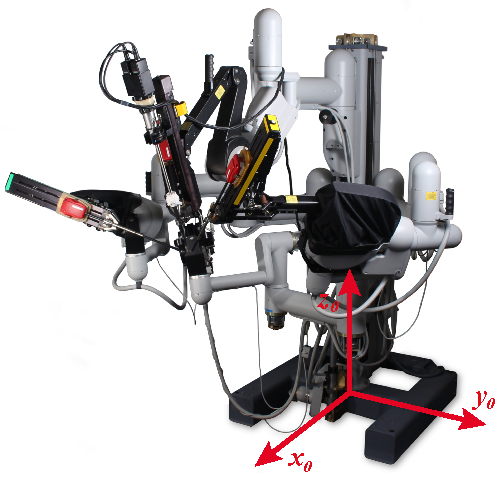
\includegraphics[width=0.4\textwidth]{robot_base_frame1.jpg}\label{fig:robot_base_frame}}%
\caption{Example of a master-slave robotic surgical system: the da Vinci.}
\label{fig:master-slave_surgery}
\end{figure}

The 3D visual feedback from the endoscope is sent to the master console, % which can have eye-tracking for adaptive field of view and safety stop if the surgeon's gaze is not fixed at the operation site [SurgRob]. The 
and the control signals for the surgical instrument are generated with the controller joystick, which scales the surgeon's movements down to micro-movements \citep{bib:intuitive_monopoly} steerable through the (zoomed) 3D visual feedback. It also filters away tremor, and development is made within haptic feedback to the joystick \citep[p 89]{bib:surgical_book}, enhancing the surgeon's feel, enabling greater dexterity, accuracy and stability than a human hand.

In the first generations of surgical robotics the master and slave had to be in the same room, %(as is the case with da Vinci) \citep{bib:telesurg_history,bib:raven_debride,bib:surgical_book},
but although the feasibility of conducting surgical interventions remotely has been demonstrated, there has not been drivers strong enough to justify its implementation \citep[p 38]{bib:surgical_book}. Experiments and development are made within minimizing and coping with the delays for long-distance telesurgery and within miniaturization and robustness of the surgical robotic systems for use in harsh environments such as war and space. %, e.g. for da Vinci's potentially closest competitor, the open-source Raven.

Robotic surgical procedures are beginning to show superiority to conventional surgery for some procedures, but is still considerably more expensive \citep{bib:docatadist}. 
The excessive price  is particularly owed to Intuitive Surgical's many patents securing Intuitive the predominant market share with more than 3000 da Vinci Surgical System units installed worldwide (of which 70\,\% are in the U.S.) \citep{bib:intuitive_monopoly}.
%In some cases robotic procedures are faster than conventional surgeon procedures [SurgRob], but still in other it is much slower \citep{bib:raven_ii,bib:raven_debride}.
Autonomous procedures are still only implemented for entirely pre-planned motions of an operation, and depending on the type of operation not all subtasks in an operation are suited for autonomy \citep{bib:raven_debride,bib:raven_ii}.


%\textcolor{red}{New generation: surgical care not only to soldiers but also to remote locations lacking specialized physicians. - better tactile feedback because the surgeon needs to feel the tissue and the difference in its stiffness}


 
%\subsection{The da Vinci Surgical System}
%Although several \gls{fda} approved robotic surgical systems exist, da Vinci is still the only commercially available system \citep{bib:docatadist,bib:intuitive_monopoly}. 
%The first da Vinci prototype was developed at SRI under contract with the U.S. Army in the late 1980s \citep{bib:mddi,bib:brown_univ}, and in the early 1990s \gls{darpa} invested in the research \citep[p 74]{bib:surgical_book}. In % the mid 1990s SRI licensed the manipulator design of Madhani along with many other patents, and in 
%1995 SRI founded Intuitive Surgical and the focus shifted from battlefield to commercial use in hospitals \citep{bib:intuitive_monopoly}.
%In 1997 the first human trials were performed \citep{bib:intuitive_monopoly} %, in 1999 the first market-ready da Vinci began tests [SurgRob] 
%and the system was first approved by the FDA in 2000 \citep{bib:intuitive_monopoly,bib:brown_univ}. From 2000 until the merger in 2003 Intuitive Surgical and Computer Motion had a number of lengthy patent litigations \citep{bib:intuitive_monopoly,bib:telesurg_history}.





%The da Vinci Surgical System still has the predominant market share with more than 3000 units installed worldwide due to being the first-mover in the field and due to their many patents \citep{bib:intuitive_monopoly}, and has only had one serious case of a patient dying after surgery (2002) [SurgRob].
%The expiration of their patents in 2015 and 2016 \citep{bib:intuitive_monopoly} shows promise of many other robotic surgery systems entering the market, as both American, Canadian, European and not least Asian similar systems exist that are considerably cheaper than the da Vinci, and also more lightweight.

%In 2013 Intuitive released the da Vinci Research Kit platform, built from mechanical components from first generation da Vinci (two arms and a surgeon console), open-source electronics and university-developed software \citep{bib:raven_observ}.

%\subsection{The Raven Surgical Robot}
%One potential challenger to da Vinci is the Raven \cite{bib:mddi}, an light-weight open-architecture 2-armed surgical robot \citep{bib:raven_debride,bib:raven_ii} originally developed by University of Washington funded by multiple U.S. government agencies including the Army and the \gls{dod} \citep[p 27]{bib:surgical_book}.
%Raven-II is installed at 10 different universities in the U.S. and one in France \citep{bib:raven_ii}, sharing research innovations and using open-source software (including the ROS middleware) to create surgery subtasks \citep{bib:raven_debride}. 
%As Intuitive Surgical's patents gradually expire the University of Washington is considering the possibility of spinning off the Raven into a start-up company \citep{bib:economist}.
%
%The Raven robot is focused on remote telesurgery (with notable latency) in harsh conditions \citep{bib:docatadist}, and research at University of California has been made in teaching a computer model to autonomously mimic laparoscopic surgeons from recordings dynamic and kinematic data of their motions in a multi-state statistical Hidden Markov Model \citep{bib:economist}. 
%The primary difficulty reported from controlling the Raven has been state estimation, necessary because of the uncertainty inherent in actuators and encoders connected to flexible elements via long cables \citep{bib:raven_debride} and the necessity of collision avoidance of the arms.

\section[Envisioned Future for Robotic Surgery at Aalborg University Hospital]{Envisioned\,Future\,for\,Robotic\,Surgery\,at\,Aalborg\,University\,Hospital}\label{sec:aau_doc}

At Aalborg University Hospital robotisized \gls{mis} has been implemented since 2008, and now count two da Vinci surgical robots employed at the urology and gynaecological wards, each performing 230 surgeries a year. %(og en i dyrelaboratoriet til at øve på)
Johan Poulsen, chief surgeon at the urology ward and manager of the Center for Minimally Invasive Surgery at Aalborg Univeristy Hospital, concurs with the stance that robotic laparoscopy provides the surgeon with greater dexterity, stability and precision due to the design of the robot tools, the tremor filtering, micro-movement down-scaling %of approx 10-15 times
and 3D visual overview of the surgical site.  %a 2D camera used in manual laparoscopy.
It also allows the surgeon a much better work posture than manual laparoscopic surgery and he argues that it is easier to learn operating the robot than manual laparoscopic tools, %not least for the suturing technique, 
and with the generations now entering the job market mastering  robotic technologies for surgery will come naturally.


At present the da Vinci robot is routinely used in Denmark in procedures within gastroenterology, gynaecology and urology. Dr. Poulsen, who is one of the nationally leading experts within robotic surgery, argues that the next few years will also see robotics applied in surgery of the alimentary tract as well as in otorhinolaryngological, lung and heart surgery, in pace with the purchase and maintenance price of surgical robots going down.

According to Dr. Poulsen one of the greatest challenges in operating on a beating heart is the concluding part of the operation suturing the operation site, as the moving tissue is easily pinched or tugged. 
In order for the advantages of robotisized heart surgery to compensate for the drawbacks of manual bypass operations, it is paramount to have a very exact model of the heart movement. 
As the heart movement is not a beat as such but rather an expansion and contraction movement propagating from one end of the heart to the other, even a highly complex model will need correction from position measurements of the surface of the heart. 
He sees it as a viable possibility to mount sensors of up to two by two centimetres by sowing them to the surface of the heart and having a tracking system such as e.g. the Vicon system (Vicon is an indoor tracking system similar to the outdoor GPS) being part of the range of surgical instruments in order to get extremely exact position data for the motion-compensated surgical robot.


Dr. Johan Poulsen suggests a surface mounted on a cylinder, which can be controlled to periodically move up and down, as a first step in testing a surgical robot in following the movement of a surface.





%så ser han den også blive brugt indenfor mave/tarm, øre/næse/hals, mikrokirurgi, hjerte, lunge, og mener bestemt det er fremtiden



%Forhindringer
%
%The cost price of 15 million DKK is too high (Johan Poulsen)
%
%fremtid: folk skal kunne se fordelen ved at bruge den i forskellige typer af operationer, men det er meget prisen der sætter begrænsningen, Intuitive holder prisen utroligt højt oppe, indkøbspris ca 25 mio kr, plus årlig service på 2.5 mio kr, plus 1600-1500 kr pr instrument som kun kan bruges 10 gange. Johan Poulsen vurderer at det skal ned i 1/5 pris for at det kommer ind på mange andre områder, 
%
%
%
\section{Establishment of Da Vinci at Aalborg University}\label{sec:technical_overview}
%A surgery consists of a series of subtasks, some suited for robotized autonomous execution. Prior work in motion planning and control of subtasks for surgical robots include knot tying, suturing and more advanced statistical learning of subtasks from recording surgeon motions \citep{bib:raven_debride,bib:raven_observ}.
%
The configuration at Aalborg University is based on a first generation Da Vinci surgical robot, detached from its surgeon controller console and modified to be controllable by automated processes. The setup is physically located at the Control and Automation laboratory at Aalborg University. Before a technical overview of the system is given in \autoref{sec:technical_overview}, an overview of used terminology is outlined in \autoref{fig:naming_convention}.
\begin{figure}[H]
\centering
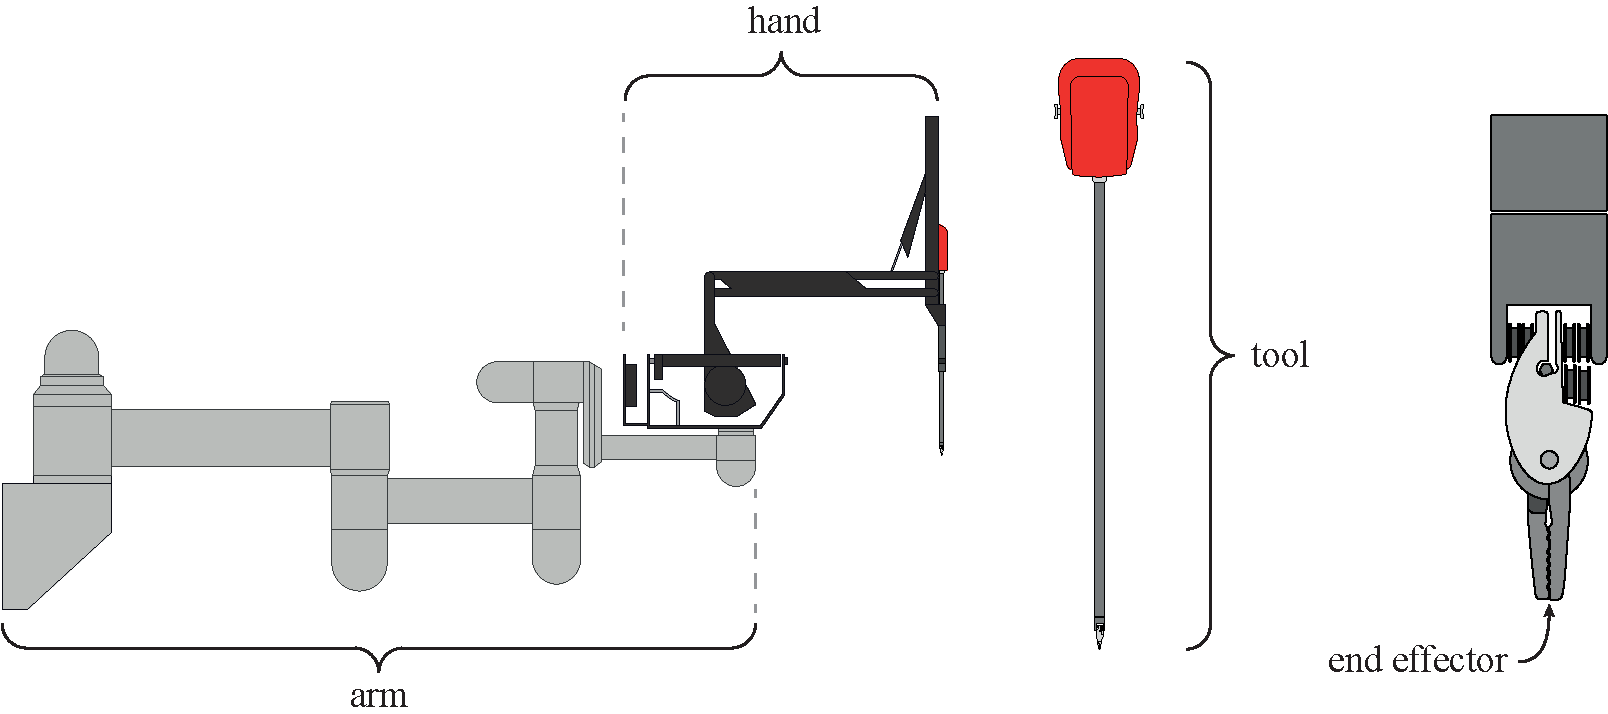
\includegraphics[width=1\textwidth]{naming_convention.pdf}
\caption{Naming convention used for the da Vinci robot.}
\label{fig:naming_convention}
\end{figure}
\Autoref{fig:naming_convention} depicts the distinction of the robotic parts such that the far left part is named the "arm" which is uncontrollable (but adjustable). The center left part consists of the controllable dynamic parts which is labelled as the "hand". The "tool" located center right consists of a replaceable instrument worth 10.000\,kr and only certified to be used for 10 operations. The outermost part of the instrument is labelled the "end-effector" and it is  this which should follow a reference point in the developed controllers.

%
%\subsection{Technical Overview of the Robotic Surgery System}
%A simplified overview of the robot controller setup is provided in \autoref{fig:overview}. 
%
The technical overview in \autoref{fig:overview} is structured in descending abstraction layers with the highest at the top (i.e. the \gls{ros} - an open source software framework for robots \citep{bib:ros}, see \autoref{app:ros} for further details), which establishes a wireless TCP/IP communication channel receiving all positions from the robot as feedback and produces position control signals to the NI (National Instruments) single board \glspl{rio} which handle all input/output communication with the user. The NI single board \glspl{rio} consist of a primary and a secondary board. The reason for having two \gls{rio} boards is solely the lack of input/outputs on one board.

The \gls{rio} boards direct the control signals to a cascaded controller taking in a position reference from the user and delivering a current control signal to the ESCON motor driver. The velocity and current controllers are implemented in \gls{fpga} based hardware to ensure sufficient controller speed relative to the system \citep{bib:robot_paper}. The ESCON motor driver manages advanced processing and essentially delivers an appropriate PWM signal for the actuators (seven Maxon motors) which represent the lowest abstraction layer, located at the bottom of the figure.

The NI single board \glspl{rio} concurrently handle most safety precautions and enabling/disabling movement of the arm itself (see \autoref{app:links_joints_3d} and \ref{app:kinematic_model_robot} for an overview of the arm and its kinematics, respectively) through solenoids.
\begin{figure}[H]
\hspace*{-5mm}
\includegraphics[width=1.1\textwidth]{overview.pdf}	
\caption{Overview of the custom made hardware and controllers for the 1st generation da Vinci surgical robot located at Aalborg University's department of Control and Automation.}
\label{fig:overview}
\end{figure}

In order to prevent potential violation of physical joint constraints, stricter constraints on each joint position are set in the low-level motor controllers, that disable the controller if exceeded.

An introduction to the Da Vinci system has at this point be given. Thus the contribution of this project will be outlined in the upcoming subsection.

{\color{red}{The robotic patient manipulator constitutes four "arms" (see \autoref{fig:master-slave_surgery}) each comprising a number of arm links, whose joints are fixed by electromagnets that are manually released for positioning of these links; followed by the robot "hand" and instrument links, whose joints are available for automated control on the modified AAU da Vinci robot. Only the controllable part of the robotic patient manipulator, as displayed in \autoref{fig:robot_hand_3d}, is considered in the design of the 3D Cartesian space controller. }}
\subsection{Overview of Thesis Contribution to the AAU da Vinci System}\label{sec:project_overview}
The focus of this thesis is the highest abstraction layer as seen in the top of \autoref{fig:overview}, i.e. the ROS environment. The purpose of this layer primarily constitutes the implementation of algorithms that require heavy processing and non real-time processing or tasks with loose timing constraints \citep{bib:robot_paper}.
Given the topics described in the introduction to this project and the desire to automate surgery by means of the Da Vinci robot, this thesis will practically and theoretically encompass the tasks outlined in \autoref{tab:requirement}.
\begin{table}[H]
\begin{tabularx}{\textwidth}{X X}
\rowcolor{HeaderBlue} 
\textbf{Problem} &  \textbf{Origin}\\
Design a position controller such that it is possible to specify regions where it can be guaranteed that the end-effector will never enter. & Provide the surgeon with a feature ensuring that certain regions will never be touched, e.g. veins and similar. \\
\rowcolor{textBlue} 
Design a position controller taking  user input relative to a point on the surface of a beating heart while ensuring that the heart is not penetrated. & Founding automated control on beating hearts where a safe distance to the heart is maintained such that the heart under no circumstances is penetrated.\\
Modelling the system sufficiently without touching the underlying controllers & The cascaded controllers seen in \autoref{fig:overview} are not to be touched. Safety is desired solely from the ROS environment. \\
\rowcolor{textBlue} 
Implement the controllers physically on the Da Vinci Robot. This also implies an understanding of the entire \gls{ros} framework & Verify the theory in practice and thereby be a first mover on this topic \\
\end{tabularx}
	\caption{Problems to be solved throughout this thesis and why they are desired to be solved.}
\label{tab:requirement}
\end{table}
The problems given in \autoref{tab:requirement} may be solved in a number of ways and it is not initially obvious which is the more appropriate one. For that reason, it is chosen to bifurcate a solution strategy, thus two approaches are used:
\begin{itemize}
\item The design of a safe end-effector setpoint controller, utilizing a control barrier functions such that the robot is physically prevented from entering unsafe areas thereby guaranteeing safety in real time \citep{bib:safety}. 
\item The design of a controller unrestricted from safety considerations. The safety is ensured before the controller is physically implemented by conducting an analysis adjudicating the safety. Thus the controller well be given a \textit{pass} verdict if it does not violate the safety conditions and a \textit{not pass} verdict if it violates predefined safety conditions which suggest an iteration of the controller such that it becomes safe. 
\end{itemize}
Th analysis of these two strategies ought to give an indicator for which method may be the most appropriate one to use given a specific problem and its complexity taken into account. Consequently, this report presents algorithms, analysis, controllers, software development and formal verification that guarantees safety for automated surgeries.

The chapters in this report are split such that a certificate to guarantee the safety is established in \autoref{chap:barrier_cerificates} followed by \autoref{chap:cbf} where the applied theory to design a controller that guarantees safety for specified regions is described. Thus \autoref{chap:cbf_1d_static} provides an exhaustive example of how to apply the theory to the Da Vinci robot. \Autoref{chap:cbf_1d_dynamic} concerns safety while operating on a beating heart. Next is \autoref{chap:cbf_3d_static} which founds safety in the three dimensional space. An interim conclusion is given in \autoref{chap:interim} which concludes the need for an easier way to construct the certificates. Thus \autoref{chap:putinar} describes a way to apply automated software which ought to ease the search for certificates. Thereby, \autoref{chap:sostools} provides examples of how to apply the software to the use-cases described in the preceding chapters. \textcolor{red}{Finally, chapter ?? concludes...}



%Raven-II inverse control process (not primarily to estimate the pose, in which case standard estimation methods like Kalman would be appropriate) is to calculate, give an desired true pose, the input pose to send the control sw to reach the desired true pose (detected pose with vision system assumed to be the true pose), estimate between measurements using updates from forward kinematics \citep{bib:raven_debride}.

%advances in motion planning, control and perception: integrated task and motion planning ofhigh level task planning using state machines, and motion planning for low level planning algorithm  \citep{bib:raven_debride}

%da Vinci Research Kit: learning from demonstrations/by observation. Targets considered form convex regions spherical/linear. \citep{bib:raven_observ}.

\chapter{Safety Guarantee by Barrier Certificates}\label{chap:barrier_cerificates}
	A crucial matter when designing a controller for automated operation of robotic surgery tools is the necessity of guaranteed patient safety. The system has to not only be able to prevent the surgery tool from entering certain regions, e.g. penetrating the wall of the heart or cutting an artery, but to guarantee that this cannot happen under any circumstances.


Casting the controller design problem as an optimization problem with constraints, such as \gls{mpc}, could in principle guarantee that the tool would not enter a predefined area. Indeed, \gls{mpc} is a method which is very popular at the higher abstraction layers, such as setpoint control \citep{bib:mpc_simon} which is the case in this specific study. However, most solvers such as the Matlab plugin \texttt{cvx} requires convexity in the performance function and its constraints to be able to find a global minimum. This will at best be a lucky special case that unsafe regions can be defined through a convex function.  
Furthermore, \gls{mpc} is mostly used in systems with slow dynamics, i.e. dynamics where the time constant is measured in seconds or even minutes \citep{bib:mpc_slow}. This is obviously due to heavy online computations and numerous iterations. Systems containing these time constants are usually thermal systems and not mechanical systems. Additionally, the feasibility of the optimization problem is not very transparent and it is well known that \texttt{cvx} is very likely to crash due to infeasibility.
%, but a hard constraint would fail to follow the dynamics of a moving area boundary such as a beating heart. 

Another very elegant and computationally efficient approach to the safe controller analysis and design problem is the use of barrier certificates, which provide a formal proof of safe operation in infinite time horizon \citep{bib:prajna_framework,bib:safety}. This chapter describes the requirements for the construction of barrier certificates along with notation used in relation to these.
%


%dealing with those topics within robotic surgeries feature necessary conditions to guarantee the patient safety and to avert patient trauma .



\section{Constraints for a Barrier Certificate}\label{sec:safety-def}

When a barrier certificate can be found for a (closed-loop) dynamical system, the controller is guaranteed to be safe. In the following the notion of safety is defined in order to describe the guarantee extent of a barrier certificate. A general state-space representation of an $n$-dimensional non-linear system is considered:
\begin{equation}
\dot{x} = f_{cl}(x) + h(x)\,d = f(x) + g(x)\,u + h(x)\,d
\label{eq:general_statespace}
\end{equation}
\begin{tabular}{rl} 
where &  \\
\gls{x} &  is the state, $x(t) \in \mathbb{R}^n$\\
\gls{u} & is the control input, $u(t) \in \mathbb{R}^m$\\
\gls{d} & is the disturbance input, $d(t) \in D \subseteq \mathbb{R}^p$ \\
\gls{f} & is a non-linear function, $f:\mathbb{R}^n \rightarrow \mathbb{R}^n$\\
\gls{g} & is a non-linear function, $g:\mathbb{R}^n \rightarrow \mathbb{R}^{n \times m}$\\
\gls{h} & is a non-linear function, $h:\mathbb{R}^n \rightarrow \mathbb{R}^{n \times p}$
\end{tabular}\\

Consider a subspace of the state-space $\mathcal{X}\subseteq\mathbb{R}^n$ defining e.g. the physically feasible states for the system in \autoref{eq:general_statespace}. Within this region $\mathcal{X}$, define the two non-intersecting subspaces $\mathcal{X}_u\subset\mathcal{X}$ and $\mathcal{X}_0\subseteq\mathcal{X}$, defining an unsafe  and a safe region, respectively. The unsafe region contains the states which the trajectory of the system must never enter, e.g. for a surgical robot this space could be the collection of veins and organs near the operation site, for which perforation is prohibited. The safe region contains all the states which the trajectory of the system is allowed to and may be required to enter, e.g. the operation site and a region for entering the area in the abdomen.
Now safety of a closed-loop control system is given according to \citep{bib:safety,bib:prajna_framework} as:
%\begin{exa}

\begin{defn}[Safety of a System]\label{def:safety}
Denote a trajectory starting in $x(0)=x_0$ and with bounded disturbance function $\bar{d}:\mathbb{R}_{\geq 0}\rightarrow D$ by $\phi_{x_0}^{\bar{d}}$, defined by 
\begin{equation}
\frac{d \phi_{x_0}^{\bar{d}} }{dt} = f_{cl}\left( \phi_{x_0}^{\bar{d}} (t) \right) + h\left( \phi_{x_0}^{\bar{d}} (t) \right) \bar{d}(t)
\end{equation}
The system $\Gamma_{cl} = (f_{cl},h,\mathcal{X},\mathcal{X}_0,\mathcal{X}_u,D)$ is unsafe if there exists a $t \in [0,$\gls{T}$]$ such that the trajectory $\phi_{\mathcal{X}_0}^{\bar{d}}:\,[0,T]\rightarrow \mathbb{R}^n$ with initial state $x_0\in \mathcal{X}_0$ and bounded disturbance function $\bar{d}$ satisfies
\begin{flalign}
\left( \phi_{\mathcal{X}_0}^{\bar{d}}([0,t]) \cap \mathcal{X}_u \right) \neq \emptyset \kk \text{and} \kk 
\phi_{\mathcal{X}_0}^{\bar{d}}([0,t]) \subseteq \mathcal{X}
\label{eq:defsafety}
\end{flalign}
\noindent
The system $\Gamma_{cl}$ is safe if there are no unsafe trajectories.
\end{defn}

%\vspace{-0.2cm}
%
%\begin{longtable}{p{.9\textwidth} p{.1\textwidth} p{.1\textwidth}} 
%Where  & & \\
%\gls{fcl} is a potential non-linear function with the closed loop characteristic:\\ \kk $f_\text{cl}: x \mapsto f(x)+g(x)k(x)$ where \gls{k} is the feedback gain with the map $k: \mathbb{R}^n \rightarrow \mathbb{R}^m$ & [$\cdot$] &  \\
%\gls{X} is the set of all allowed states & [$\cdot$] &  \\
%\gls{X0} is the set of all allowed initial states & [$\cdot$] &  \\
%\gls{Xu} is the set of all unsafe states & [$\cdot$] &  \\
%\gls{phi} is the set of all allowed initial conditions with the bounded disturbance input \gls{dbar} & [$\cdot$]
%\end{longtable}

A graphical interpretation of \autoref{eq:defsafety} is shown in \autoref{fig:defsafety}.

\begin{figure}[H]
	\center
	\includegraphics[width=0.6\textwidth]{safety.pdf}	
	\caption{Graphical interpretation of \autoref{eq:defsafety} in the state space. The blue trajectory is unsafe because $\left( \phi_{\mathcal{X}_0}^{\bar{d}}([0,t]) \cap \mathcal{X}_u \right) \neq \emptyset$, while the green trajectory is safe.}
	\label{fig:defsafety}
\end{figure}
%\end{exa}

Disturbances are not considered in the scope of this project, and hence $d\in D$ is considered to be zero in the remainder of this thesis.

For the system in \autoref{eq:general_statespace} safety can be guaranteed if a barrier certificate for the system exists. A barrier certificate is defined as a function of the system state, satisfying a set of inequalities, entailing that its zero level set in the state space forms a barrier between the safe set of initial states $\mathcal{X}_0$ and the unsafe set $\mathcal{X}_u$, thereby certifying system safety \citep{bib:prajna_framework}.


If a barrier certificate can be defined, safety can be guaranteed for the closed-loop system in the region $\mathcal{X}$, with unsafe region $\mathcal{X}_u$, defined by positive values of the barrier function, and (safe) initial region $\mathcal{X}_0$, defined by non-positive values of the barrier function. In the below the notation $L_{f_{cl}}B(x)$ denotes the Lie derivative of \gls{bar} along the vector field of the closed-loop system $f_{cl}(x)$, corresponding to the time derivative of the barrier function i.e.
\begin{equation}
L_{f_{cl}}B(x)=\frac{dB(x)}{dx}f_{cl}(x)=\frac{dB(x)}{dx}\frac{dx(t)}{dt}=\frac{dB(x(t))}{dt}
\end{equation}

Requiring that the time derivative of the barrier function must be nonpositive on the entire set $\mathcal{X}$ (see \autoref{def:barrier_certificate}) corresponds to the value of the barrier function decreasing over time, hence seeking the minimum of the (convex) barrier certificate. Requiring the trajectory of the state to start within the safe set $\mathcal{X}_0$ this means that the trajectory will never cross the zero level set and enter the unsafe set $\mathcal{X}_u$, as this set only contains values of the barrier function larger than the initial value.

\begin{defn}[Barrier Certificate]\label{def:barrier_certificate}	
If a barrier certificate can be constructed as a continuous and differentiable function $B(x):\mathcal{X} \rightarrow \mathbb{R}$ adhering to the following inequalities  \citep{bib:prajna_framework}:
\begin{subequations}\label{eq:barrier_constraints}
\begin{flalign}
B(x) &\leq 0 \kk  \forall \hspace{2mm} x \in \mathcal{X}_0  \label{cer1}\\
B(x) &> 0  \kk  \forall \hspace{2mm} x \in \mathcal{X}_u \label{cer2} \\
L_{f_{cl}}B(x) &\leq 0 \kk  \forall \hspace{2mm} x \in \mathcal{X} \label{cer3}
\end{flalign}
\end{subequations}
Then safety of the closed-loop system $f_{cl}(x)$, as defined in \autoref{def:safety}, is guaranteed. 
\end{defn}


From \autoref{eq:barrier_constraints} it can be seen that the function $B(x)$ must be constructed such that its zero level set delimits and separates the safe and the unsafe regions, while the Lie derivative constraint imposes that the derivative $dB(x)/dx$ must have the opposite sign of the state derivative $dx/dt$ for any state within the region $\mathcal{X}$ where $B(x)$ is defined. 
Note how according to \autoref{cer3} the barrier certificate requires mere stability and not asymptotic stability ($L_{f_{cl}}B(x)<0$) of the system trajectory. This is rarely enough when dealing with physical systems, however, mathematically it is sufficient.

Furthermore from \autoref{cer3} it is deduced that a controller incorporating the barrier certificate in its design will ensure stability if $B(x)$ has a finite minimum value. This entails that $B(x) $ is radially unbounded if $\mathcal{X}$ encompasses the entire state-space:
\begin{equation}
\underset{x\rightarrow \pm\infty}{\lim} B(x)= \infty \kk \text{if} \kk \mathcal{X}=\mathbb{R}^n
\end{equation}

\subsubsection{Nexus to Lyapunov Functions}
\vspace*{-3mm}
As it can be seen from \autoref{eq:barrier_constraints} the definition of a barrier certificate strongly resembles that of a Lyapunov function, and indeed the Lie derivative nonpositivity constraint is identical to the time derivative constraint to a Lyapunov function $V(x)$, a Lyapunov candidate function for a stable system given by
\vspace*{-5mm}
%\begin{equation}
%\dot{x}  = f(x) = \frac{d x}{d t} \qquad
%\left\{ \begin{array}{r l l}
%L_fB(x) \hspace*{-2mm}&= \tfrac{d B(x)}{d x} f(x) \hspace*{-2mm}&= \tfrac{d B(x)}{d x} \frac{d x}{d t}\\
%\dot{V}(x) \hspace*{-2mm}&= \tfrac{d V(x)}{d t} \hspace*{-2mm}&= \tfrac{d V(x)}{d x}\tfrac{d x}{d t}
%\end{array} \right. \label{eq:dBdt_dVdt}
%\end{equation}
\begin{subequations}\label{eq:lyap}
\begin{align}
V(x) &> 0 \kk \forall x \in \mathbb{R}\setminus\{0\}\\
\dot{V}(x) &\leq 0 \label{eq:lyap_stable}
\end{align}	
and for a system with an asymptotically stable equilibrium in $x=0$, \autoref{eq:lyap_stable} is replaced by
\vspace*{-2mm}
\begin{equation}
\dot{V}(x) < 0 \kk \forall x \in \mathbb{R}\setminus\{0\}\label{eq:lyap_vdot_minus_criticalpoint}
\end{equation}
\end{subequations}
As such a barrier certificate can be seen as an offset Lyapunov function with negative values in the safe region. The stable focus may also be offset from $x=0$. However, a barrier function may also take other (non-convex) forms. 



\subsection{Approaches to the Problem}
Two approaches to the problem of designing/verifying safety controllers through barrer certificates are used in the following. In \autoref{part:cbf} barrier certificates are constructed by hand, and guaranteed safe controllers are designed according to the method given in \citep{bib:org_control}, which is described in \autoref{chap:cbf}. The safe controller is used in combination with a linear state space controller designed through pole placement for setpoint control in the safe region. In \autoref{chap:cbf_1d_static} and \ref{chap:cbf_1d_dynamic} system models of different orders are considered in 1D space, with static and dynamic boundaries (zero level sets) of the barrier function, respectively, while in \autoref{chap:cbf_3d_static} and \ref{chap:cbf_3d_dynamic} systems models are considered in 3D space. \textcolor{red}{Correct this when the chapters are written!}

In \autoref{part:putinar} similar linear state-space controllers are designed for setpoint control and their safety is then validated by the construction of a barrier certificate using Putinar's Positivstellensatz according to \citep{bib:sos_putinar_lasserre}, as described in \autoref{chap:putinar}. Similarly to \autoref{part:cbf} the following chapters verify controller safety for system models of different orders in 1D and 3D space, with static and dynamic boundaries (zero level sets) of the barrier function.
%\autoref{chap:sos_1d_static} \autoref{chap:sos_1d_dynamic} \autoref{chap:sos_3d_static} \autoref{chap:sos_3d_dynamic}



%The design of a safe controller features the property that a supplied control signal ensures compliance of the definition described in \autoref{sec:safety-def}.









\part[Safe Controller Design from Control Barrier Functions]{Safe Controller Design from \\Control Barrier Functions}\chaptermark{Safe Controller Design from Control Barrier Functions}\label{part:cbf}
\chapter{Controller Design from CBFs}\label{chap:cbf}
	\glsreset{clf}\glsreset{cbf}
This chapter ought to lay the basics of all shared control theory applied in the following chapters dealing with the design of a safe controller.

Based on \citep{bib:artstein}, who founded \glspl{clf}, a \gls{cbf} can be created \citep{bib:org_control}. 
\begin{exa}[Control Barrier Function]
Given a system $\dot{x}=f(x)+g(x)u$, a \gls{cbf} exists if the below constraints are fulfilled:
\begin{subequations}
\begin{flalign}
x\in \mathcal{X}_u \hspace{0.3cm} &\Rightarrow \hspace{0.3cm} B(x) > 0  \label{req1} \\
L_gB(x) = 0 \hspace{0.3cm} &\Rightarrow \hspace{0.3cm} L_fB(x) < 0 \label{req2} \\
\{ x \in \mathcal{X} | B(x) \leq 0 \} &\neq \emptyset \label{req3}
\end{flalign}
\end{subequations}
\vspace{-0.6cm}
\begin{tabular}{r l l} 
where  & & \\
$B(x)$ & is a control barrier function & [$\cdot$] \\ 
$L_fB(x)$ & is the Lie derivative of $B(x)$ along the vector field  $f(x)$, i.e. $\frac{\partial B(x)}{\partial x}f(x)$ & [$\cdot$] \\ 
$L_gB(x)$ & is the Lie derivative of $B(x)$ along the vector field  $g(x)$, i.e. $\frac{\partial B(x)}{\partial x}g(x)$ & [$\cdot$] 
\end{tabular}
\vspace*{-0.2cm}
\end{exa}
Taking a look at \autoref{req1} it states essentially the same as \autoref{cer2}, i.e. the unsafe area exist whenever $B(x)>0$. This makes it possible to design an unsafe region. \Autoref{req2} put forth the requirement that the gradient along the vector field $f(x)$ must point away from the barrier extremities whenever the input is with no significance (except for the critical point). \Autoref{req3} simply states that the safe area must contain some states as control otherwise is impossible.

\section{The Control Law}\label{eq:control_for_safety}
A control law is now introduced:
\begin{flalign*}
u(x) =
\begin{cases}
	\bar{N}\,x_\text{ref} - K\,x \kk &\text{if \mm $x \in [\Lambda_{s-}:\Lambda_{s+}]$}\\
	 k_0(x)  \kk &\text{if \mm $x \in [\Lambda_{s+}:\Lambda_{h+}] \mm \wedge \mm x \in [\Lambda_{h-}:\Lambda_{s-}]$}
\end{cases}
\end{flalign*}
This can be combined by the control law below which is a linear combination of the two controllers.
\begin{flalign}
u(x) &= \sigma(x)k_0(x)+(1-\sigma(x))\tilde{u}(x) \nonumber \\
 &= \sigma(x)k_0(x)+(1-\sigma(x))(\bar{N} \cdot x_\text{ref}-Kx) \label{eq:control_law}
\end{flalign}
\vspace{-0.8cm}
\begin{longtable}{p{.9\textwidth} p{.1\textwidth} p{.1\textwidth}} 
Where  & & \\
$u(x) \in \mathbb{R}^{1 \times 1} $ is a control signal where safety is ensured  & [$\cdot$] \\
$\tilde{u}(x) \in \mathbb{R}^{1 \times 1}$ is a control signal to the linear state space system such that $\tilde{u}=\bar{N}\cdot x_\text{ref}-Kx $ & [$\cdot$] \\ 
$k_0(x) \in \mathbb{R}^{1 \times 1}$ is a control law that guarantees safety & [$\cdot$] \\ 
$\sigma(x) \in \mathbb{R}^{1 \times 1}$ is a parameter that founds a linear combination between the two control inputs & [$\cdot$] \\ 
$K \in \mathbb{R}^{1 \times n}$ is a constant feedback matrix where $n$ is the number of states & [$\cdot$] \\
$\bar{N} \in \mathbb{R}^{1 \times 1}$ is a constant to ensure unity gain from reference to output & [$\cdot$] \\
$x \in \mathbb{R}^{n \times 1}$ is the state vector& [m] 
\end{longtable}
\vspace*{-0.2cm}
The control law is thereby a linear combination of two controllers. It is noted that:
\begin{flalign*}
\sigma(x) = 
\begin{cases}
0 \mm &\Rightarrow \mm \text{Pure control by pole placement, i.e. $u(x) = \tilde{u}(x) =  \bar{N}\cdot x_\text{ref}-Kx$ } \\
1 \mm &\Rightarrow \mm \text{Pure control for safety i.e. $u(x) = k_0(x)$ }
\end{cases}
\end{flalign*}
The interval between 0 and 1 can be refined such that the transition between the two control laws is not instantaneous. This smoothing can be performed with a continuous approximation of the unit step of $B(x)$ by introducing a scalar $\epsilon>0$ \citep{bib:org_control}:
\begin{flalign}
\sigma(x) = 
\begin{cases}
0 & \text{if} \mm B(x) \leq -\epsilon \\
-2  \left( \dfrac{B(x)}{\epsilon} \right)^3 - 3\left( \dfrac{B(x)}{\epsilon} \right)^2 +1 \kk &\text{if} \mm B(x) \in (-\epsilon,0) \\
1  &\text{if} \mm B(x) \geq 0
\end{cases}
\label{eq:smoothness}
\end{flalign} 
%
%
% 
A block diagram is depicted in \autoref{fig:controlsystem}.
\begin{figure}[H]
	\center
		\includegraphics[scale=1]{control_system.pdf}
	\caption{Block diagram of the control system for slide position. MATLAB implementation is found in \autoref{app:slide_implement_1}. \color{green}{A,B,C matricerne skal skrives generelt i stedet for 1D tilf\ae ldet.}}
	\label{fig:controlsystem}
\end{figure}
\subsection*{Uniform Construction of $k_0$}
The control law ensuring safety can be found as \citep{bib:org_control}:
\begin{flalign}
k_0(x) = \begin{cases}
-\dfrac{L_fB(x)+ \sqrt{(L_fB(x))^2 + \kappa^2L_gB(x)(L_gB(x))^T}}{L_gB(x)(L_gB(x))^T}(L_gB(x))^T &\text{if} \mm L_gB(x) \neq 0 \\
0  &\text{if} \mm L_gB(x) = 0
\end{cases}
\label{eq:control_law}
\end{flalign}
$\kappa$ is a design variable. High values of $\kappa$ implies increased aggressiveness. \Autoref{eq:control_law} indeed ensures safety for the closed loop system $\dot{x} = f(x)+g(x)k_0(x)$. This is easily proven as:
\begin{flalign*}
L_{f_{cl}}B(x) = L_fB(x) + L_gB(x)k_0(x)
\end{flalign*}
For $L_gB(x) \neq 0:$
\begin{flalign*}
L_{f_{cl}}B(x) &= L_fB(x) + L_gB(x) \left( -\dfrac{L_fB(x)+ \sqrt{(L_fB(x))^2 + \kappa^2L_gB(x)(L_gB(x))^T}}{L_gB(x)(L_gB(x))^T}(L_gB(x))^T \right)  \\
&= L_fB(x) - L_gB(x)(L_gB(x))^T \dfrac{L_fB(x) + \sqrt{(L_fB(x))^2 + \kappa^2L_gB(x)(L_gB(x))^T}}{L_gB(x)(L_gB(x))^T}   \\ 
&= L_fB(x) - L_fB(x) - \sqrt{(L_fB(x))^2 + \kappa^2L_gB(x)(L_gB(x))^T} \\
&= - \sqrt{(L_fB(x))^2 + \kappa^2 L_gB(x)(L_gB(x))^T} \mm \leq 0 \mm \forall \mm x
\end{flalign*}
As all terms within the square root are squared, no imaginary numbers occur, as a result $L_{f_{cl}}B(x) \leq 0$ 

According to \autoref{eq:control_law}, when $L_gB(x) = 0$:
\begin{flalign*}
L_{f_{cl}}B(x) = L_fB(x) + L_gB(x)\cdot 0 = L_fB(x)
\end{flalign*}
As $L_fB(x)$ is constructed such that $L_gB(x) = 0 \hspace{0.15cm} \Rightarrow \hspace{0.15cm} L_fB(x) < 0 $ it is verified that $Lf_{cl}B(x)\leq 0 \,\,\forall x \in\mathcal{X}$. 

\chapter{1D System with Static Boundaries}\label{chap:cbf_1d_static}
This chapter intends to implement and analyse a controller ensuring safety if the demands from \autoref{def:cbf} %{req1}, \ref{req2} and \ref{req3} 
are obeyed. This shall first be tested on the slide movement on the Da Vinci surgical robot as it comprises a prismatic joint and a 1:1 mapping from slide $joint\_angle$ to 1D position. Hence any inverse kinematics solver can be bypassed in the early phase of this project which is an important simplification to eliminate initial complications.

The slide movement is visualized in \autoref{fig:slidefig} and an overview of terms used in this section is found in \autoref{fig:safe:overview}, which also encompasses  the case study considered in this chapter. It puts forth the demands that the upper slide region, i.e. the interval $[\Lambda_{h+},\Lambda_\text{lim+}]$ is an unsafe area and the rest is considered safe. Furthermore, everything outside the slide physical limits, i.e. $[-\infty,\Lambda_\text{lim-}]$ and $[\Lambda_\text{lim+},\infty]$ is also considered unsafe. This case study is purely made up with the purpose to demonstrate the use of a safety controller.
\begin{figure}[H]
\centering
\subbottom[Illustration of slide movement.]{\includegraphics[width=0.46\textwidth]{slidemovefigure.pdf}\label{fig:slidefig}}%
\subbottom[Boundaries used in this section.]{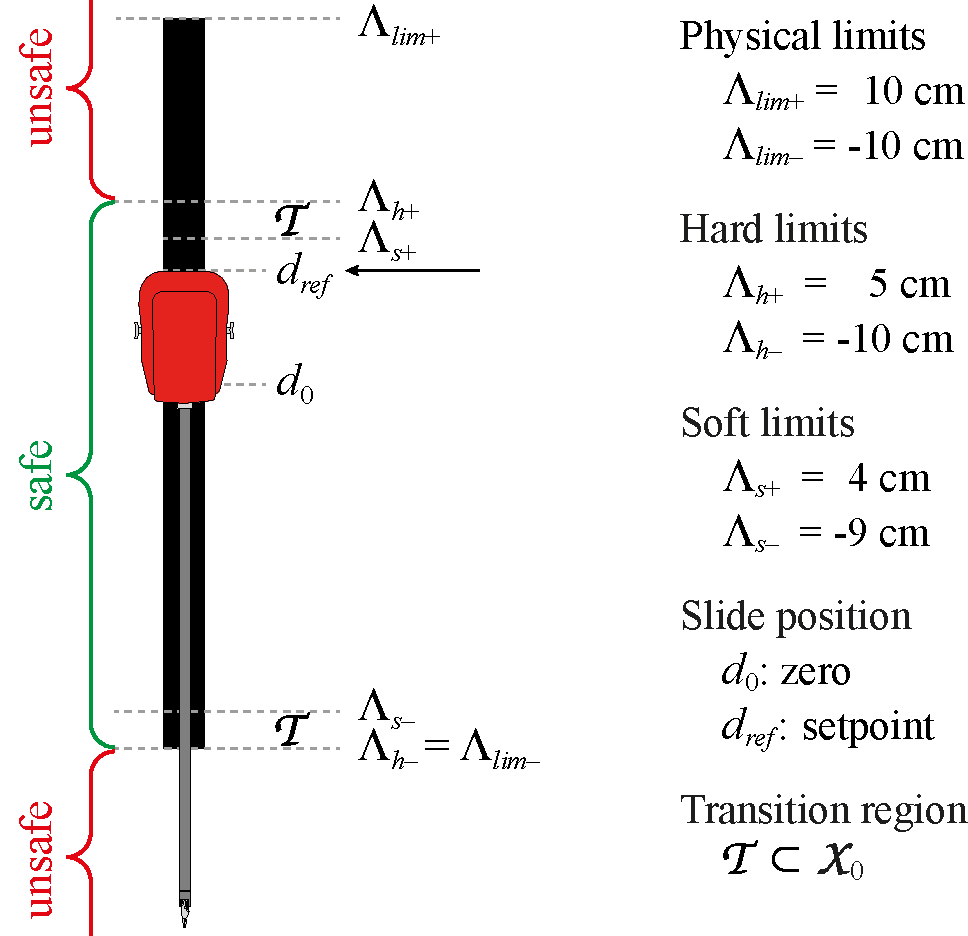
\includegraphics[width=0.42\textwidth]{slide_overview.pdf}\label{fig:safe:overview}}%
\caption{The slide position of the robotic instrument is visualized for the instrument house. As the remaining robot joints are not considered in this chapter, there is a one-to-one translation between instrument house position and instrument tip position. Slide house position in $d_0$ corresponds to tool tip position in zero in the $z$-dimension.}
\label{fig:slide}
\end{figure}
The boundaries for the slide position are summed up in \autoref{tab:intervals}.
\begin{table}[H]
	\begin{tabularx}{\textwidth}{X X X }
\rowcolor{HeaderBlue} 
$\mathcal{X}$ & $\mathcal{X}_u$  & $\mathcal{X}_0$ \\
$x \in \{[\Lambda_{\text{lim}-},\Lambda_{s-}],[\Lambda_{s+},\Lambda_{\text{lim}+}]\}$  & $x \in \{[\Lambda_{\text{lim}-},\Lambda_{h-}],[\Lambda_{h+},\Lambda_{\text{lim}+}]\} $ & $x \in \{[\Lambda_{h-},\Lambda_{s-}],[\Lambda_{s+},\Lambda_{h+}]\}$  \\
\end{tabularx}
\caption{Global state intervals for the position where: $\Lambda_\text{lim}$ is the physical slide limit ($\pm$0.1\,m), $\Lambda_s$ is a soft limit denoting a transition line and $\Lambda_h$ is a hard limit where a trajectory at all cost can not cross. The interval $x \in [\Lambda_{s-},\Lambda_{s+}] = \mathcal{Y}$ is safe thus $\tilde{u}(x)$ stated in \autoref{eq:utilde} can be used in this region.}
\label{tab:intervals}
\end{table}
As the control law stated in \autoref{eq:control_law} utilizes Lie derivatives, a system model is required before any controller design may be initiated.
%\hspace{1cm }\texttt{rostopic echo joint\_states/position[6]} \hspace{0.2cm} {\color{blue}{\# Be sure to have the ROS environment correctly configured according to \autoref{app:ros}}}
\section{Modelling of Slide Movement}\label{sec:model_slide}
To obtain a model of the slide movement, the step response will be measured.  This can be done by subscribing to the \texttt{joint\_state} topic in \gls{ros} (topics are ROS syntax for communication lines, see \autoref{app:ros} for an introduction to ROS). The experiment is described in further details in \autoref{app:meas}, and the result is plotted in \autoref{fig:stepresponseslide}. 
\begin{figure}[H]
\center
\includegraphics[scale=0.6]{step_slide.eps}
\caption{Step response from 0\,mm to 5\,mm. Plot details and measurements can be found in \autoref{app:cd} as \texttt{matlab\_scripts/slide\_step/plot\_slide\_pos.m}. The experiment is described in \autoref{app:meas}.}
\label{fig:stepresponseslide}
\end{figure}
The system can clearly be approximated with an underdamped second order model, however, for initial simplicity, merely a simple first order model of the slide movement is used. It shall, however, also be approximated as a second order system. This introduces a number of other challenges which is the reason for initial simplicity. These models will throughout this chapter be referred to as:
\begin{itemize}
\item One dimensional (1D) slide movement along the $z$-axis based on \underline{position} only, hence a first order system model.
\item One dimensional (1D) slide movement along the $z$-axis based on \underline{position and velocity}, hence a second order system model.
\end{itemize}
A first order approximation of the state space system will be modelled first. 
\subsection{1D Model based on Position}\label{subsec:model_1d}
The system can be approximated to a linear first order system with a dominating time constant \gls{taus}. The time constant is read from \autoref{fig:stepresponseslide}:
\begin{flalign*}
\tau_s = 110\, \text{ms}
\end{flalign*} 
A linear system can be outlined as:
\begin{flalign}
Y(s) &= \dfrac{1}{\tau_s s + 1}U(s) \nonumber\\
&=  \dfrac{1/\tau_s}{s + 1/\tau_s}\,U(s) = (s+1/\tau_s)^{-1}\,1/\tau_s\,U(s) \qquad\kk \overset{\overset{Y(s)=(C(sI-A)^{-1}B+D)U(s)}{\longrightarrow}}{\scriptsize \text{compare to obtain SS form}}  \nonumber\\ 
& \dot{x} = \underbrace{-\tau_s^{-1}\,x}_{Ax} + \underbrace{\tau_s^{-1}}_{B} u
\label{eq:1storder_1D_ss}
\end{flalign}
The system matrix $A$ and the input matrix $B$ can be read from the above equation:
\begin{flalign}
A = - \tau_s^{-1} =  \kk \wedge \kk B = \tau_s^{-1} \kk \wedge \kk C = 1 \kk \wedge \kk D = 0
\end{flalign}
Which completes the first order approximation.

\subsection{1D Model based on Position and Velocity}\label{subsec:model_2d}
The second order approximation is based on the form:
\begin{flalign}
\dfrac{Y(s)}{U(s)} = \dfrac{\omega_n^2}{s^2 + 2\zeta \omega_n s + \omega_n^2}
\label{eq:2order}
\end{flalign}
\begin{tabular}{rll} 
where  & & \\
$Y(s)$ & is the output in the Laplace domain  & [m] \\
$U(s)$ & is the input in the Laplace domain  & [m] \\
\gls{omegan} & is the natural frequency of the system & [rad/s] \\
\gls{zeta} & is the damping coefficient  & [$\cdot$] \\
$s$ & is the Laplace operator  & [rad/s] \\
\end{tabular}\\

The model can unambiguously be approximated from the rise time $t_r$, settling time $t_s$ (5\,\% settling time) and the overshoot $M_p$ \citep{bib:dynamicsystems}. They are measured (conservatively) from \autoref{fig:stepresponseslide} with the purpose to find $\omega_n$ and $\zeta$:
\begin{flalign*}
\omega_n &= \dfrac{1.8}{t_r} = \dfrac{1.8}{0.106\,\text{s}} = 17 \,\text{rad/s} \\
\zeta &= \dfrac{-1}{\omega_n \cdot t_s}\log (0.05) = \dfrac{-1}{17 \cdot 0.320}\log(0.05) = 0.55
\end{flalign*}
\Autoref{eq:2order} can be transformed into state space form: 
\begin{subequations}
\begin{flalign*}
Y(s)s^2 + 2\zeta \omega_n Y(s) s + \omega_n^2 Y(s) - \omega_n^2 U(s)  &= 0 \\
\ddot{y}(t) + 2\zeta \omega_n \dot{y}(t) + \omega_n^2 y(t) - \omega_n^2 u(t) &= 0 
\end{flalign*}
Choose $y(t) = x_1(t) =$ position, and let $\dot{x}_1(t) = x_2(t)$
\begin{flalign}
\begin{bmatrix}
\dot{x}_1(t)\\\dot{x}_2(t)
\end{bmatrix} &= 
\begin{bmatrix}
0 & 1\\
-\omega_n^2  & -2\zeta \omega_n  
\end{bmatrix}
\begin{bmatrix}
x_1(t) \\ x_2(t)
\end{bmatrix} + 
\begin{bmatrix}
0\\\omega_n^2
\end{bmatrix}u(t) \label{eq:2ndorder_1D_ss}\\
y(t) &= 
\begin{bmatrix}
1 & 0
\end{bmatrix}
\begin{bmatrix}
x_1(t) \\ x_2(t)
\end{bmatrix}
\end{flalign}
\end{subequations}
\begin{tabular}{rll} 
where  & & \\
$x_1(t)$ & is the position& [m] \\
$x_2(t) = \dot{x}_1(t)$ &is the velocity  & [m/s] \\
$y(t)$ & is the output (slide position)  & [m] \\
$u(t)$ & is the control input  & [$\cdot$]\\
\end{tabular}\\

Thus the linear system matrices can be outlined as:
\begin{flalign}
A = \begin{bmatrix}
0 & 1\\
 -\omega_n^2   & -2\zeta \omega_n 
\end{bmatrix} \kk \wedge \kk B = \begin{bmatrix}
0 \\ \omega_n^2
\end{bmatrix} \kk \wedge \kk C = \begin{bmatrix}
1 & 0
\end{bmatrix} \kk \wedge \kk D = 0 \label{eq:system:2}
\end{flalign}
Which completes the second order model.

\section{Construction of CBF}\label{sec:construct_cbf}
To illustrate the usefulness of \glspl{cbf}, a palpable example hereof will be created with direct application to the Da Vinci robot. This example does not directly constitute application to a patient but favour the theory in a neat and comprehensible sense and secure a way to visually and physically verify the method.
%
%Consider the state intervals defined in \autoref{tab:intervals}.
%
%
\subsection{Construction of CBF based on First Order Model}\label{subsec:cbf-1order}
In this subsection, the state vector $x \in \mathbb{R}$ consists of the position only. Thus, a parabola is now introduced as \gls{cbf} as it allows an easy way to define $\mathcal{X}_u$ and $\mathcal{X}_0$ from \autoref{tab:intervals}. %A coordinate shift is performed such that the slide movement occurs along the $x$-axis instead of the $z$-axis. 
\begin{flalign}
B(x) &= ax^2+bx+c \label{eq:cbf1} 
\end{flalign}
The parameters $a$, $b$ and $c$ can be easily chosen to fulfil the requirements in \autoref{cer1} and \ref{cer2} for a barrier function, thereby fulfilling the parallel requirements for the \gls{cbf} in \autoref{req1} and \ref{req3}. From \autoref{req2} it is required that either $L_gB(x) \neq 0 \,\,\,\forall x\in \mathcal{X}$, or that $L_fB(x)<0$ when $L_gB(x) = 0$, as the input in that case will be insignificant. Analysing $L_gB(x) = 0$
\begin{flalign*}
	L_gB(x) \Bigm|_{g(x)=B} = ( 2ax + b ) \cdot \tau^{-1} = 0 \kk \Rightarrow \kk x = \dfrac{-b}{2a}\label{eq:LgB_1D}
\end{flalign*}
it is seen that this is only the case in $x = \tfrac{-b}{2a}$ which is indeed the critical point for a one dimensional parabola. As is the case for Lyapunov functions (see  \autoref{eq:lyap_vdot_minus_criticalpoint}) in the critical point the requirement on the derivative is relaxed to  $L_fB(x) \leq 0$.   
\begin{flalign}
L_fB(x) = \dfrac{d}{dx}B(x)f(x)\Bigm|_{f(x)=Ax}  &= (2ax+b)(-\tau^{-1}x) = -2\tau^{-1}ax^2-\tau^{-1}bx \nonumber\\
L_fB(x)\Bigm|_{x= \frac{-b}{2a}} &= -2\tau^{-1}a\left(\frac{-b}{2a}\right)^2-\tau^{-1}b\left(\frac{-b}{2a}\right) = 0\nonumber
%0 \kk \Leftrightarrow \kk  -2\tau^{-1}ax^2-\tau^{-1}bx = 0 \nonumber
% \\  &-2ax^2-bx = 0 \mm \Rightarrow \mm x = 
%\begin{cases}
%  \frac{-b}{2a} \\
%   0   
%\end{cases}
\label{eq:interval1}
\end{flalign}
Hence the \gls{cbf} is valid for all choices of $a,b$. The scalar $c$ must be less than zero to comply with \autoref{req3}.
At this point in time, three equations with three unknowns can be outlined to fulfil the initial demand in \autoref{fig:safe:overview}.
\begin{flalign*}
 \left.
 \begin{aligned}
a\,\Lambda_{h+}^2 + b\,\Lambda_{h+} + c = 0 \\
a\,\Lambda_{h-}^2 + b\,\Lambda_{h-} + c = 0 \\
a\left( \frac{\Lambda_{h-}+\Lambda_{h+}}{2}\right)^2 + b\left(\frac{\Lambda_{h-}+\Lambda_{h+}}{2}\right) + c = \underbrace{-0.025}_\text{any constant $<0$} 
\end{aligned}
\mm \right\}
 \qquad \begin{matrix}
 a &= \,\,\,\,\,\,\,\,1.7778 \\ b &= \,\,\,\,\,\,\,\,0.0889 \\ c &= -0.0089
 \end{matrix}
\end{flalign*}
%The interval where $B(x)$ is invalid can thereby be found from \autoref{eq:interval}:
%\begin{flalign*}
%B(x) \hspace{0.15cm} \text{invalid:} \mm  x \in [-0.0250,0] \kk \text{if} \mm L_gB(x) = 0
%\end{flalign*}
%However, this is indifferent as $\{\mathcal{X} \,\bigcap\, [\Lambda_{s-},\Lambda_{s+}]  \} = \emptyset $. Thus the barrier function is a valid \gls{cbf}. It is plotted in \autoref{fig:barrierfunction}
The \gls{cbf} is plotted in \autoref{fig:barrierfunction} from which it is seen that the demands from \autoref{tab:intervals} are fulfilled.
\begin{figure}[H]
\center
	\includegraphics[scale=0.63]{parabel_1.eps}
	\caption{Barrier function shown along with the $\mathcal{X}_u$ and $\mathcal{X}_u^c$. Plot details and MATLAB script can be found in \autoref{app:cd} as \texttt{matlab\_scripts/plot\_parabola/plot\_parabola.m}}
	\label{fig:barrierfunction}
\end{figure}
%\underline{Note:} The above analysis ensures safety regardless of $L_gB(x) = 0$ as it merely takes place at the critical point, i.e.:
%\begin{flalign*}
% L_gB(x) = (2ax+b)B = 2ax\tau^{-1} + b\tau^{-1} = 0 \kk \Leftrightarrow \kk 2ax = -b \kk \Leftrightarrow \kk x = \dfrac{-b}{2a}
% \end{flalign*} 
% This is again the parabola extremity as it was found in \autoref{eq:interval1} and in fact an allowed exception for condition \autoref{req2} as the system is in its equilibrium.

\subsection{Construction of CBF Based on Second Order model}\label{subsec:cbf-2order}
Consider now for the second order system the same candidate \gls{cbf} as given in \autoref{eq:cbf1}. Note that $B(x)$ is a function of position only, such that the CBF is:
\begin{flalign*}
B(x_1) = a\,x_1^2+ b\,x_1 + c
\end{flalign*}
For this system model the Lie derivative $L_gB(x)=0\,\,\forall x$:
\begin{flalign*}
L_gB(x) = \dfrac{d B(x)}{d x}g(x) \Bigm|_{g(x)=B} =  
\begin{bmatrix}
\dfrac{\partial B(x)}{\partial x_1} & \dfrac{\partial B(x)}{\partial x_2} 
\end{bmatrix}\begin{bmatrix}
0 \\ \omega_n^2
\end{bmatrix} = 0 \label{eq:LgB_secondorder_invalid}
\end{flalign*}
This puts forth the requirement that $L_fB(x)<0\,\,\, \forall \, x$. Accordingly:
\begin{flalign*}
L_fB(x) = \dfrac{d B(x)}{d x}f(x) \Bigm|_{f(x)=Ax} &= 
\begin{bmatrix}
\dfrac{\partial B(x)}{\partial x_1} & \dfrac{\partial B(x)}{\partial x_2} 
\end{bmatrix}
\begin{bmatrix}
0 & 1 \\
-\omega_n^2 & -2\zeta\omega_n
\end{bmatrix} \begin{bmatrix}
x_1 \\ x_2
\end{bmatrix} \nonumber \\
&= (2ax_1+b) x_2 - 0\cdot(\omega_n^2 x_1 + 2\zeta \omega_n x_2) \nonumber \\
&= 2ax_1x_2 + bx_2
\label{eq:2d_x1}
\end{flalign*}
Note that the velocity appears in both terms. As the velocity can be both decreasing and increasing for all positions, this demand is impossible to fulfil with this candidate \gls{cbf}  and it is therefore invalid. A solution may be to include the velocity in the barrier function. 

Safety constraints on velocity are not of any significant importance as such, but they are necessary for $L_gB(x)$ to obtain values different from zero as opposed to the Lie derivative of the invalid \gls{cbf} $B(x_1)$.
Consider instead the elliptic paraboloid as \gls{cbf}:
\begin{flalign}
B(x_1,x_2) =  \left( \dfrac{(x_1-x_{10})^2}{a_2^2} + \dfrac{(x_2-x_{20})^2}{b_2^2} \right) c_1 + c_2
\label{eq:cbf2}
\end{flalign}
\begin{tabular}{rp{13.7cm}l} 
where  & & \\
$x_1$& is the position  & [m] \\
$x_2$& is the velocity & [m/s] \\
$x_{10}$& is the extremity point for $x_1$ and thereby equilibrium point for an upward paraboloid & [m] \\
$x_{20}$& is the extremity point for $x_2$ and thereby equilibrium point for an upward paraboloid & [m/s] \\
$a_2$& is a constant that dictates the level of curvature in the $x_1-B(\textbf{x})$ plane & [$\cdot$] \\
$b_2$& is a constant that dictates the level of curvature in the $x_2-B(\textbf{x})$ plane & [$\cdot$] \\
$c_1$ & is a constant that dictates if the paraboloid points upward ($c_1>0$) or downward ($c_1 < 0$)& [$\cdot$]  \\
$c_2$ & is a constant that dictates the offset in $B(\textbf{x})$ axis & [$\cdot$] \\
\end{tabular}\\

The elliptic paraboloid allows constraints on both position and velocity.  To ensure that the position demands from \autoref{tab:intervals} are still fulfilled and are so for all possible velocities (constrained by the slide movement's physical limits), the below values are chosen:
\begin{flalign*}
x_{10} &= \dfrac{\Lambda_{h-}+\Lambda_{h+}}{2} = -0.025 \\
x_{20} &= 0\\
\mathcal{M}_{B(x)=0} &= 4
%\Lambda_{x2-} &= -4 \kk \text{denotion of the lowest value where $B(0,x_2)=0$} \\
%\Lambda_{x2+} &= 4 \kk \text{denotion of the highest value where $B(0,x_2)=0$} 
\end{flalign*}
\begin{figure}[htbp]
	\centering
	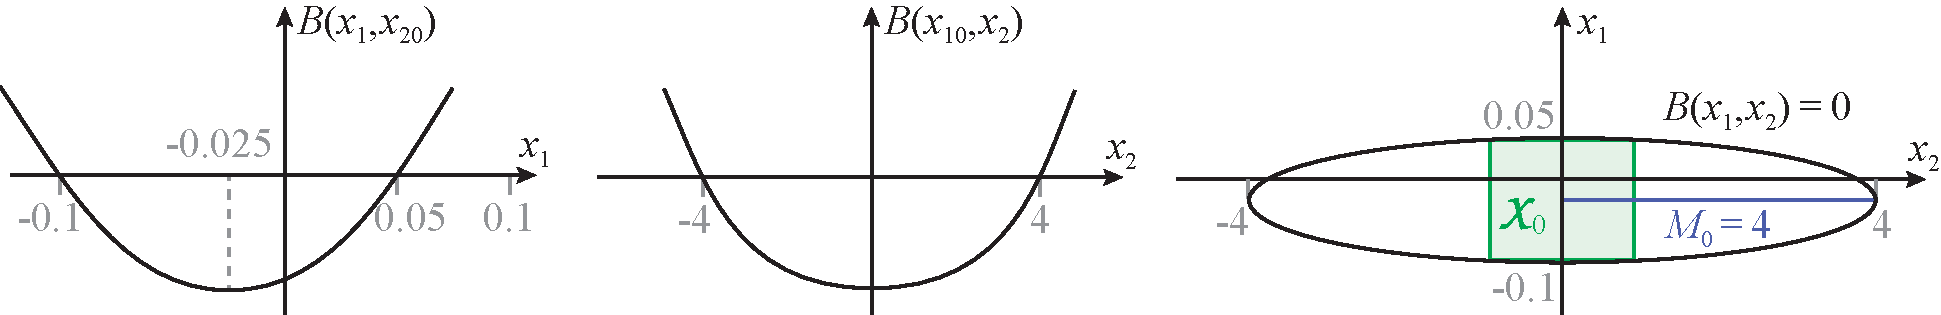
\includegraphics[width=\textwidth]{cbf_2ndorder.pdf}
	\caption{Choice of critical point coordinate $x_{10}$  as the middle of the safe position interval. The semimajor axis of the \gls{cbf}'s zero level set is chosen much larger than the physical limits  of the slide velocity.}
	\label{fig:cbf_2ndorder}
\end{figure}

where $\mathcal{M}_{B(x)=0}$ denotes the semimajor axis of the zero level set of the \gls{cbf}.
Note that $x_{20}$ ensures velocity equilibrium in 0\,m/s and note that the velocity outermost points are determined far bigger than the robot's physical limits to ensure that all position values on the interval  $[-0.1\,\,\,\,0.05]$ are considered safe (almost) independently of the velocity. % $\mathcal{X}_0 \notin \mathcal{X}_u $. 
This is sketched in \autoref{fig:cbf_2ndorder} along with the chosen values.

Having chosen the coordinates $x_10$ and $x_{20}$ for the critical point, an arbitrary negative value is chosen for $B(x_{10},x_{20})$, and using the four known coordinates from the zero level set $(\Lambda_{h+},0)$, $(\Lambda_{h-},0)$, $(x_{10},-4)$ and $(x_{10},4)$, five equations with four unknowns can be outlined with the below numerical values.
\begin{flalign*}
 \left.
\begin{aligned}
\left( \dfrac{\left(\frac{\Lambda_{h-}+\Lambda_{h+}}{2}-x_{10}\right)^2}{a_2^2} + \frac{(0-x_{20})^2}{b_2^2} \right)c_1 + c_2 =  \underbrace{-1.000}_\text{any constant $<0$} \\
\left(\dfrac{(\Lambda_{h+}-x_{10})^2}{a_2^2} +\frac{(0-x_{20})^2}{b_2^2}\right) c_1 + c_2 = 0 \\
 \left(\dfrac{(\Lambda_{h-}-x_{10})^2}{a_2^2}+\frac{(0-x_{20})^2}{b_2^2}\right) c_1 + c_2 = 0 \\
 \left(\dfrac{\left(\frac{\Lambda_{h-}+\Lambda_{h+}}{2}-x_{10}\right)^2}{a_2^2} +\dfrac{(4-x_{20})^2}{b_2^2} \right)c_1 + c_2 = 0 \\
\left(\dfrac{\left(\frac{\Lambda_{h-}+\Lambda_{h+}}{2}-x_{10}\right)^2}{a_2^2} + \dfrac{(-4-x_{20})^2}{b_2^2}\right) c_1 + c_2 = 0 
% \dfrac{\left(0-x_{20}\right)^2}{b_2^2} c_1 + c_2 =  \underbrace{-1.000}_\text{any constant $<0$}  
\end{aligned}
\mm \right\}
 \qquad 
\begin{matrix*}[r]
x_{10} &=& -0.025 \\ 
x_{20} &=&  0.000 \\
B(x_{10},x_{20}) &=&   -1.000\\
&&\\
a_2 &=& 0.075 \\ 
b_2 &=& 4.000 \\
c_1 &=& 1.000 \\ 
c_2 &=& -1.000
\end{matrix*}
\end{flalign*}
The Lie derivatives can now be calculated as:
\begin{flalign}
L_gB(x_1,x_2) &= \dfrac{d B(x_1,x_2)}{d x} \cdot g(x) \Big|_{g(x)=\textbf{B}} = \begin{bmatrix}
\dfrac{\partial B(x_1,x_2)}{\partial x_1} & \dfrac{\partial B(x_1,x_2)}{\partial x_1}
\end{bmatrix}  \begin{bmatrix}
0 \\ \omega_n^2
\end{bmatrix} \nonumber \\
 &= \begin{bmatrix}
 \dfrac{c_1(2x_1 - 2x_{10})}{a_2^2} &  \dfrac{c_1(2x_2 - 2x_{20})}{b_2^2}
\end{bmatrix}  \begin{bmatrix}
0 \\ \omega_n^2
\end{bmatrix} = 
\dfrac{c_1\omega_n^2(2x_2-2x_{20})}{b_2^2} \Bigm|_{x_{20}=0} \nonumber\\
&= \dfrac{2c_1\omega_n^2}{b_2^2} x_2
\label{eq:LgB_2}
\end{flalign}
It is seen that $L_gB(x_1,x_2) \neq 0 \mm \forall \,\,\, x_2 \neq 0$, hence $L_fB(x_1,x_2)$ is for that reason analysed and evaluated at $x_2=0$:
\begin{flalign}
L_fB(x_1,x_2) &= 
\dfrac{\partial B(x_1,x_2)}{\partial x} f(x)\Big|_{f(x) = \textbf{Ax}} = \begin{bmatrix}
\dfrac{\partial B(x_1,x_2)}{\partial x_1} & \dfrac{\partial B(x_1,x_2)}{\partial x_1}
\end{bmatrix} \begin{bmatrix}
0 & 1 \\
-\omega_n^2 & -2 \zeta \omega_n
\end{bmatrix} \begin{bmatrix}
x_1 \\ x_2
\end{bmatrix} \nonumber\\
&= \begin{bmatrix}
 \dfrac{c_1(2x_1 - 2x_{10})}{a^2} &  \dfrac{c_1(2x_2 - 2x_{20})}{b^2}
\end{bmatrix} \begin{bmatrix}
x_2 \\ -\omega_n^2 x_1 - 2\zeta \omega_n x_2
\end{bmatrix} \nonumber\\
&= \dfrac{c_1x_2(2x_1-2x_{10})}{a_2^2} - \dfrac{c_1(2x_2-2x_{20})(\omega_n^2 x_1+2\zeta \omega_n x_2 )}{b_2^2} \Big|_{x_{20} = 0} \nonumber\\
&= \left( \dfrac{2c_1(x_1+x_{10})}{a_2^2} - \dfrac{2c_1(\omega_n^2 x_1 +2\zeta \omega_n x_2)}{b_2^2} \right) x_2 \Big|_{x_{2} = 0} = 0
\label{eq:LfB_2}
\end{flalign}
It is noted that $L_fB(x_1,x_2) = 0$ for $x_2 = 0$ which implies stability but not asymptotic stability. That is in general not good for physical systems and does not fulfil \autoref{req2}. It does, however, fulfil \autoref{req2_weak} thus proving $B(x_1,x_2)$ to be a weak \gls{cbf}. %However, an engineering reflection and decision is taken at this point.
Note that when the velocity is zero, the slide movement is steady, although only marginally stable. %At this point $k_0(x)=0$, which indeed will force the slide movement to its origin as the control signal is the reference to a position controller. 
As an engineering reflection it is considered that when the state leaves the marginally stable equilibrium, $x_2 \neq 0$, and the safety controller $k_0(x)$ will ensure that the state will increase its distance to the unsafe set and go towards its stable equilibrium in $(x_{10},x_{20})=(-0.025,0)$. 
%It implies hereafter $x_2 \neq 0$ again which is sufficient for the safety controller. %That is in this case a good thing as the slide will move back to the safe region and away from $\Lambda_{h-}$ and $\Lambda_{h+}$. Lastly, the velocity will never be truly zero due to the finite resolution, i.e. a finite sampling rate. For these reasons, the \gls{cbf} from \autoref{eq:cbf2} is accepted, well aware that the \gls{cbf} is insufficient,. It is, however, important to keep in mind that this is a dangerous decision. {\color{green}{RAFAL: Er det overhovedet OK at sige s\aa dan?}}


\begin{figure}[H]
\hspace*{-2mm}
	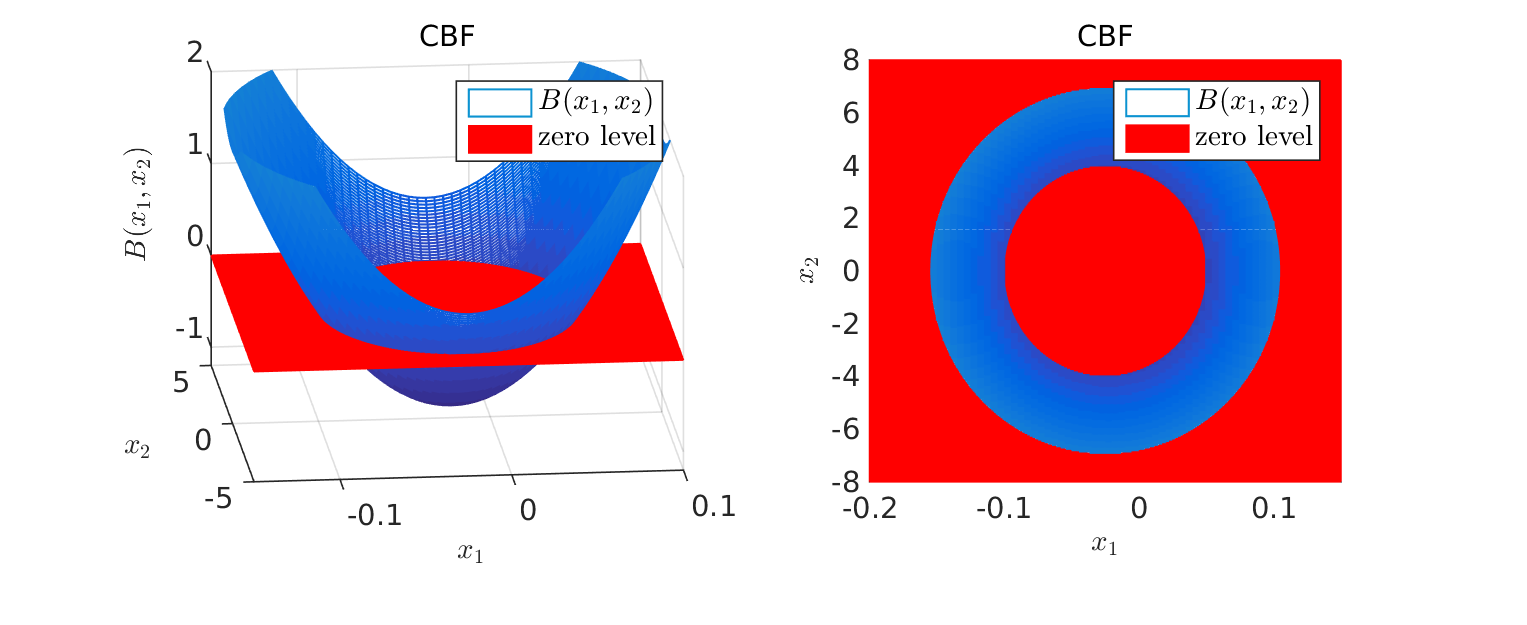
\includegraphics[width=1.02\textwidth]{cbf_2d.eps}
	\vspace*{-11mm}
	\caption{CBF for the second order system model. Plot details and MATLAB script can be found in \autoref{app:cd} as \texttt{matlab\_scripts/plot\_cbf\_2d/plot\_cbf\_2d.m}}
	\label{fig:barrierfunction_2d}
\end{figure}
The elliptic paraboloid with its proper boundaries is plotted in \autoref{fig:barrierfunction_2d}, from which it is seen how $B(x_1,x_2)<0$ only within the specified regions, i.e. $x_2 \in [-\mathcal{M}_{B(x)=0},\mathcal{M}_{B(x)=0}]$ and $x_1 \in [\Lambda_{h-},\Lambda_{h+}]$. %, and thus everything else is unsafe, i.e. $B(x) > 0$. 
It is also seen that for small velocities (physically $x_{2,\text{max}}\approx 1$\,m/s) the \gls{cbf} is approximately vertical in the boundaries of $x_1$ %when the big numerical difference in the axes is taken into account.
leaving $\mathcal{X}_0$ almost independent of the velocity, as prescribed in \autoref{fig:cbf_2ndorder}.

\begin{figure}[H]
	\centering
	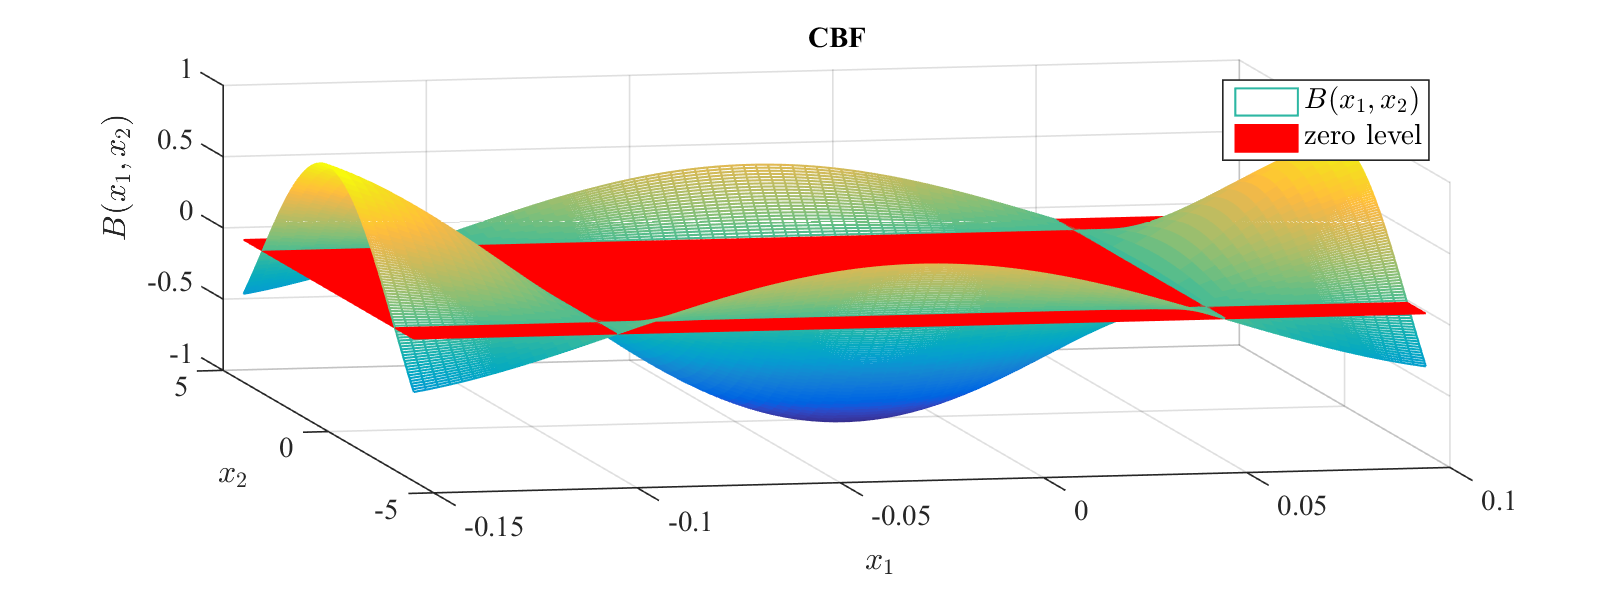
\includegraphics[width=.95\textwidth]{cbf_example_sinus.eps}
	\caption{CBF. Example to demonstrate how other CBFs suffer when $x_2 = 0$.}
	\vspace{-7mm}
	\label{fig:barrierfunction_example_sinus}
\end{figure}
\vspace{5mm}

\textbf{\underline{\textit{Remark:}}} The issue caused by $x_2=0$ is not only the case for this specific \gls{cbf} but for many \gls{cbf}s. Take for example another CBF that could fulfil the position requirements from \autoref{tab:intervals}:
\begin{flalign*}
B(x_1,x_2) = \cos (c_3 x_1 + c_4) \cdot \cos (c_5 x_2 + c_6)
\end{flalign*}
It turns out that the coefficients $c_3 = 21.00, c_4 = 119.91, c_5 = 0.50, c_6 = 3.15$ induce a CBF with the same properties as the one depicted in \autoref{fig:barrierfunction_2d}. The \gls{cbf} is outlined graphically in \autoref{fig:barrierfunction_example_sinus}.

Thus $L_gB(x_1,x_2)$ can be found as:
\begin{flalign*}
L_gB(x_1,x_2) = -c_5 \omega_n^2 \cos (c_3 x_1+c_4)\sin(c_5 x_2+c_6)
\end{flalign*}
Now note that $L_gB(x_1,x_2) = 0$ when $c_6+c_5x_2 = i\pi$, $i\in\mathbb{Z}$, which is true for e.g. $x_2 \approx 0$. This implies the requirement that $L_fB(x_1,x_2) < 0$ whenever $x_2 \approx 0$. % As $L_gB(x_1,x_2) \neq 0 \,\, \forall \,\, x_2 \approx 0$, requirements for $L_fB(x_1,x_2)$ is necessary. 
However, taking a look at $L_fB(x_1,x_2)$:
\begin{flalign*}
L_fB(x_1,x_2) = 
c_5\cos (c_3 x_1+c_4 ) \sin(c_5 x_2+c_6)( \omega_n^2 x_1 + 2  \zeta \omega_n x_2) - c3 x_2 \cos( c_5 x_2+c_6) \sin( c_3 x_1+c_4)
\end{flalign*}
quickly poses the fact that $L_fB(x_1,x_2 )$ is not necessarily negative for $x_2 \approx 0$ due to the sign alternation caused by the term $\sin(c_3 x_1+c_4)$ in the boundaries.

\section{Control Design}
\vspace*{-1mm}
This section constitutes the design of the two controllers. The controller based on the first order approximation is straight forward whereas the controller based on the second order approximation requires an observer because the velocity cannot be measured.
\subsection{Control Design based on First Order
	\vspace*{-1mm} Model}\label{sec:K_Nbar_1D_1storder}
To be able to find $k_0(x)$ from \autoref{eq:control_for_safety}, the constant $\epsilon$ used in \autoref{eq:smoothness} must be found. It can be determined from the \gls{cbf} from \autoref{eq:cbf1} such that it complies with the requirements from \autoref{tab:intervals}:
\begin{flalign}
\epsilon = |B(\Lambda_{s+})| = |B(\Lambda_{s-})| = 0.00249
\label{eq:epsilon}
\end{flalign}
Utilizing $\sigma(x)$ as described in \autoref{eq:smoothness} secures a neat way to incorporate the transition between $\Lambda_s$ and $\Lambda_h$ because the safety controller $k_0(x)$ gradually takes over when the trajectory exceeds $\Lambda_s$. \Autoref{fig:epsilon_plot} illustrates how $\epsilon$ and $B(x)$ are connected.
\begin{figure}[H]
	\center
		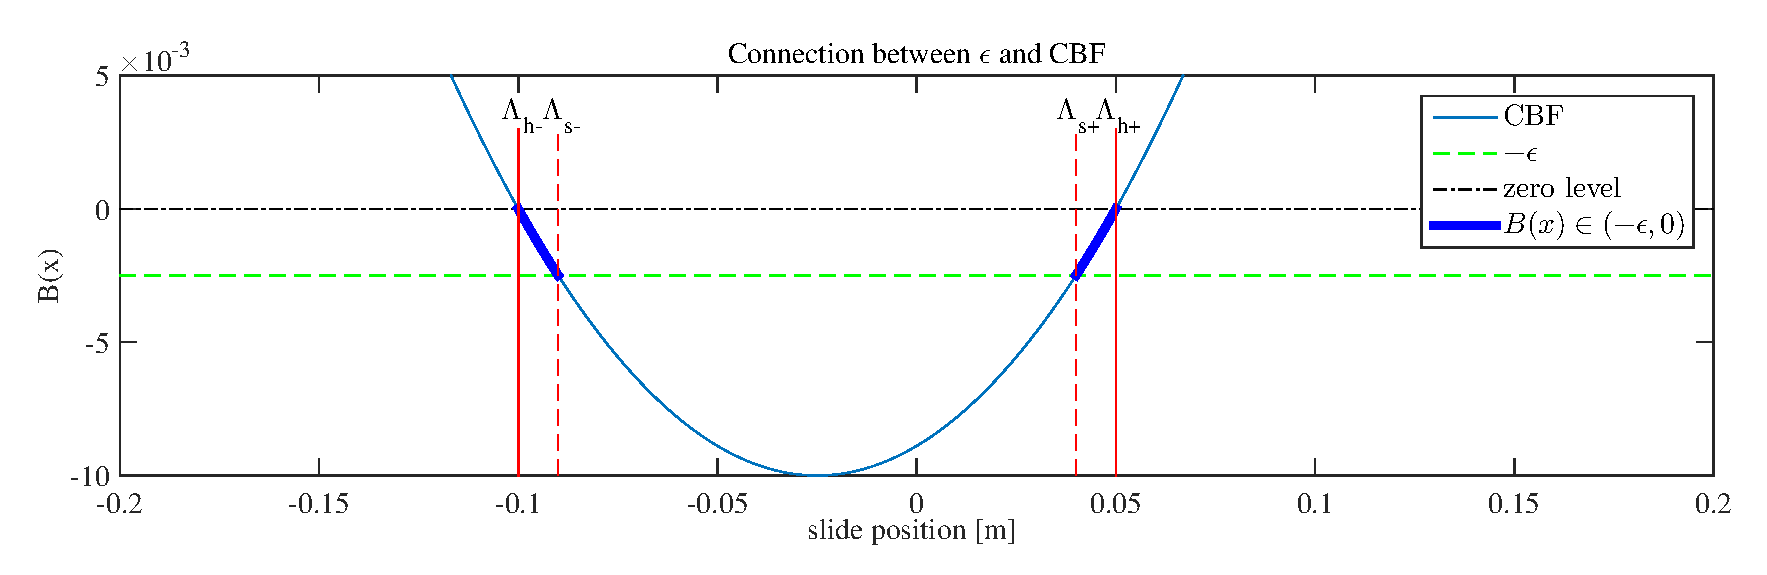
\includegraphics[scale=0.55]{epsilon_plot.eps}
	\caption{Connection between $\epsilon$ and CBF. MATLAB script and plot details can be found in \autoref{app:cd} as \texttt{matlab\_scripts/plot\_epsilon/plot\_epsilon\_slide\_1d.m}}
	\label{fig:epsilon_plot}
\end{figure}

The system is approximated as a linear system on the form $\dot{x}=Ax+Bu$, thus pole placement can be used. No constraints to the constant feedback matrix $K$ will be outlined except stability. It will therefore be determined from the pole placement method where a closed loop pole that is ten times faster than the open loop pole will be placed. Ackermann's formula can be used \citep{bib:acker}:
\begin{enumerate}
\itemsep-3mm
\item Identify the desired closed loop polynomial as $A_{cl}(s) = s^n + a_{c(n-1)}s^{n-1}  +  \cdots + a_ {c1}s + a_{c0}$: 
\vspace*{-1mm}
\begin{flalign*}
A_{cl}(s) = s + 10\,\tau^{-1}
\end{flalign*}
\item Identify the open loop polynomial as $A_{ol}(s) = s^n + a_{n-1}s^{n-1} +  \cdots + a_1s + a_0$: 
\vspace*{-1mm}
\begin{flalign*}
A_{ol}(s) = \lambda + \tau^{-1}
\end{flalign*}
\item Compute the feedback matrix in controllable canonical form:
\vspace*{-1mm}
\begin{flalign*}
 \bar{K}^T = \begin{bmatrix}   
 \bar{k_1} \\
 \vdots \\
 \bar{k_n}
 \end{bmatrix} = \begin{bmatrix}
 a_{c0} - a_0 \\
 \vdots \\
 a_{c(n-1)} - a_{n-1}
 \end{bmatrix} \kk \Rightarrow  \kk \bar{K}^T = 10\,\tau^{-1} - \tau^{-1} = 9\,\tau^{-1}
\end{flalign*}
\vspace*{-1mm}
\item Compute the similarity transform $Q$ recursively as: 
\vspace*{-1mm}
\begin{flalign*}
Q = \begin{bmatrix}
q_1 & q_2 & \cdots & q_n
\end{bmatrix} \qquad
\Rightarrow \qquad
Q = \tau^{-1}
\end{flalign*}
\vspace*{-1mm}
\begin{tabular}{rl}
where&\\
$ q_n$&\hspace{-3mm}$ = \textbf{B}$ \\
$ q_{j-1}$&\hspace{-3mm}$ = A\,q_j + a_{j-1}B$\\
\end{tabular}\\\\

\item Compute the feedback matrix as:
\vspace*{-1mm}
\begin{flalign}
K = \bar{K}\,Q^{-1} = 9\,\tau^{-1}\dfrac{1}{\tau^{-1}} = 9
\label{eq:K_1}
\end{flalign}
\end{enumerate}
The constant feedback matrix $\bar{N}$, ensuring unity gain between reference and output, can be computed as \citep{bib:Nbar}:
\vspace*{-3mm}
\begin{flalign}
\bar{N} = - \left( C\,A_{cl}^{-1}\,B \right)^{-1} =  - \left( C\,(A-B\,K)^{-1}\,B \right)^{-1} = 10
\label{eq:barm_1}
\end{flalign}
%\subsubsection*{Merged Control Law}
With the Lie derivatives computed as:
\begin{flalign}
L_fB(x) = -2\tau^{-1}ax^2-\tau^{-1}bx \kk \wedge \kk L_gB(x) = 2ax\tau^{-1} + b\tau^{-1}
\label{eq:lies_1}
\end{flalign}


\begin{recap}[Control Law for First Order Approximation]\label{recap:1d_static_1storder}

	The complete control law can be determined from \autoref{eq:control_law}:
\begin{flalign*}
u(x) = \sigma(x)k_0(x)+(1-\sigma(x))(\bar{N} \cdot x_\text{ref}-Kx) 
\end{flalign*}
\vspace{-0.8cm}
\begin{tabular}{rp{13.7cm}} 
where  & \\
$\sigma(x)$ & is computed from \autoref{eq:smoothness} with the $\epsilon$ found in \autoref{eq:epsilon} and the \gls{cbf} found in \autoref{eq:cbf1}  \\
$k_0(x)$ & is computed from \autoref{eq:control_law_safety} with the Lie derivatives stated in \autoref{eq:lies_1} \\
$\bar{N}$ & is found in \autoref{eq:barm_1}  \\
$K$ & is found in \autoref{eq:K_1} \\
\end{tabular}\\
\end{recap}
%\vspace{-0.2cm}
This completes the control design based on a first order system approximation. 



\subsection{Control Design Based on a Second Order Model}\label{sec:K_Nbar_1D_2ndorder}
A necessary condition for a controller is that the system is controllable:
\begin{flalign*}
 \mathcal{C} = \begin{bmatrix}
 B & A\,B
 \end{bmatrix} =  \begin{bmatrix}
 0 & \omega_n^2 \\
 \omega_n^2 & -2 \zeta \omega_n^3
 \end{bmatrix} \kk \text{thus} \mm \text{rank} ( \mathcal{C} ) = 2 = n \kk \Rightarrow \mm \text{controllable}
\end{flalign*} 
To design the smoothing in the transition space $\mathcal{T}$ for the second order approximation, the $\epsilon$ found in \autoref{eq:epsilon} is used again such that the \gls{cbf} from \autoref{eq:cbf1} is reused here. To allow the instrument some physical distance to brake and turn around (caused by the inertia), $\sigma(x)$ is multiplied by a scalar $c$ such that it reaches 1 before it is too late for the instrument to turn around. $\sigma(x)$ is however still limited to its maximum value at 1.
\begin{flalign}
\sigma(x) = 
\begin{cases}
0 & \text{if} \mm B(x) \leq -\epsilon \\
c\, \left( -2  \left( \dfrac{B(x}{\epsilon} \right)^3 - 3\left( \dfrac{B(x_1)}{\epsilon} \right)^2 +1 \right) \kk &\text{if} \mm B(x_1) \in (-\epsilon,0) \\
1  &\text{if} \mm B(x) \geq 0
\end{cases}
\end{flalign} 
At this point, two cases will be considered:
\begin{itemize}
\item \textbf{1.} Construction of $K$ and $\bar{N}$ in a similar way as in \autoref{sec:K_Nbar_1D_1storder}. This is possible in an ideal simulation because the velocity can be extrapolated by means of the forward euler approach (ideal design).
\item \textbf{2.} Development of an observer to estimate the velocity based on the model and position measurements. This is necessary on a real system.
\end{itemize}
\subsubsection{Design with the intention to simulate with Forward Euler}
The design of $K$ and $\bar{N}$ will follow the exact same procedure as described for the first order model except now $K \in \mathbb{R}^{1 \times 2}$. $\bar{N}$ remains as a scalar. The entire design procedure is therefore not carried through again.  

However, it is of interest to slow down the system dynamics slightly compared to the controller based on a first order system. This is to enter the unsafe region with a lower velocity and thereby allow the safety controller some transition space to navigate the trajectory back to its safe area. The eigenvalues of the second order system is found to:
\begin{flalign*}
\lambda_\text{2nd order system} = \begin{cases}
-10.295 -14.765\,j \\
-10.295 +14.765\, j
\end{cases}
\end{flalign*}
The feedback vector can be found with the MATLAB command \texttt{acker} based on pole placement slightly faster than the system itself.
\begin{flalign}
K = \texttt{acker(A,B,C,D,[-40 -50])} = \begin{bmatrix}
5.173  &  0.214
\end{bmatrix}
\label{eq:K_2}
\end{flalign}
The DC gain can now be corrected with:
\begin{flalign}
\bar{N} = - \left( C\,A_{cl}^{-1}\,B \right)^{-1} =  - \left( C\,(A-B\,K)^{-1}\,B \right)^{-1} = 6.173
\label{eq:Nbar_2}
\end{flalign}
These matrices are used in the MATLAB simulation.
\subsubsection{Observer Design}
A necessary condition for an observer is that the system is observable:
\begin{flalign*}
 \mathcal{O}= \begin{bmatrix}
 C \\ C A
 \end{bmatrix} =  \begin{bmatrix}
 1 & 0 \\
 0 & 1
 \end{bmatrix} \kk \text{thus} \mm \text{rank} ( \mathcal{O}) = 2 = n \kk \Rightarrow \mm \text{observable}
\end{flalign*} 
An observer (discrete version) with proper gain corrections can be designed as \citep{bib:Nbar}:
\begin{flalign}
\hat{x}(k+1) = \Gamma \hat{x}(k) + \Phi K_d \hat{x}(k) + L_d ( \underbrace{C\hat{x}(k)-y(k)}_\text{error} ) + M x_\text{ref}
\label{eq:observer}
\end{flalign}
\vspace{-0.6cm}
\begin{longtable}{p{.8\textwidth} p{.1\textwidth} p{.1\textwidth}} 
where  & & \\
$k$ is the current sample \\
\gls{Gamma} is the discretized system matrix \\
\gls{Phi} is the discretized input matrix \\
\gls{Kd} is control gain calculated from the discretized matrices \\
\gls{Ld} is observer gain calculated from the discretized matrices \\
\gls{M} is gain correction to ensure unity gain for the observer \\
\gls{N} is gain correction to ensure unity gain for the system  
\end{longtable}
\vspace*{-0.2cm}
The associated continuous system is:
\begin{flalign*}
\dot{x} &= A x + B(N x_\text{ref} - Kx) \\
y &= Cx
\end{flalign*}
The equations are implemented in simulink as shown in \autoref{fig:simulink_observer}.
\begin{figure}[H]
	\center
		\includegraphics[scale=0.6]{observer_2_order.pdf}
	\caption{Simulink implementation of the discrete observer.}
	\label{fig:simulink_observer}
\end{figure}
The augmented (discrete) system in $\mathbb{R}^{4 \times 4}$ will be outlined as:
\begin{flalign*}
\begin{bmatrix}
x(k+1) \\
\hat{x}(k+1)
\end{bmatrix} &= \underbrace{\begin{bmatrix}
\Gamma & \Phi K_d \\
L_d C & \Gamma + \Phi K_d + L_d C 
\end{bmatrix} }_{\Gamma_{cl}}\begin{bmatrix}
x(k) \\ \hat{x}(k)
\end{bmatrix} + \underbrace{\begin{bmatrix}
\Phi N \\ M
\end{bmatrix}}_{\Phi_{cl}} x_\text{ref} \\
y(k) &= \underbrace{\begin{bmatrix}
C & 0 & 0
\end{bmatrix}}_{C_{cl}}\begin{bmatrix}
x(k) \\ \hat{x}(k)
\end{bmatrix}
\end{flalign*}
The discrete matrices $\Gamma$ and $\Phi$ can be found as \citep{bib:discrete_sampling}:
\begin{flalign}
\Gamma &= \text{expm} (A\, T_s) = \begin{bmatrix}
0.986 & 0.009 \\
-2.623 & 0.817
\end{bmatrix} \label{eq:Gamma_2}  \\
 \Phi &= \int_0^{T_s}  \text{expm} (A\, \mu) \, d \mu B = \begin{bmatrix}
0.014 \\
2.623
\end{bmatrix} \label{eq:Phi_2} 
\end{flalign}
\vspace{-0.6cm}
\begin{longtable}{p{.8\textwidth} p{.1\textwidth} p{.1\textwidth}} 
where  & & \\
\text{expm} is the matrix exponential \\
$T_s=100\,$ms is the sampling time
\end{longtable}
\vspace*{-0.2cm}
The sampling time $T_s$ is according to Assistant Engineer Simon Jensen limited to 100\,Hz caused by the TCP/IP communication channel between ROS and the underlying hardware as seen in \autoref{fig:overview}.

The feedback matrix and the the observer gain can now be found. They will again be calculated by MATLAB, as the design procedure follow the exact same as in \autoref{sec:K_Nbar_1D_1storder}. The poles ($p_i$) will be placed from the below considerations:
\begin{itemize}
\item No overshoot in the closed loop step response, i.e. Im($p_i)=0$.
\item Asymptotically Stability, i.e. $|p_i| < 1 $
\item Slow closed loop step response, i.e. !($p_i \ll \lambda_{cl}$)
\item Positive feedback
\item An observer significantly faster than the closed loop system $\Gamma + \Phi K_d$
\end{itemize}
\begin{flalign}
K_d &= -\texttt{acker}\left( \Gamma,\Phi,\begin{bmatrix}
0.5 & 0.35
\end{bmatrix} \right) = \begin{bmatrix}
 -11.360 & -0.305
 \end{bmatrix} \label{eq:Kd_2} \\
 L_d &= -\texttt{acker}\left( \Gamma^T,C^T,\begin{bmatrix}
0.01 & 0.02
\end{bmatrix} \right) = \begin{bmatrix}
  -1.773 \\
 -68.184
 \end{bmatrix} \label{eq:Ld_2}
\end{flalign}
The matrix $M$ introduce zeros in the closed loop transfer function from $x_\text{ref} \rightarrow y(k)$. These can be eliminated by designing the zeros close to the cut-off frequency, i.e the characteristic polynomial of the matrix $\Gamma_{za}+\tilde{M}C_{za}$ where $\Gamma_{za}=\Gamma+\Phi K_d + L_d C$ and $C_{za}=-K_d$ has zeros close to the cut-off frequency \citep{bib:Nbar}. \texttt{acker} can again be used:
\begin{flalign*}
\tilde{M} = - \texttt{acker}\left( A_{za}^T, \Phi_{za}^T, \begin{bmatrix}
0.01 & 0.02
\end{bmatrix} \right) = \begin{bmatrix}
  0.014 \\
   2.623
   \end{bmatrix}
\end{flalign*}

To ensure unity gain, the $N$ matrix can be computed as \citep{bib:Nbar}:
\begin{flalign}
N &= - \left( C_{cl} \Gamma_{cl}^{-1} \tilde{\Phi}_{cl} \right)^{-1} \kk \text{where} \mm \tilde{\Phi} = \begin{bmatrix}
\Phi \\ \tilde{M}
\end{bmatrix} \nonumber \\
N &= 13.739 \label{eq:N_2}
\end{flalign}
The other matrix $M$ to ensure unity gain, can now be calculated as \citep{bib:Nbar}:
\begin{flalign}
M = \tilde{M}N = \begin{bmatrix}
 0.186 \\
  36.040
\end{bmatrix}
\label{eq:M_2}
\end{flalign}
Thereby, all unknowns from \autoref{eq:observer} is calculated.

The complete controller based on the second order system approximation is now designed as:
\begin{recap}[Control Law for Second Order Approximation]
\begin{flalign*}
&\textbf{1.} \mm \hat{x}(k+1) = \Gamma \hat{x}(k) + \Phi K_d \hat{x}(k) + L_d (C\hat{x}(k)-y(k) ) + M x_\text{ref} \\
&\textbf{2.} \mm u(k) = \sigma(x)k_0(\hat{x})+(1-\sigma(x))(N \cdot x_\text{ref}-K_d\hat{x}(k))
\end{flalign*}
\vspace{-0.8cm}
\begin{longtable}{p{.9\textwidth} p{.1\textwidth} p{.1\textwidth}} 
where  & & \\
$\sigma(x)$ is computed from \autoref{eq:smoothness} with $\epsilon$ from in \ref{eq:epsilon} and the \gls{cbf} found in \ref{eq:cbf1} &  \\
$k_0(x)$ is computed from \autoref{eq:control_law} with Lie derivatives from \ref{eq:LgB_2} and \ref{eq:LfB_2} & \\
$\Gamma$ is found in \autoref{eq:Gamma_2} & \\
$\Phi$ is found in \autoref{eq:Phi_2} & \\
$N$ is found in \autoref{eq:N_2} & \\
$M$ is found in \autoref{eq:M_2} \\
$L_d$ is found in \autoref{eq:Ld_2} \\
$K_d$ is found in \autoref{eq:Kd_2} \\
$C$ dates back from \autoref{eq:system:2}
\end{longtable}
\vspace*{-0.2cm}
\end{recap}
This completes the control design. The implementation constitutes both a MATLAB simulation and an actual implementation on the Da Vinci robot in \gls{ros}. The MATLAB implementation is outlined first. 
\chapter{1D System with Dynamic Boundaries} \label{chap:cbf_1d_dynamic}
\glsreset{cbf}
This chapter establishes the fundamentals for a system ensuring safety when a surgeon operates on a patient with a beating heart. In addition to the safety, it is the objective to found a system such that the surgeon experiences a beating heart as static. As indicated in \autoref{sec:aau_doc}, a proper initial set-up could be a surface mounted on a cylinder moving periodically as a sinusoid (in contrast to a more advanced (realistic) model of the heart, such as the one described in \autoref{app:dynamic_model_heart}). The scheme is outlined in \autoref{fig:dynamic_overview}.
\vspace{-2mm}
\begin{figure}[H]
%\hspace*{-10mm}
\subbottom[Terms]{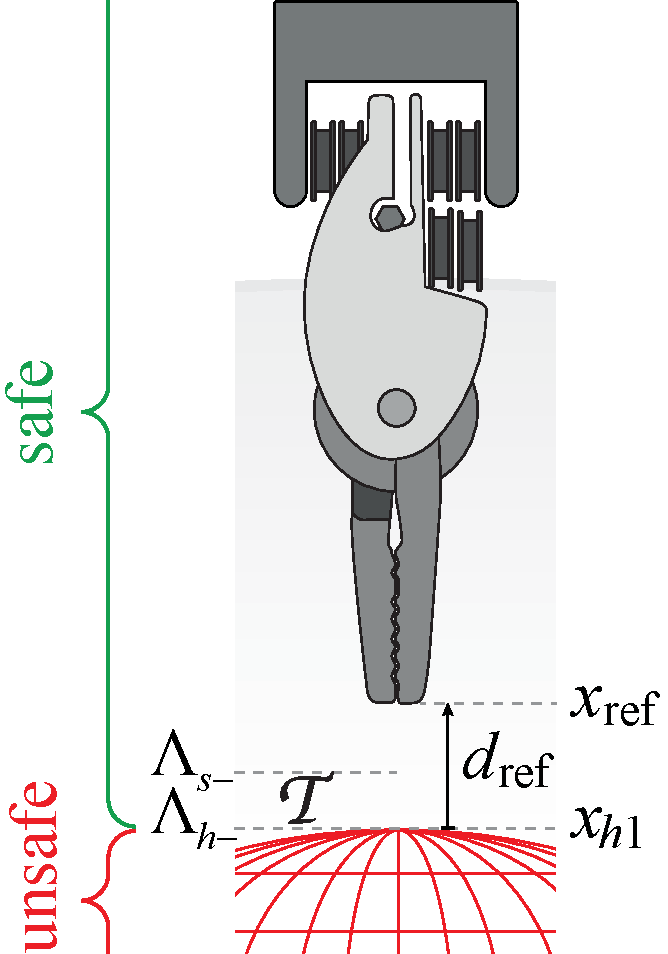
\includegraphics[height=4.2cm]{dynamic_boundary_limits.pdf}\label{fig:over_1}} \hspace{0.5cm}
\subbottom[Time sequence of a tool following a relative reference $d_\text{ref}$]{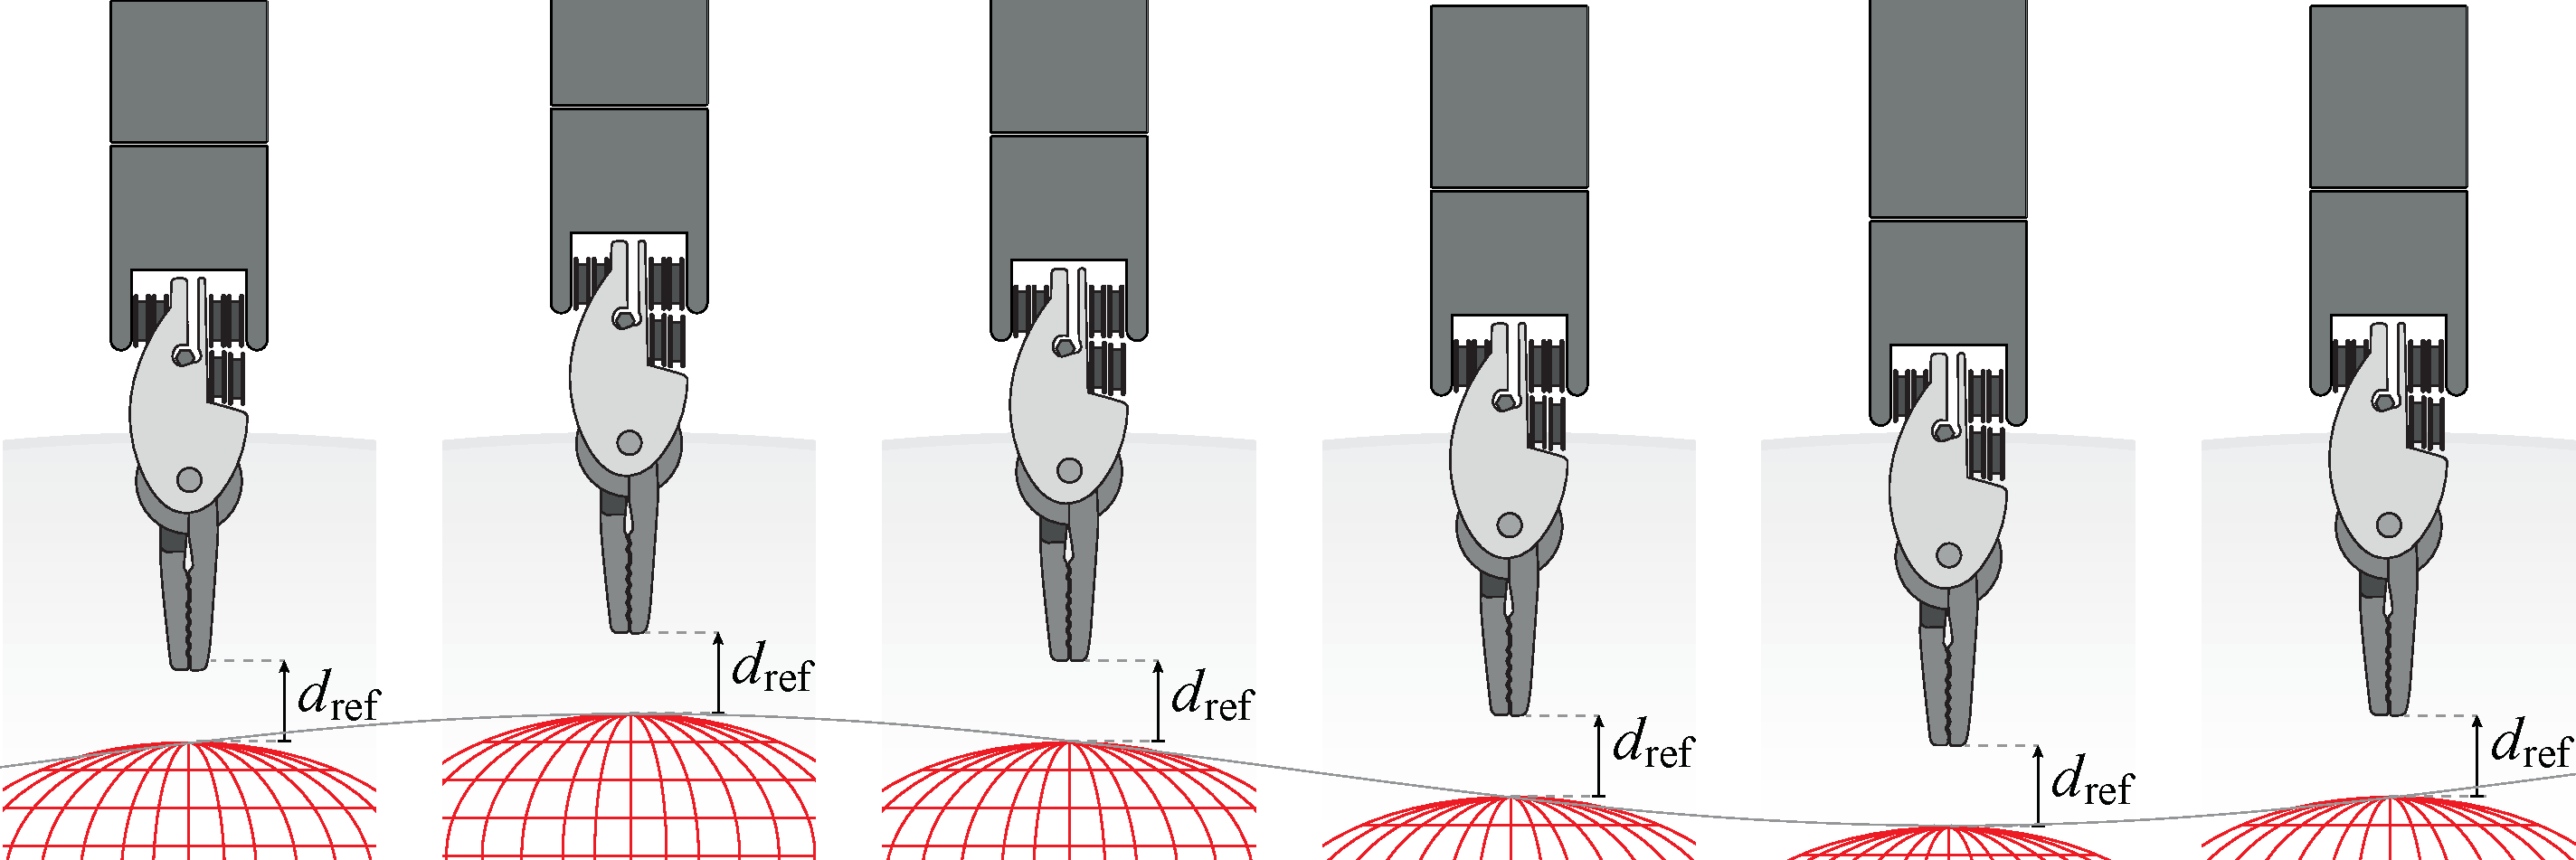
\includegraphics[height=4.2cm]{dynamic_boundary_sequence.pdf}\label{fig:over_2}}%
\caption{The objective is to control the distance to the object by following a relative reference $d_\text{ref}$, such that the surgeon experiences the object as static and can operate as if the object was in fact standing still. An overview of terms applied is found in \autoref{fig:over_1}.}
\label{fig:dynamic_overview}
\end{figure}
Thus a model of a beating heart will first be outlined.
%\begin{figure}[H]
%	\center
%		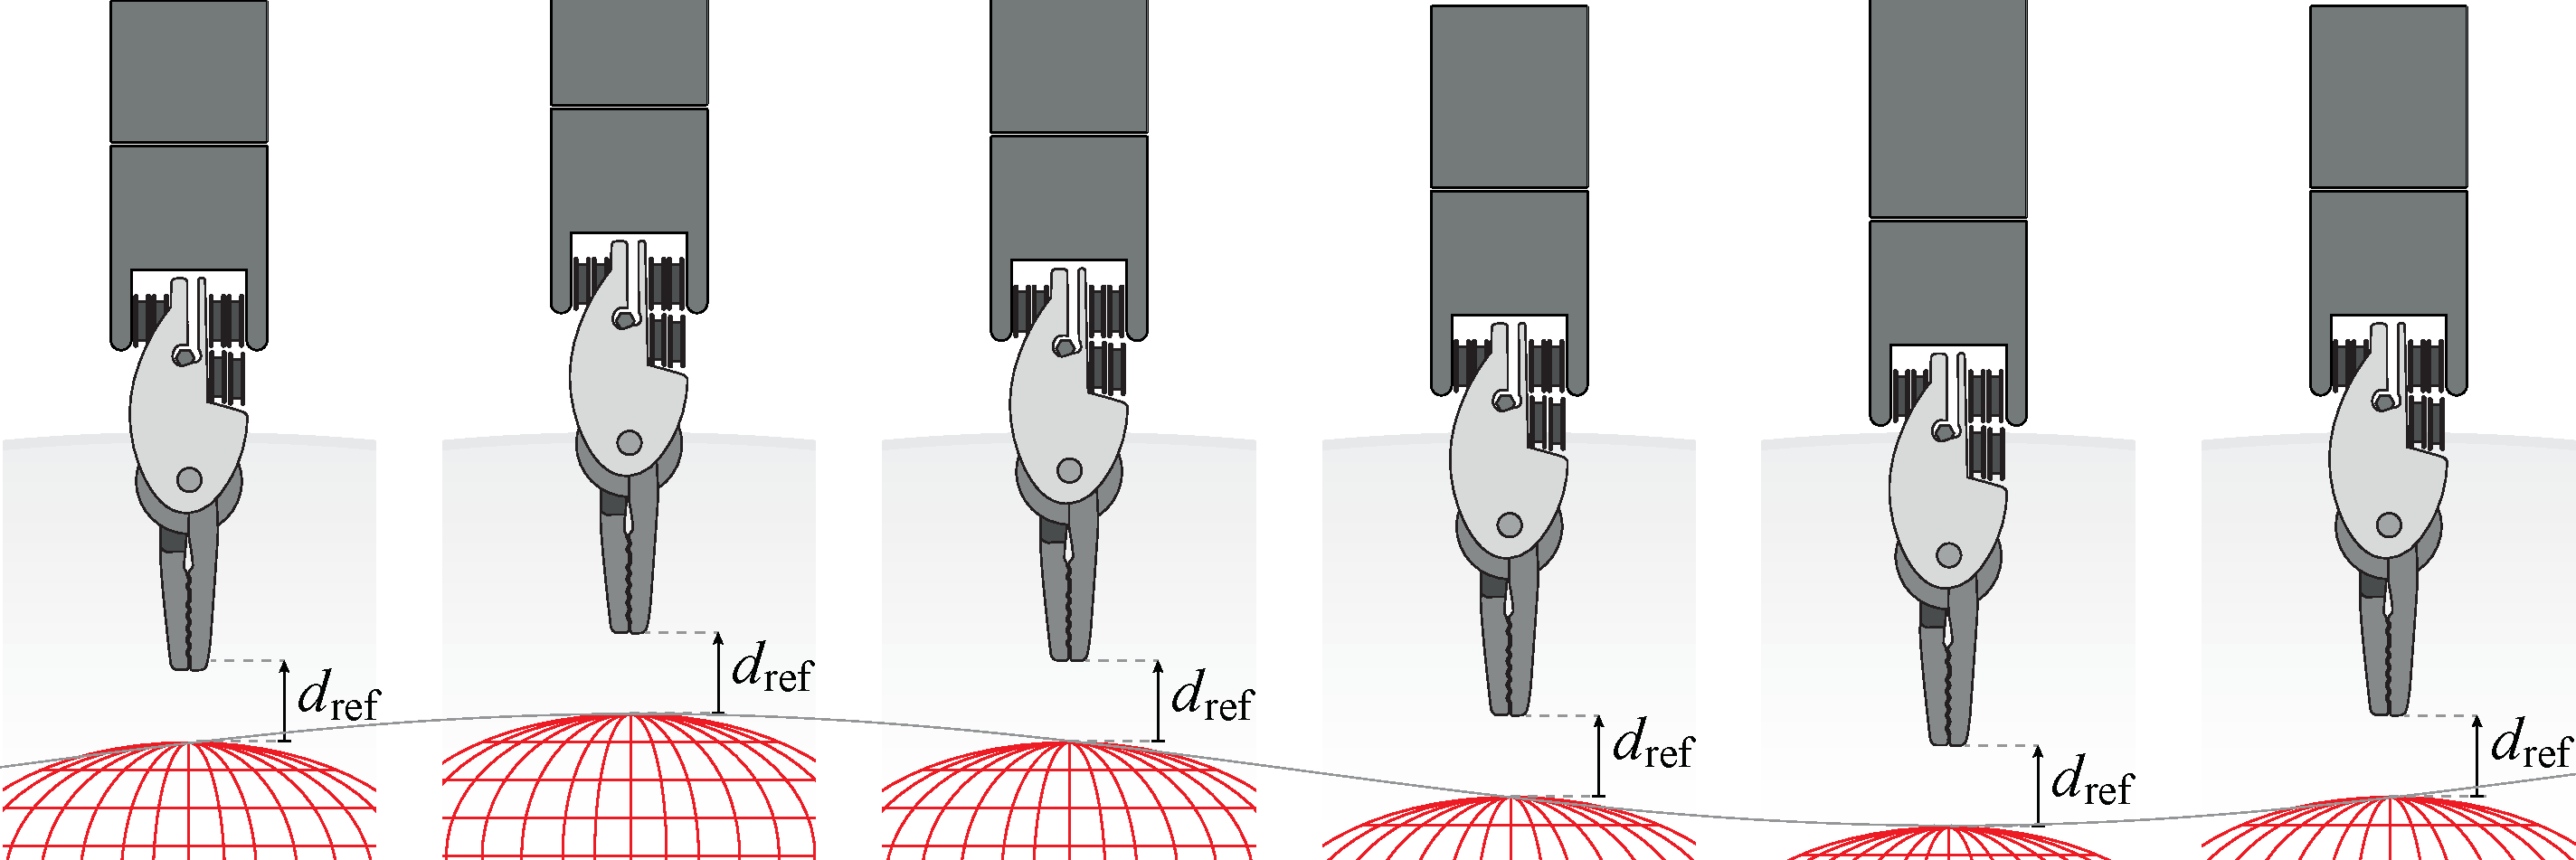
\includegraphics[width=1\textwidth]{dynamic_boundary_sequence.pdf}
%	\caption{lol.}
%	\label{fig:dynamic_overview}
%\end{figure}
%and..
%\begin{figure}[H]
%	\center
%		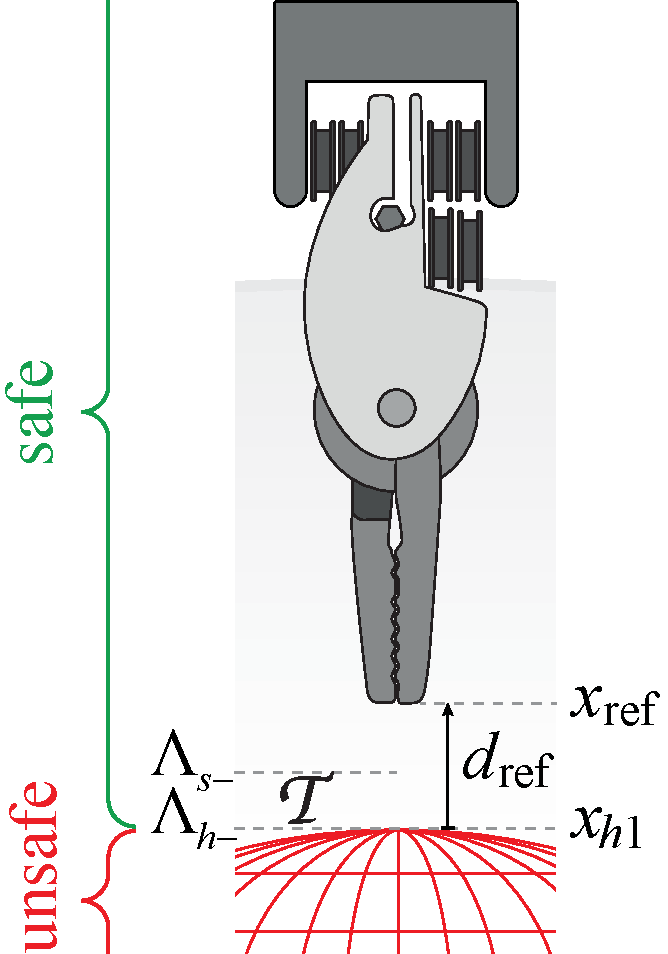
\includegraphics[width=0.2\textwidth]{dynamic_boundary_limits.pdf}
%	\caption{lol.}
%	\label{fig:dynamic_overview_2}
%\end{figure}
\subsubsection*{Modelling the Beating Heart}
\vspace{-2mm}
The simplified heart movement can be represented as a matrix with eigenvalues on the imaginary axis in the complex frequency domain:
\begin{flalign}
\dot{\textbf{x}}_h =
\dot{\begin{bmatrix}
x_{h1}\\x_{h2}
\end{bmatrix}} =
\begin{bmatrix}
0 & \omega_h \\ -\omega_h & 0
\end{bmatrix}
\begin{bmatrix}
x_{h1}\\x_{h2}
\end{bmatrix} \kk \text{with} \kk \mathbf{x}_{h}(0) =\begin{bmatrix}
x_{h10} \\
x_{h20}
\end{bmatrix}
\label{eq:beating_heart_sine}
\end{flalign}
\begin{tabular}{rp{14cm}} 
where  &  \\
$x_{h1}$& is the position of a point on the surface of the heart \\
$x_{h2}$& is the velocity of the point \\
$\omega_h$& is the heartbeat frequency, $\omega_h = 2\pi/T_h$ rad/s with an average heartbeat period $T_h=1.1$\,s \citep{bib:heart_berkeley} \\
$x_{h10}$ & is the initial value of $x_{h1}$ \\
$x_{h20}$ & is the initial value of $x_{h2}$\\
\end{tabular}\\


Note that the magnitude of $\omega_h$ determines the frequency and that the initial conditions determines the amplitude of the heart oscillation. The heartbeat will with this system have a natural oscillation around zero. 
\subsubsection*{Modelling the Robot Slide Movement}
\vspace{-1mm}
To model the one dimensional robot movement along the slide axis, the same system model can be used as presented in \autoref{eq:1storder_1D_ss}, i.e.:
\vspace{-3mm}
\begin{flalign}
\dot{x_1} = -\tau^{-1} x_1 + \tau^{-1} u
\label{eq:good_old}
\end{flalign}

\vspace{-1mm}
The one dimensional model is used to simplify the equations thus precluding complications at this stage. Additionally, the second order model merely proved few advantages in the form of elimination of the overshoot.
\vspace{-1mm}
\subsubsection*{Introducing a Dynamic Reference in the Model}
\vspace{-1mm}
To be able to guarantee that a given distance is maintained between the heart and the robot end effector, an additional state can be added the system. Thus, a new set of states is introduced representing the movement of the beating heart, the movement of the robot and a relative distance $d_\text{ref}$.
%\begin{flalign*}
%\textbf{x} = \begin{bmatrix}
%x_1 \\ x_{h1} \\ x_{h2} \\ d_\text{ref}
%\end{bmatrix}
%\end{flalign*}
Combining \autoref{eq:beating_heart_sine} and \autoref{eq:good_old} with the relative distance yields the below stated linear state space system: 
\vspace{-3mm}
\begin{flalign}
\dot{\textbf{x}}(t) &= \dot{\begin{bmatrix}
	x_1\\x_{h1}\\x_{h2}\\ d_\text{ref}
	\end{bmatrix}} =
\underbrace{\underbrace{\begin{bmatrix}
		-1/\tau & 0 & 0 & 0\\0 & 0 & \omega_h & 0 \\ 0 & -\omega_h & 0 & 0 \\ 0& 0 & 0 & 0
		\end{bmatrix}}_{\textbf{A}}
	\begin{bmatrix}
	x_1\\x_{h1}\\x_{h2}\\ d_\text{ref}
	\end{bmatrix}}_{f(\mathbf{x})}+ 
\underbrace{\underbrace{\begin{bmatrix}
		1/\tau \\ 0 \\ 0 \\ 0
		\end{bmatrix}}_{\textbf{B}}}_{g(\mathbf{x})} \tilde{u}(x) \\
		\mathbf{y}(t) &= \underbrace{\begin{bmatrix}
		1 & 0 & 0 & 0
		\end{bmatrix}}_\textbf{C} \textbf{x}(t)
\end{flalign}	
where the control law is introduced with the relative difference between robot position and heart position, i.e. $x_\text{ref} = x_{h1} + d_\text{ref}$ such that:
\vspace{-3mm}
\begin{flalign}
\tilde{u}(\mathbf{x}(t)) &= \bar{\mathbf{N}}x_\text{ref} - \mathbf{K}\,x_1 \nonumber\\
&= \bar{\mathbf{N}}\Big( x_{h1}(t)+ d_\text{ref} \Big)-\mathbf{K} x_1(t) \nonumber \\
%&= -\mathbf{K} x_1(t) + \bar{\mathbf{N}}x_{h1}(t) + \bar{\mathbf{N}} d_\text{ref}\nonumber \\
&= %\underbrace{
	\begin{bmatrix}
-\mathbf{K} & \bar{\mathbf{N}} & 0 & \bar{\mathbf{N}} 
\end{bmatrix}
%}_{\bar{\textbf{K}}} 
\textbf{x}(t) \nonumber\\
&= \bar{\textbf{K}} \textbf{x}(t)
\label{eq:utilde_dynamic}
\end{flalign}
\begin{tabular}{rl}
where &\\
$\tau$ & is the time constant of the first order system $\tau=0.11$\,s as given in \autoref{sec:model_slide}\\
$\mathbf{K}$ & is the linear system controller designed according to \autoref{eq:K_1}, $\mathbf{K} \in \mathbb{R}$ \\
$\bar{\textbf{N}}$ & is the system gain found according to \autoref{eq:barm_1}, $\bar{\mathbf{N}} \in \mathbb{R}$ \\
$\bar{\textbf{K}}$ & is the augmented feedback vector, $\bar{\textbf{K}} \in \mathbb{R}^{1 \times 4}$
\end{tabular}\\

%Such that:
%\begin{flalign}
%\tilde{u} = \bar{\textbf{K}} \textbf{x}
%\label{eq:utilde_dynamic}
%\end{flalign}
Note how the closed loop system can be rewritten in a more intuitive way, such that the system is reduced to three states taking $d_\text{ref}$ as input:
\vspace{-1mm}
\begin{flalign}
\dot{\begin{bmatrix}
	x_1\\x_{h1}\\x_{h2}\\d_\text{ref}
	\end{bmatrix}} &=
\underbrace{\underbrace{\begin{bmatrix}
		-1/\tau & 0 & 0 & 0\\0 & 0 & \omega_h & 0 \\ 0 & -\omega_h & 0 & 0 \\ 0& 0 & 0 & 0
		\end{bmatrix}}_{\textbf{A}}
	\begin{bmatrix}
	x_1\\x_{h1}\\x_{h2}\\d_\text{ref}
	\end{bmatrix}}_{f(\mathbf{x})}+ 
\underbrace{\underbrace{\begin{bmatrix}
		1/\tau \\ 0 \\ 0 \\ 0
		\end{bmatrix}}_{\textbf{B}}}_{g(\mathbf{x})}
\underbrace{\underbrace{\begin{bmatrix}
		-\mathbf{K} & \bar{\mathbf{N}} & 0 & \bar{\mathbf{N}}
		\end{bmatrix}}_{\bar{\textbf{K}}}
	\begin{bmatrix}
	x_1\\x_{h1}\\x_{h2}\\d_\text{ref}
	\end{bmatrix}}_{\tilde{u}(x)} \\
\dot{\begin{bmatrix}
	x_1\\x_{h1}\\x_{h2}
	\end{bmatrix}} &=
\underbrace{\begin{bmatrix}
	-(\mathbf{I}+\mathbf{K})/\tau & \bar{\mathbf{N}}/\tau & 0\\0 & 0 & \omega_h \\ 0 & -\omega_h & 0
	\end{bmatrix}}_{\textbf{A}_{cl}}
\begin{bmatrix}
x_1\\x_{h1}\\x_{h2}
\end{bmatrix}+ 
\underbrace{\begin{bmatrix}
	\bar{\mathbf{N}}/\tau \\ 0 \\ 0
	\end{bmatrix}}_{\textbf{B}_{cl}}
d_{ref}
\label{eq:cl_dynamic}
\end{flalign}
Note the eigenvalues of $\textbf{A}_{cl}$:
\vspace{-7mm}
\begin{flalign*}
\lambda_{\textbf{A}_{cl}} = \begin{cases}
-90 \\
5.71\,j \\
-5.71\,j
\end{cases}
\end{flalign*}
The eigenvalues reveal a stable (controllable) subsystem consisting of the robot end effector and an obviously marginally stable (uncontrollable) subsystem consisting of the beating heart.

This concludes the augmented system. Thus a \gls{cbf} will be constructed.
\vspace{-1mm}
\section{Construction of CBF}
\vspace{-3mm}
A barrier certificate for \autoref{eq:cl_dynamic} with a zero level set at the surface of the heart, comprises moving boundaries and hence should be a function of both robot and heart position. \Autoref{def:safety} implies that the \gls{cbf} should be constructed with unsafe region $\mathcal{X}_u$ below the surface of the heart, i.e. such that $B(x_1,x_{h1})$ is positive if $x_1<x_{h1}$ and negative otherwise. The coherence is clear:
\vspace{-1mm}
\begin{equation}
x_{h1} - x_1 > 0 \kk  \Rightarrow \kk \mathbf{x} \in \mathcal{X}_u \kk\Leftrightarrow\kk B(\mathbf{x}) > 0 \nonumber
%\\
%-x_1 + x_{h1} &> 0 \kk  \\
%x_{h1} - x_1 &> 0 
\end{equation}

\vspace{-2mm}
Thus a \gls{cbf} can be constructed as:
\vspace{-4mm}
\begin{flalign}
B(x_1,x_{h1})= \tilde{c}(x_{h1}-x_1)\label{eq:barrier_dynamic}
\end{flalign}

\vspace{-1mm}
with a positive constant $\tilde{c}>0$. Setting $\tilde{c} = 1$ yields a 1:1 mapping which indeed will be the case here. Thus according to \autoref{def:cbf} this is a valid CBF if $L_gB(\mathbf{x}) \neq 0$ and $\{\mathbf{x} \in \mathcal{X} | B( x_1 , x_{h1}) \leq 0 \} \neq \emptyset$. The latter  is trivial as the safe states are present if $d_\text{ref}>0$. Thus  $L_gB(x_1,x_{h1)}$ is analysed:
\begin{flalign}
L_gB(\mathbf{x}) = \frac{d B(x_1,x_{h1})}{ d \textbf{x}}g(\mathbf{x}) \Biggm|_{g(\mathbf{x}) = \textbf{B}}  
&= \begin{bmatrix}
\dfrac{\partial B(x_1,x_{h1})}{\partial x_1} & \dfrac{\partial B(x_1,x_{h1})}{\partial x_{h1}} & \dfrac{\partial B(x_1,x_{h1})}{\partial x_{h2}} & \dfrac{\partial B(x_1,x_{h1})}{\partial d_\text{ref}}
\end{bmatrix} \textbf{B} \nonumber \\
&= \begin{bmatrix}
-\tilde{c} & \tilde{c} & 0 & 0
\end{bmatrix}
\begin{bmatrix}
1/\tau\\
0 \\ 0 \\ 0
\end{bmatrix} \Bigm|_{\tilde{c}=1}  =
\frac{-1}{\tau} \neq 0 \quad \forall \, \mathbf{x} \in \mathcal{X}
\label{eq:lgb_dynamic}
\end{flalign}
It is seen that $L_gB(\mathbf{x}) \neq 0 \,\, \forall\,\, \mathbf{x} \in \mathcal{X}$. The \gls{cbf} is therefore valid on $\mathcal{X}$.
\section{Control Design}
The control law is, just as in \autoref{chap:cbf_1d_static}, split in two parts. A linear controller where no safety precautions are taken is used in $\mathcal{Y}$ and a controller ensuring safety is used in $\mathcal{T} \bigcup \mathcal{X}_u$. The controller ensuring safety is defined in \autoref{eq:control_law_safety}.

The transition between the two controllers in $\mathcal{T}$ is determined by $\sigma(\mathbf{x})$ which is defined in \autoref{eq:smoothness}. Thus a scalar $\epsilon$ is required. In this case, $\epsilon$ determines downright when the effect of the safety controller $k_0(\mathbf{x})$ is brought into effect, while the weighting of $k_0(\mathbf{x})$ is determined by $\sigma(\mathbf{x})$. To give the safety controller some margin to force the robot end effector away from $\mathcal{X}_u$, it is reasonable to let $k_0(\mathbf{x})$ take effect when the distance $d_\text{ref}$ reaches 1\,cm, thus:
\vspace{-3mm}
\begin{flalign}
\epsilon = 0.01\label{eq:epsilon_dynamic}
\end{flalign}

%\vspace{-3mm}
%Thus $\sigma(x)$ can be stated as:
%\begin{flalign}
%\sigma(x) = 
%\begin{cases}
%0 & \text{if} \mm B(x_1,x_{h1}) \leq -\epsilon \\
% -2  \left( \dfrac{B(x_1,x_{h1}}{\epsilon} \right)^3 - 3\left( \dfrac{B(x_1,x_{h1})}{\epsilon} \right)^2 +1  \kk &\text{if} \mm B(x_1,x_{h1}) \in (-\epsilon,0) \\
%1  &\text{if} \mm B(x_1,x_{h1}) \geq 0
%\end{cases}
%\label{eq:sig_dynamic}
%\end{flalign} 
The safety controller, as defined in \autoref{eq:control_law_safety}, requires  the Lie derivatives of the CBF, where $L_gB(\mathbf{x})$ is found in \autoref{eq:lgb_dynamic}, and $L_fB(\mathbf{x})$ is found as:
\begin{flalign}
L_fB(\mathbf{x}) &= \frac{dB(x_1,x_{h1})}{d\textbf{x}}f(\textbf{x})\Bigm|_{f(\textbf{x})=\textbf{A}\textbf{x}} \nonumber \\
&= \begin{bmatrix}
\dfrac{\partial  B(x_1,x_{h1})}{\partial x_1 } & \dfrac{\partial  B(x_1,x_{h1})}{\partial x_{1h} } & \dfrac{\partial  B(x_1,x_{h1})}{\partial x_{2h} } & \dfrac{\partial  B(x_1,x_{h1})}{\partial d_\text{ref} }
\end{bmatrix}  \begin{bmatrix}
1/\tau & 0 & 0 & 0 \\
0 & 0 & \omega_h & 0 \\
0 & -\omega_h & 0 & 0 \\
0 & 0 & 0 & 0 
\end{bmatrix} \begin{bmatrix}
x_1 \\ x_{x1} \\ x_{x2} \\ d_\text{ref}
\end{bmatrix} \nonumber \\
&=
\begin{bmatrix}
-\tilde{c} & \tilde{c} & 0 & 0
\end{bmatrix}
\begin{bmatrix}
-x_1/\tau\\
\omega_h x_{h2} \\
-\omega_h x_{h1} \\
0
\end{bmatrix} =
\tilde{c}\left(\omega_h x_{h2} + \frac{ x_1}{\tau}\right) \Bigm|_{\tilde{c}=1} = \omega_hx_{h2} + \dfrac{x_1}{\tau}
\label{eq:Lf_dynamic}
\end{flalign}

\begin{recap}[Control Law for Dynamic System with Relative Reference]
Using \autoref{eq:control_law}, the control law can be summarized as:
\begin{flalign*}
u(\mathbf{x}) = \sigma(\mathbf{x})k_0(\mathbf{x}) + (1-\sigma(\mathbf{x}))\tilde{u}(\mathbf{x})
\end{flalign*}
\begin{tabular}{rp{12.5cm}} 
where  &  \\
$\sigma(\mathbf{x})$ & is calculated from \autoref{eq:smoothness} with $B(\mathbf{x})$ found in \autoref{eq:barrier_dynamic} and $\epsilon$ found in \autoref{eq:epsilon_dynamic}\\
$k_0(\mathbf{x})$ & is calculated from \autoref{eq:control_law_safety} with the Lie derivatives from \ref{eq:lgb_dynamic} and \ref{eq:Lf_dynamic} \\
$\tilde{u}(\mathbf{x})$ & is calculated from \autoref{eq:utilde_dynamic}
\end{tabular}\\
\end{recap}
This completes the control design.

\section{MATLAB Results}
The results shown are implemented with the following characteristics:
\vspace{-2mm}
\begin{itemize}
	\itemsep-0.7mm
\item Extrapolation by means of forward Euler.
\item A sampling rate $f_s=2\,$kHz.
\item Simulation time for 5\,s.
\item The distance $d_\text{ref}$ is initially set to 3\,cm which is safe. At 2\,s the distance $d_\text{ref}$ is altered to -1\,cm emulating a surgeon who accidentally forced the robot to penetrate the heart. The expected outcome of this is obviously that the safety controller prevents this by ensuring a distance between end effector and the beating heart.
\item Initial conditions are set such that the robot end effector is positioned at a distance to the heart greater than the desired distance. The expected outcome is that the system will attempt to track the distance $x_1-x_{h1}=d_\text{ref}$.
\end{itemize}
The MATLAB implementation itself can be found in \autoref{app:slide_implement_1} and in \autoref{app:cd} under the path \texttt{matlab\_scripts/beating\_heart/beating\_heart\_controller.m}. The state trajectory is plotted in \autoref{fig:matlab_dynamics}.

\vspace{-2mm}
\begin{figure}[H]
	\center
		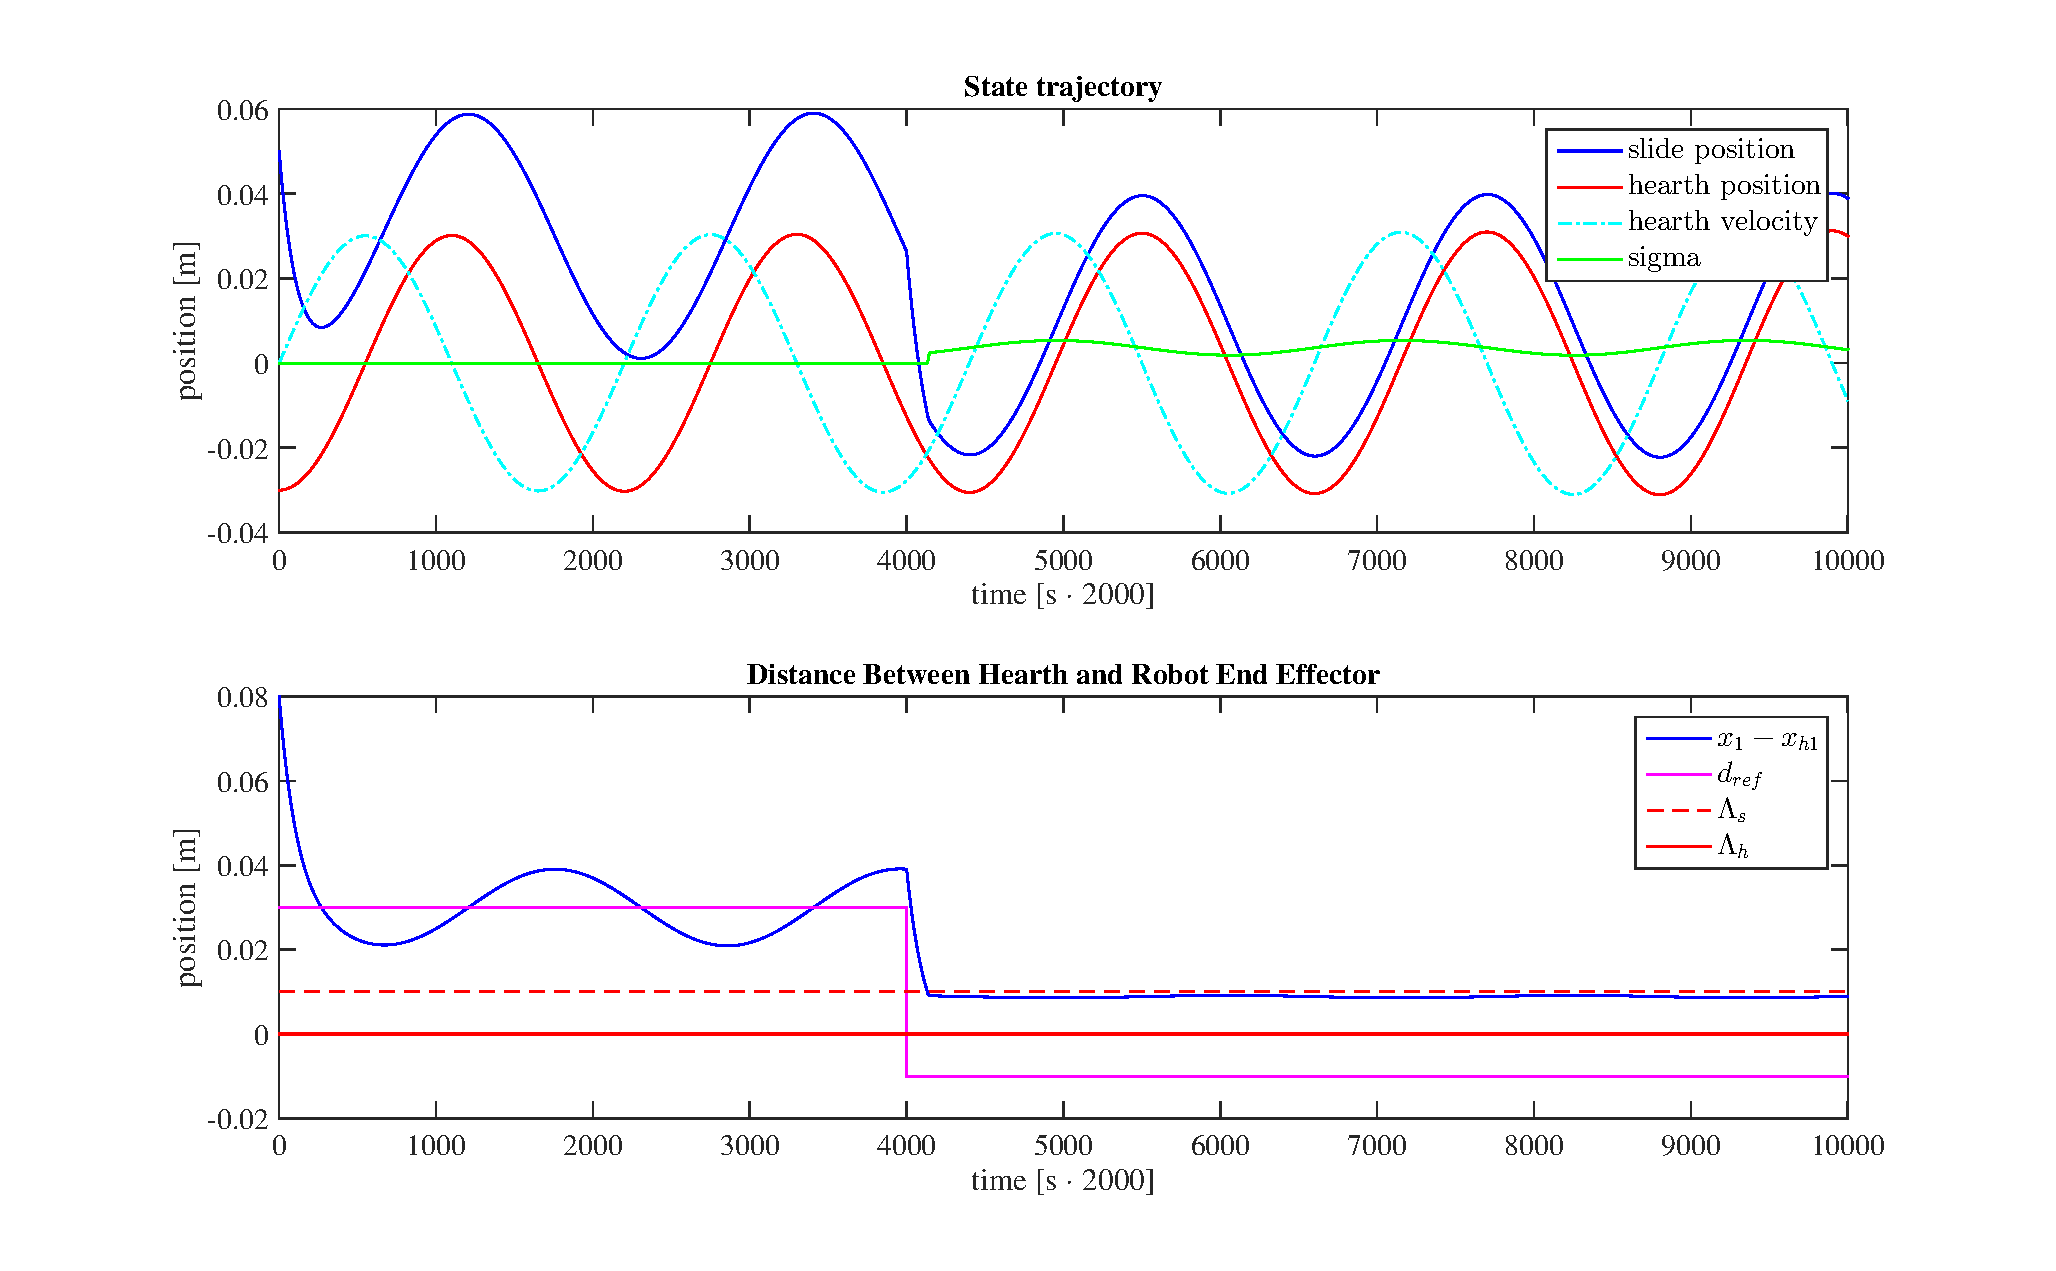
\includegraphics[width=1\textwidth]{state_trajectory_dynamic_matlab.eps}
	\caption{Dynamic system with heart position defined as the zero level set of the CBF. References are given as relative distances to the moving surface. When a reference outide the sage region is given, the safety controller prevents the tool from entering the unsafe region.}
    \label{fig:matlab_dynamics}
\end{figure}
It is from \autoref{fig:matlab_dynamics} seen that the robot end effector settles at a distance at $d_\text{ref}=3\,$cm until the simulation reaches 2\,s ($k=4000$). Then $d_\text{ref}$ changes to -1\,cm which causes the safety controller to react. The state $x_1$ settles at a safe distance from the beating heart which is left untouched, and the simulated controller is thereby verified to work as intended.

\section{Implementation on the Da Vinci Robot}

%\newpage
%%\begin{flalign}
%%f_{cl}(x)=\dot{\begin{bmatrix}
%%	x_1\\x_{h1}\\x_{h2}\\d_\text{ref}
%%	\end{bmatrix}} =
%%\underbrace{\underbrace{\begin{bmatrix}
%%		-1/\tau & 0 & 0 & 0\\0 & 0 & \omega_h & 0 \\ 0 & -\omega_h & 0 & 0 \\ 0& 0 & 0 & 0
%%		\end{bmatrix}}_{A}
%%	\begin{bmatrix}
%%	x_1\\x_{h1}\\x_{h2}\\d_\text{ref}
%%	\end{bmatrix}}_{f(x)}+ 
%%\underbrace{\underbrace{\begin{bmatrix}
%%		1/\tau \\ 0 \\ 0 \\ 0
%%		\end{bmatrix}}_{B}}_{g(x)}
%%\underbrace{\underbrace{\begin{bmatrix}
%%		-k & \bar{N} & 0 & \bar{N}
%%		\end{bmatrix}}_{K}
%%	\begin{bmatrix}
%%	x_1\\x_{h1}\\x_{h2}\\d_\text{ref}
%%	\end{bmatrix}}_{\tilde{u}(x)}
%%\end{flalign}
%%or formulated equivalently as
%%\begin{flalign}
%%\dot{\begin{bmatrix}
%%	x_1\\x_{h1}\\x_{h2}
%%	\end{bmatrix}} =
%%\underbrace{\begin{bmatrix}
%%	-(1+k)/\tau & \bar{N}/\tau & 0\\0 & 0 & \omega_h \\ 0 & -\omega_h & 0
%%	\end{bmatrix}}_{A_{cl}}
%%\begin{bmatrix}
%%x_1\\x_{h1}\\x_{h2}
%%\end{bmatrix}+ 
%%\underbrace{\begin{bmatrix}
%%	\bar{N}/\tau \\ 0 \\ 0
%%	\end{bmatrix}}_{B_{cl}}
%%d_{ref}
%%\end{flalign}
%%\begin{tabular}{rl}
%%where &\\
%%$\tau$ & is the time constant of the first order system $\tau=0.11$\,s as given in \autoref{sec:model_slide}\\
%%$k$ & is the linear system controller designed according to \autoref{eq:K_1}\\
%%$\bar{N}$ & is the system gain found according to \autoref{eq:barm_1}
%%\end{tabular}\\
%
%
%
%%
%%where $x_{h1}$ is the position of a point on the surface of the heart and $x_{h2}$ is the velocity of the point.
%%Here $\omega_h$ represents the frequency of the heart, 
%%$\omega_h$ has an average heartbeat period of 1.1\,s \citep{bib:heart_berkeley}, 
%%$\omega_h$ is set to be $2\pi/1.1$. 
%%In \autoref{fig:1stordersys_dynamiclimits} the moving surface of the heart is plotted over time, offset to an axis of oscillation in -6\,cm relative to the slide position. This curve marks the boundary to the unsafe region below it, and crossing this curve (from the safe region above it) corresponds to penetrating the heart surface with the surgical instrument tip. Note that the flexibility of the surface of the heart, at contact with the rigid tool, is not considered in the scope of this thesis. 
%%
%%\begin{figure}[htbp]
%%	\centering
%%	\includegraphics[width=0.65\textwidth]{1stordersys_dynamiclimits.pdf}
%%	\caption{Example of a moving surface representing the heart, marking the boundary to the unsafe region $\mathcal{X}_u$. A reference is set within the safe region as a fixed distance to the surface of the beating heart.}
%%	\label{fig:1stordersys_dynamiclimits}
%%\end{figure}
%%
%%In \autoref{fig:1stordersys_dynamiclimits} a sine amplitude of 2\,cm is used and the time dependent reference for the robot tool tip is defined as the heart position plus a fixed distance of 1\,cm in the positive slide direction $x_\text{ref}=x_{h1}+d_\text{ref}$, i.e. according to \autoref{eq:utilde} the linear position controller to be used in $\mathcal{X}_0$ is
%%\begin{equation}
%%\tilde{u}(t) = \bar{N}(x_{h1}(t)+d_\text{ref})-Kx(t) \label{eq:utilde_dynamic}
%%\end{equation}
%%\textcolor{red}{Or should it be $-k_1x_1$ no matter the order of the system?}
%%The reference distance can be picked as any nonnegative value still allowing the slide position to stay within its (upper) physical limit.
%The dynamic surface representing the heart also put forth new requirements to the safety controller, as the boundary between the safe and unsafe regions $\mathcal{X}_0$ and $\mathcal{X}_u$ (and thereby also the transition region $\mathcal{T}$ between the use of linear and safety controller) is now moving concurrently with the heart surface. This requires the construction of barrier certificates that are functions of robot state as well as the dynamic surface position.
%
%
%
%\section{Safe Controller Design for First Order System}
%First a linear position controller is designed for the augmented system consisting of the first order system modelled in \autoref{subsec:model_1d} and the simplified heart model in \autoref{eq:beating_heart_sine}. The controller is designed on the form presented in \autoref{eq:utilde}, and for the dynamic system, the reference is designed to be a fixed distance to the surface of the heart, as described in \autoref{eq:utilde_dynamic}.
%
%Once the closed-loop system has been designed, a barrier certificate is constructed iteratively by formulating a function that has its (dynamic) zero level set coinciding with the surface position of the heart, and is positive (indicating the unsafe region $\mathcal{X}_u$) below the surface and negative above, thus conforming with the first two requirements for a barrier certificate as given by \autoref{def:barrier_certificate}.
%
%In order to test compliance with the third requirement for a barrier certificate, the candidate barrier function is tested with the designed linear first order system according to the requirement in \autoref{req2}, and the candidate barrier function is altered iteratively until this requirement is fulfilled.
%
%When a barrier certificate for the closed-loop system has been found, a safety controller is designed according to \autoref{eq:control_law_safety}, and the region $\mathcal{T}$ is defined by choosing the constant $\epsilon$ and using the bump function $\sigma(x)$ in \autoref{eq:smoothness}, arriving at the safe controller in \autoref{eq:control_law} employing the linear position controller on $\mathcal{X}_0\setminus\mathcal{T}$ and the linear combination of the position controller and the CBF on $\mathcal{T}$
%
%\subsection{Setting up the Closed-Loop System and Designing the Linear Controller}
%An augmented state-space model including the dynamics of the robot tool from \autoref{eq:1storder_1D_ss} as well as the beating heart from \autoref{eq:beating_heart_sine}, is set up for the closed-loop first order system
%\begin{equation}
%f_{cl}(x)=\dot{\begin{bmatrix}
%	x_1\\x_{h1}\\x_{h2}\\d_\text{ref}
%	\end{bmatrix}} =
%\underbrace{\underbrace{\begin{bmatrix}
%		-1/\tau & 0 & 0 & 0\\0 & 0 & \omega_h & 0 \\ 0 & -\omega_h & 0 & 0 \\ 0& 0 & 0 & 0
%		\end{bmatrix}}_{A}
%	\begin{bmatrix}
%	x_1\\x_{h1}\\x_{h2}\\d_\text{ref}
%	\end{bmatrix}}_{f(x)}+ 
%\underbrace{\underbrace{\begin{bmatrix}
%		1/\tau \\ 0 \\ 0 \\ 0
%		\end{bmatrix}}_{B}}_{g(x)}
%\underbrace{\underbrace{\begin{bmatrix}
%		-k & \bar{N} & 0 & \bar{N}
%		\end{bmatrix}}_{K}
%	\begin{bmatrix}
%	x_1\\x_{h1}\\x_{h2}\\d_\text{ref}
%	\end{bmatrix}}_{\tilde{u}(x)}
%\end{equation}
%or formulated equivalently as
%\begin{equation}
%\dot{\begin{bmatrix}
%	x_1\\x_{h1}\\x_{h2}
%	\end{bmatrix}} =
%\underbrace{\begin{bmatrix}
%	-(1+k)/\tau & \bar{N}/\tau & 0\\0 & 0 & \omega_h \\ 0 & -\omega_h & 0
%	\end{bmatrix}}_{A_{cl}}
%\begin{bmatrix}
%x_1\\x_{h1}\\x_{h2}
%\end{bmatrix}+ 
%\underbrace{\begin{bmatrix}
%	\bar{N}/\tau \\ 0 \\ 0
%	\end{bmatrix}}_{B_{cl}}
%d_{ref}
%\end{equation}
%\begin{tabular}{rl}
%where &\\
%$\tau$ & is the time constant of the first order system $\tau=0.11$\,s as given in \autoref{sec:model_slide}\\
%$k$ & is the linear system controller designed according to \autoref{eq:K_1}\\
%$\bar{N}$ & is the system gain found according to \autoref{eq:barm_1}
%\end{tabular}\\
%
%\textcolor{red}{Should we design a $k$ that is slower conforming with what is found to be implementable?}
%
%Before designing the controller $k$, the stability of this system is analysed. \textcolor{red}{Be sure it's the same for reference as for estimated state!} In order for the system to be (asymptotically) stable, the error should converge to zero
%\begin{equation}
%e(t)=x_\text{ref}(t)-x_1(t)=x_{h1}(t)+d_\text{ref}-x_1(t) = 0 \label{eq:ref_error}
%\end{equation}
%The requirement of the system being stable can be tested as the derivative of the error converging to zero
%\vspace{-5mm}
%\begin{subequations}
%\begin{align}
%\dot{e}(t)=\dot{x}_\text{ref}(t)-\dot{x}_1(t)=\dot{x}_{h1}(t)-\dot{x}_1(t)
%&= \omega_h x_{h2}(t) - (-\tfrac{1}{\tau}x_1(t)+\tfrac{1}{\tau}\bar{N}x_\text{ref}(t-\tfrac{1}{\tau}kx_1(t)) \nonumber\\
%&= \omega_h x_{h2}(t) + \tfrac{1}{\tau}(1+k)x_1(t)-\tfrac{1}{\tau}\bar{N}x_\text{ref}(t)
%\end{align}
%For a first order system of this particular configuration of the $A$ and $B$ matrices, as seen from \autoref{eq:barm_1}, $\bar{N}=1+k$, reducing the equation to
%\begin{equation}
%\dot{e}(t) =\omega_h x_{h2}(t) + \tfrac{1}{\tau}\bar{N}(x_1(t)-x_\text{ref}(t) = \omega_h x_{h2}(t) - \tfrac{1}{\tau}\bar{N}e(t)
%\end{equation}
%Now setting the error derivative equal to zero
%\begin{align}
%0 &= \omega_h x_{h2}(t) - \tfrac{1}{\tau}\bar{N}e(t)\nonumber\\
%\tfrac{1}{\tau}\bar{N}e(t) &= \omega_h x_{h2}(t)\nonumber\\
%e(t) &= \frac{\omega_h \tau}{\bar{N}}x_{h2}(t)
%\end{align}
%The value of $x_{h2}$ is time dependent, but will have its maximum and minimum values in the amplitude of the sine, i.e. for a heart sine amplitude of $A_\text{heart}=2$\,cm $x_{h2}\in[-0.02,0.02]$\,m.
%\end{subequations}
%This means that the error will fluctuate between the values
%\begin{equation}
%e(t) \in \begin{bmatrix} -\frac{\omega_h \tau}{\bar{N}}A_\text{heart},  & \frac{\omega_h \tau}{\bar{N}}A_\text{heart}  \end{bmatrix}
%\end{equation}
%\textcolor{red}{Makes no sense! How can the error derivative be zero only when the error is fluctuating?!}
%From safety, $x_1$ should always be above $x_{h1}$, i.e.
%\begin{equation}
%x_1(t)\geq x_{h1}(t) \qquad \Leftrightarrow \qquad x_{h1}(t)-x_1(t)\leq 0
%\end{equation}
%and as seen from \autoref{eq:ref_error}, this puts up a safety requirement for the reference distance
%\begin{equation}
%x_{h1}(t)-x_1(t) = e(t)-d_\text{ref}\leq 0 \qquad \Leftrightarrow \qquad d_\text{ref}\geq e_\text{max}=\frac{\omega_h \tau}{\bar{N}}A_\text{heart}
%\end{equation}
%
%Stability analysis: test that the system has negative poles, i.e. that all $\lambda$s are negative for which
%\begin{equation}
%\det\begin{vmatrix}
%A_{cl}-\lambda I & B_{cl}\\C_{cl}&D_{cl}
%\end{vmatrix}=0
%\end{equation}
%As the output should be the robot tool position, i.e. $C_{cl}=[1\,\,\,0\,\,\,0]$ and $D_{cl}=0$, this is found as
%\begin{align}
%&\det\begin{vmatrix}
%-(1+k)/\tau-\lambda & \bar{N}/\tau & 0 & \bar{N}/\tau\\
%0 & -\lambda  & \omega_h  & 0\\ 
%0 & -\omega_h & -\lambda & 0\\
%1 & 0 & 0 & 0
%\end{vmatrix}
%= 
%%(-(1+k)/\tau-\lambda) \cdot
%%\begin{vmatrix}
%%-\lambda  & \omega_h  & 0\\ 
%%-\omega_h & -\lambda & 0\\
%%0 & 0 & 0
%%\end{vmatrix}
%-1 \cdot \det\begin{vmatrix}
%\bar{N}/\tau & 0 & \bar{N}/\tau\\
%-\lambda & \omega_h  & 0\\ 
%-\omega_h & -\lambda & 0\\
%\end{vmatrix} \nonumber\\
%&\phantom{det}= -1\cdot \frac{\bar{N}}{\tau} \cdot \det 
%\begin{vmatrix}
%-\lambda & \omega_h\\
%-\omega_h &  -\lambda\\
%\end{vmatrix}
%= -\frac{\bar{N}}{\tau} \cdot (\lambda^2 +\omega_h^2)
%= 0 \qquad \Leftrightarrow \qquad \lambda = \pm\omega_h
%\end{align}
%\textcolor{red}{Not stable! positive eigenvalue in $\omega_h$}
%
%\subsection{Constructing a Control Barrier Function}
%As mentioned, a barrier certificate for this system with a zero level set at the surface of the heart, comprises moving boundaries and hence should be a function of both robot and heart position. According to \autoref{def:safety} a $B(x_1,x_{h1})$ should be constructed with unsafe region $\mathcal{X}_u$ below the surface of the heart, i.e. such that $B(x_1,x_{h1})$ is positive if $x_1<x_{h1}$ and negative otherwise. The very simplest function satisfying this requirement is a function
%\begin{equation}
%B_0(x_1,x_{h1})= c(x_{h1}-x_1)
%\end{equation}
%with a positive constant $c>0$. This would result in the Lie derivatives % $L_{f_{cl}}B_0(x)$
%\begin{subequations}
%\begin{align}
%L_fB_0(x) &= \frac{dB_0(x)}{dx}f(x) =
%\begin{bmatrix}
%-c & c & 0 & 0
%\end{bmatrix}
%\begin{bmatrix}
%-x_1/\tau\\
%\omega_h x_{h2} \\
%-\omega_h x_{h1} \\
%0
%\end{bmatrix}=
%c\left(\omega_h x_{h2} + \frac{ x_1}{\tau}\right)\\
%L_gB_0(x) &= \frac{dB(x)}{dx}g(x) =
%\begin{bmatrix}
%-c & c & 0 & 0
%\end{bmatrix}
%\begin{bmatrix}
%1/\tau\\
%0 \\ 0 \\ 0
%\end{bmatrix}=
%\frac{-c}{\tau}\\
%L_{f_{cl}}B_0(x) & 
%%=\frac{dB_0(x)}{dx}f_{cl}(x) 
%= L_fB_0(x)+L_gB_0(x)u = 
%%\begin{bmatrix}
%%	-c & c & 0 & 0
%%\end{bmatrix}
%%\begin{bmatrix}
%%\frac{\bar{N}(x_{h1}+d_{ref})-(1+k) x_1}{\tau} \\
%%\omega_h x_{h2} \\
%%-\omega_h x_{h1}
%%\end{bmatrix}=
%c\left(\omega_h x_{h2} - \frac{\bar{N}(x_{h1} + d_{ref})-(1+k) x_1}{\tau}\right)
%\end{align}
%\end{subequations}
%The Lie derivative $L_{f_{cl}}B_0(x)$ (with the heart sine placed as in \autoref{fig:1stordersys_dynamiclimits}) should be negative for  $x_1\in[-0.1,0.1]$, $x_{h1}\in [-0.08,-0.04]$ and $x_{h2}\in [-0.02,0.02]$. We thus require that (recall from \autoref{eq:barm_1} that $\bar{N}=K+1$ for the present first order system)
%\begin{align}
%\omega_h x_{h2} &< \frac{\bar{N}(x_{h1} + d_{ref})-(1+k) x_1}{\tau} = \frac{1+k}{\tau}(x_{h1} + d_{ref}-x_1)\nonumber\\
%\omega_h x_{h2} \frac{\tau}{1+k} &< x_{h1} + d_{ref}-x_1
%\end{align}
%With the largest positive value of $x_{h2}=0.02$\,m and the same controller $K=9$ is used as in \autoref{eq:K_1}, the left-hand expression attains a largest value of 0.00126\,m, requiring that the error between the robot tool position and the reference position always be slightly larger than a millimeter. 
%%2*pi/1.1*0.02/(10/0.11)
%%0.001256637061436
%Obviously this barrier function is not valid, and a different function is opted for.
%
%According to \cite{bib:org_control} a barrier certificate might be found iteratively by using $B_0(x)$ in the construction of a barrier certificate on the form
%\begin{equation}
%B(x) = 
%\begin{cases}
%B_0(x) & \text{if}\quad L_fB_0(x) \leq -\beta\\
%B_0(x)+\alpha(L_fB_0(x)+\beta)^2 & \text{if}\quad L_fB_0(x)>-\beta 
%\end{cases}
%\end{equation}
%where $\alpha>0$, $\beta>0$ are parameters to be determined. For the presented system this gives the barrier candidate function 
%\begin{equation}
%B(x) = 
%\begin{cases}
%c(x_{h1}-x_1) & \text{if}\quad c\left(\omega_h x_{h2} +  x_1/\tau\right) \leq -\beta\\
%c(x_{h1}-x_1)+\alpha(c\left(\omega_h x_{h2} +  x_1/\tau\right)+\beta)^2 & \text{if}\quad c\left(\omega_h x_{h2} +  x_1/\tau\right)>-\beta 
%\end{cases}
%\end{equation}
%\textcolor{red}{The constant $c$ is unimportant. Set $c=1$.  In the example in \citep{bib:org_control} they chose $\alpha=1/20$ and $\beta=1$, giving}
%\begin{equation}
%B(x) = 
%\begin{cases}
%x_{h1}-x_1 & \text{if}\quad x_1 \leq -0.11-0.2\pi x_{h2}\\
%x_{h1}-x_1+\dfrac{1}{20}\left(\dfrac{0.2\pi\,\, x_{h2} +   x_1}{0.11}+1\right)^2 & \text{if}\quad x_1 > -0.11-0.2\pi x_{h2} 
%\end{cases}
%\end{equation}
%\textcolor{red}{Need to test this!}
%
%
%\section{Safe Controller Design for Second Order System}
%\textcolor{red}{introduce}
%
%\subsection{Setting up the Closed-Loop System and Designing the Linear Controller}
%As for the first order system, the second order system in \autoref{eq:2ndorder_1D_ss} is augmented with the dynamics of the beating heart and with the reference given as a fixed distance from the surface of the beating heart
%\begin{equation}
%\dot{\begin{bmatrix}
%x_1\\x_2\\x_{h1}\\x_{h2}
%\end{bmatrix}} = \begin{bmatrix}
%0 & 1 & 0 & 0\\
%-\omega_n^2(1+k_1)  & -2\zeta \omega_n-\omega_n^2 k_2  & \omega_n^2\bar{N} & 0\\
%0 & 0 & 0 & \omega_h \\
%0 & 0 & -\omega_h & 0
%\end{bmatrix}\begin{bmatrix}
%x_1\\x_2\\x_{h1}\\x_{h2}
%\end{bmatrix} + \begin{bmatrix}
%0\\\omega_n^2\bar{N} \\ 0 \\ 0
%\end{bmatrix}d_{ref}
%\end{equation}
%\begin{tabular}{rl}
%where &\\
%$\omega_n$ & is the natural frequency of the second order system $\omega_n=17$\,rad/s as given in \autoref{sec:model_slide}\\
%$\zeta$ & is the damping ratio of the second order system $\zeta=0.05$ as given in \autoref{sec:model_slide}\\
%$[k_1\,\,\,k_2]$ & is the linear system controller designed according to \autoref{eq:K_2}\\
%$\bar{N}$ & is the system gain found according to \autoref{eq:Nbar_2}
%\end{tabular}\\
%
%
%Can also be written on augmented form where the reference is part of the state
%\begin{equation}
%\dot{\begin{bmatrix}
%	x_1\\x_2\\x_{h1}\\x_{h2}\\d_{ref}
%	\end{bmatrix}} = 
%\underbrace{\underbrace{\begin{bmatrix}
%		0 & 1 & 0 & 0 & 0\\
%		-\omega_n^2  & -2\zeta \omega_n  & 0 & 0 & 0\\
%		0 & 0 & 0 & \omega_h & 0\\
%		0 & 0 & -\omega_h & 0 & 0\\
%		0 & 0 & 0 & 0 & 0
%		\end{bmatrix}}_{A}
%	\begin{bmatrix}
%	x_1\\x_2\\x_{h1}\\x_{h2}\\d_{ref}
%	\end{bmatrix}}_{f(x)} + 
%\underbrace{\underbrace{\begin{bmatrix}
%		0\\\omega_n^2 \\ 0 \\ 0 \\ 0
%		\end{bmatrix}}_{B}}_{g(x)}
%\underbrace{\underbrace{\begin{bmatrix}
%		-k_1 & -k_2 & \bar{N} & 0 & \bar{N}
%		\end{bmatrix}}_{K}
%	\begin{bmatrix}
%	x_1\\x_2\\x_{h1}\\x_{h2}\\d_{ref}
%	\end{bmatrix}}_{u}
%\end{equation}
\chapter{3D System with Static Boundaries}\label{chap:cbf_3d_static}
now for full robot hand, describe kinematics and inverse kinematics solver!

\section{Safe Controller Design for First Order System}

\section{Safe Controller Design for Second Order System}
\chapter{3D System with Dynamic Boundaries} \label{chap:cbf_3d_dynamic}
probably there won't be time enough to do this, but in case there is it will still be with "heart" movement being sinus from Simon's controlled platform, it will not be possible to extend to the heart model from the paper

\section{Safe Controller Design for First Order System}

\section{Safe Controller Design for Second Order System}

\part[Controller Safety Verification with Putinar's Positivstellensatz]{Controller Safety Verification with \\Putinar's Positivstellensatz}\label{part:putinar}  % Title in square brackets is what goes in TOC
\chaptermark{Controller Safety Verification with Putinar's Positivstellensatz} % Running footer, here we do not want a line break
\chapter{Putinar's Positivstellensatz}\label{chap:putinar}
	Barrier certificates can be used to (in)validate the safety compliance of a controller design by testing if a barrier certificate can be found according to \autoref{eq:barrier_constraints} for the closed-loop system $f_{cl}(x)$. This can be done using Putinar's Positivstellensatz to define the spaces $\mathcal{X}$, $\mathcal{X}_u$ and $\mathcal{X}_0$ with \gls{sos} polynomials. 

A Positivstellensatz is a structure theorem of a positive (\gls{sos}) polynomial on some set, and gives an algebraic certificate that a solution exists for a system of real polynomial inequalities \citep{bib:positivstellensatz}. 

\textbf{Stengle's Positivstellensatz}: Given 
\begin{align}
\text{polynomials} \qquad & g_1,...,g_m \in \mathbb{R}[x]\\
\text{set} \qquad & g_J\equiv\prod_{j\in J} \text{ for } J\subseteq\{1...m\}, \text{ with } g_0\equiv 1
\end{align}
The set 
\begin{equation}
T(g_1,...,g_m)\equiv\{\sum\limits_{J\subseteq \{1...m\}}^{}u_Jg_J | u_J\in\Sigma\}
\end{equation} 
is called a preordering on $\mathbb{R}[x]$ generated by $g_1,...,g_m$. 

Theorem: for
\begin{align}
\text{set}	 \qquad & \mathbb{K}=\{x\in \mathbb{R}^n | g_i(x)\geq0\}, i=1...m\\
\text{polynomial} \qquad & p\in\mathbb{R}[x]
\end{align}
then
\begin{align}
p>0 \text{ on } \mathbb{K} & \Leftrightarrow pf=1+g \text{ for some } f,g\in T(g_1,...,g_m)\\
p\geq 0 \text{ on } \mathbb{K} & \Leftrightarrow  pf=p^{2k}+g \text{ for some } f,g\in T(g_1,...,g_m) \text{ and } k\in \mathbb{N}\\
p=0 \text{ on } \mathbb{K} & \Leftrightarrow -p^{2k}\in T(g_1,...,g_m) \text{ for some }  k\in \mathbb{N}
\end{align}
\citep{bib:sos_putinar_laurent}

Theorem: let $k$ be a real closed field,
\begin{align}
\text{polynomial} \qquad & f\in k[x]\\
\text{set}	 \qquad & \mathbb{K}=\{x\in k^n | f_j(x)\geq0, j=1...m\}
\end{align}
define 
\begin{equation}
P(f_1,...,f_m)\equiv \{\sum\limits_{J\subseteq\{i...m\}}^{} q_Jf_J: q_J\in \Sigma[x] \}
\end{equation}
where $\Sigma$ denotes a \gls{sos} variable and $\Sigma[x]$ denotes a polynomial \gls{sos} variable. Then
\begin{align}
\text{Nichtnegativstellensatz:} \qquad\qquad\quad &\nonumber\\
f\geq 0 \text{ on } \mathbb{K} \quad & \textup{ iff } \exists \ell \in \mathbb{N} \textup{ and } g,h\in P(f_1,...,f_m) \text{ such that } fg=f^{2\ell}+h\\
\text{Positivstellensatz:} \qquad\qquad\quad &\nonumber\\
f>0  \text{ on } \mathbb{K} \quad & \textup{ iff } \exists g,h\in P(f_1,...,f_m) \text{ such that } fg=1+h\\
\text{Nullstellensatz:} \qquad\qquad\quad &\nonumber\\
f=0 \text{ on } \mathbb{K} \quad & \textup{ iff } \exists \ell \in \mathbb{N} \textup{ and } g\in P(f_1,...,f_m) \text{ such that } f^{2\ell}+g=0
\end{align}

\citep{bib:sos_putainar_lasserre}

\textbf{Schm\"{u}dgen's Positivstellensatz}: Given
\begin{align}
\text{polynomial} \qquad & p\in\mathbb{R}[x]\\
\text{set} \qquad & \mathbb{K}=\{x\in \mathbb{R}^n | g_i(x)\geq0\}, i=1...m
\end{align}
then
\begin{equation}
p>0 \text{ on } \mathbb{K} \Rightarrow p\in T(g_1,...,g_m)
\end{equation}
\citep{bib:sos_putinar_laurent}

Provide simple characterization of polynomial polysive on a compact basic semialgebraic set $\mathbb{K}$. Let
\begin{equation}
(g_j)_{j=1}^m \subset \mathbb{R}[x]
\end{equation}
be such that the semialgebraic set
\begin{equation}
\mathbb{K}\equiv\{x\in\mathbb{R}^n: g_j(x)\geq 0, j=1...m\}
\end{equation}
is compact. If the polynomial $f\in\mathbb{R}[x]$ is strictly positive on $\mathbb{K}$, then
\begin{equation}
f\in P(f_1,...,f_m)
\end{equation}
that is
\begin{equation}
f = \sum\limits_{J\subseteq\{1...m\}}^{}f_Jg_J \quad \textup{for some SOS } f_J\in\Sigma[x], \textup{ with } g_J=\prod\limits_{j\in J}^{}g_j
\end{equation}
\citep{bib:sos_putainar_lasserre}

\textbf{Putinar's Positivstellensatz}: Given
\begin{align}
\text{polynomials} \qquad & g_1,...,g_m\in\mathbb{R}[x]\\
\text{set} \qquad & M(g_1,...,g_m)\equiv\{u_0+\sum\limits_{j=1}^{m}u_jg_j|u_0,u_j\in\Sigma\}
\end{align}
the set $M(g_j)$ is called the quadratic module generated by $g_1,...,g_m$. Condition:
\begin{equation}
\exists f\in M(g_1,...,g_m) \textup{ s.t. } \{x\in \mathbb{R}^n|f(x)\geq 0 \}
\end{equation}
is a compact set, then $\mathbb{K}$ is compact since
\begin{equation}
\mathbb{K}\subseteq\{x|f(x\geq 0 )\} \quad \forall f\in M(g_1,...,g_m)
\end{equation}
The condition holds if the set $\{x\in\mathbb{R}^n|g_j(x)\geq 0 \}$. Reformulations of the condition:
\begin{align}
\exists N\in \mathbb{N} \quad & \textup{for which } N-\sum\limits_{i=1}^{n}x_i^2\in M(g_1,...,g_m)\\
\forall p\in \mathbb{R}^n \exists N\in \mathbb{N} \quad & \textup{for which } N\pm p\in M(g_1,...,g_m)\\
\exists p_1,...,p_s\in\mathbb{R}^n \quad & \textup{s.t. } p_I\in M(g_1,...,g_m) \forall I\subseteq\{1...m\} \textup{ and }\{x\in\mathbb{R}^n|p_1(x)\geq 0 ... p_s(x)\geq 0 \} \textup{ is compact}
\end{align}
\citep{bib:sos_putinar_laurent}

Associated with the finite family $(g_j)\subset\mathbb{R}[x]$ is the subset
\begin{equation}
Q(g)=Q(g_1,...,g_m)\equiv \{q_0+\sum\limits_{j=1}^{m}q_jg_j: (q_j)_{j=0}^m \subset \Sigma[x] \}
\end{equation}
which is a convex cone called the quadratic module generated by the family $(g_j)$.
\begin{align}
\text{set} \qquad & \mathbb{K}\subset\mathbb{R}^n, \mathbb{K}\equiv\{x\in \mathbb{R}^n : g_j(x)\geq 0, j=1...m \} \\
\text{polynomial} \qquad & f\in \mathbb{R}[x], f=\sum\limits_{J\subseteq \{1...m\}}^{}f_Jg_J \textup{ for some SOS } f_J\in\Sigma[x]
\end{align}
If $f\in\mathbb{R}[x]$ is strictly positive on $\mathbb{K}$ then $f\in Q(g)$, i.e.
\begin{equation}
f = f_0 + \sum\limits_{j=1}^{m}f_jg_j
\end{equation}
for some SOS polynomials $f_j\in\Sigma[x], J=0...m$. \citep{bib:sos_putainar_lasserre}.

Obtain certificates of positivity on a basic semialgebraic set $\mathbb{K}\subseteq\mathbb{R}^n$. \citep{bib:sos_putinar_laurent}
A Positivstellensatz defines the regions of a semialgebraic set where a function is positive. 
non-commutative Positivstellens\"{a}tze characterize things like a polynomial $p$ being positive where another polynomial $q$ is positive


\begin{equation}
f = f_0 + \sum\limits_{i=1}^{}g_i f_i
\end{equation}

the functions $g_i$ describe a constraint on the polynomial function $f$ which we desire to solve for, $f_0,f_i$ are sum of squares (SOS) polynomials. Because $f_0$ is SOS then $f_0=z^TQz>0 \forall z$ where z is the monomial vector of independent state variables and Q is a (real symmetric) coefficient matrix. This means that it is known that for $f>0$ we can write

\begin{equation}
f - \sum\limits_{i=1}^{}g_i f_i >0
\end{equation}

and in the case that $f$ is negative

\begin{equation}
-f - \sum\limits_{i=1}^{}g_i f_i >0
\end{equation}


Sum of squares: require that the 
\chapter{1D System with Static Boundaries}\label{chap:sos_1d_static}
	In this and the following chapters, barrier certificates are attempted to be constructed by use of Putinar's Positivstellensatz in \autoref{def:putinar} with the Matlab toolbox SOSTOOLS (see \autoref{app:sostools} for a short introduction to the toolbox). In this chapter the first and second order systems depicted in \autoref{fig:stepresponseslide} are considered with a static reference on the position.




\section{Safety Verification of First Order System}
First a linear open-loop state space system is defined according to the measurement of a step on the robot slide, showing a time constant $\tau=110$\,ms, giving the closed-loop system in \autoref{eq:1storder_1D_ss}:
\begin{equation}
\dot{x} = Ax+Bu = Ax+B(\bar{N}x_{ref}-Kx) = %-\tau^{-1}x+\tau^{-1}u=
-\tau^{-1}x+\tau^{-1}(\bar{N}x_{ref}-Kx)
\label{eq:1D_1storder}
\end{equation} 
which can be recast as the augmented state-space system
\begin{equation}
\dot{x}=
\dot{\begin{bmatrix}
	x_1\\x_{ref}
	\end{bmatrix}} =
\begin{bmatrix}
A-BK&B\bar{N}\\0&0
\end{bmatrix}
\begin{bmatrix}
x_1\\x_{ref}
\end{bmatrix}
= f_{cl}(x)
\end{equation}
with no dynamics on the reference. A controller $K$ is found according to pole placement as described in \autoref{sec:K_Nbar_1D_1storder}, i.e. for the first order 1D system in \autoref{eq:1D_1storder} a controller that is 10 times faster than the system will be $K=9$. Similarly the system scaling factor $\bar{N}$ is determined according to the method described in \autoref{sec:K_Nbar_1D_1storder} as $\bar{N}=10$.
The independent state variables are defined and the SOS program initialized as described in \autoref{sec:app_sostools_barrier_search}.

Now the $g_j$ functions in \autoref{eq:barrier_constraints_putinar} are constructed according to \autoref{fig:safe:overview}:
\begin{itemize}
%\itemsep-1.3mm
\itemsep-0.7mm
\item The set $\mathcal{X}$ is defined by constructing a (second order polynomial) function $g_{1}(x_1)\geq 0 \in [\Lambda_{\text{lim}-},\Lambda_{\text{lim}+}]= [-0.1,0.1]$\,m, delimiting the region of possible robot tool positions, and another function $g_2(x_{ref})\geq 0 \in [\Lambda_{h-}+\Delta,\Lambda_{h+}-\Delta]=[-0.1+\Delta,0.05-\Delta]$\,m, delimiting the region of allowable reference positions 
\end{itemize}


%Now declare the state space variables as \verb|syms| or \verb|pvar|, initialize the SOS program with the system states and write the closed-loop system equation $f_{cl}$ with the symbolic state vector.
%
%For the system defined, make a function $g$ that is positive in the region that will be defined as $\mathcal{X}$ i.e. has its zero level set at the desired border of the region. Make an SOS variable $q$ from a monomial vector in the state variables of appropriate degree (preferably as small as possible to keep the complexity of the problem as low as possible). Finally declare $B$ as an SOS polynomial with a monomial vector of appropriate degree and set up the SOS inequality according to Putinar's Positivstellensatz in
%
%
%
%Similarly, the region $\mathcal{X}_u$ can be defined as the surface of the heart, i.e. for the 1D case the robot tool is in the unsafe region if it is below the surface of the heart (if $x_2>x_1$), using the inequality on $B(x)$ in \autoref{cer2_app}.
%%Additionally a physical amplitude constraint for the heart of 2\,cm is included in the definition of $\mathcal{X}_u$.
%
%And finally the region $\mathcal{X}_0$ is defined as an area above the sine amplitude of the heart, in this case within slide positions 5-7\,cm, using the SOS inequality \autoref{cer1_app}. 
%\textcolor{red}{Careful, the amplitude of the sine is not anywhere in the equations, maybe there should be a constraint on the maximum value of x2 or x3? where?}
%
%\section{Safety Verification of Second Order System}
%2nd order model in \autoref{eq:2ndorder_1D_ss}, determine K and Nbar in \autoref{sec:K_Nbar_1D_2ndorder} \textcolor{red}{Not written yet}
\chapter{1D System with Dynamic Boundaries} \label{chap:sos_1d_dynamic}
With sine!!!

\section{Safety Verification of First Order System}

\section{Safety Verification of Second Order System}
\chapter{3D System with Static Boundaries}\label{chap:sos_3d_static}
\input{sos_3d_static}
\chapter{3D System with Dynamic Boundaries} \label{chap:sos_3d_dynamic}
With some sort of sine like the one that can be produced with the motor Simon has made a controller for.


MAYBE also the theoretical stuff with the dynamic heart model from the unpublished paper?

\section{Safety Verification of First Order System}

\section{Safety Verification of Second Order System}


\part{Closure}\label{part:closure}
\chapter{Discussion}\label{chap:conclusion}
This chapter will conclude on the results obtained throughout this thesis and put the solution and entire strategy into perspective in the discussion.
\section*{Conclusion}
Safety aspects in robotic surgeries and automated robotic surgeries are found to be \textit{the} important factor, as analysed in \autoref{chap:intro}. Concurrently, it founds the desire to obtain virtual fixtures. Consequently, a barrier certificate is stated in \autoref{chap:barrier_cerificates} which adapt and twist the Lyapunov stability criteria to enable a way to define regions which are safe and unsafe respectively. 

A theoretical controller is developed in \autoref{chap:cbf} which built upon control barrier functions which ensures that the barrier certificate presented in \autoref{chap:barrier_cerificates} are obeyed at all time. Thus, the control barrier function allows a way to ensure safety in real-time with astounding few calculations.

The control topology presented in \autoref{chap:cbf} is applied to three use cases which intend to commence a solution of the problem of guaranteeing safety in automated surgeries, i.e.:
\begin{itemize}
\item A concrete example of the use of control barrier functions is founded in \autoref{chap:cbf_1d_static}. It comprises the instrument slide movement. The system is modelled as both a first and second order system, thereby slowly increasing the complexity of the CBFs, such that necessary experience in the construction of CBFs can be gathered. The result is a successful controller guaranteeing safety for predefined regions in one dimension for both a first and second order system approximation.
\item A safe regulator is designed to ensure virtual fixtures in \autoref{chap:cbf_1d_dynamic}. A dynamic CBF is in that sense constructed and founding safety while operating on beating hearts. The result for this use case is that a safe distance between heart and robotic end effector get be set as desired.
\item The safety is extended to the Euclidean Space in \autoref{chap:cbf_3d_static} which implies additional implementation challenges such as a kinematic description (mapped and verified in \autoref{app:kinematic_model_robot}), forward kinematics and inverse kinematics. The construction of a CBF is taken to higher dimensions outlining the interior of an ellipsoid, thus representing a heart or another vital organ fixed in space. The result is a valid CBF ensuring that the robot end effector is kept in the exterior of the ellipsoid at all time.
\end{itemize}
All three use cases are implemented in a simulation environment in MATLAB with convincing results, i.e. safety is ensured for the desired regions. The controllers are furthermore implemented in C++ in the ROS (Robotic Operating System) framework. The ROS framework is founded in \autoref{app:ros} as a necessary condition to allow any implementation on da Vinci robot. All development within ROS is tailored for this project and was not existing when the project was initiated. The implemented controllers corresponds with the expected outcome and does indeed behave as expected, i.e. ensuring safety for the predefined regions.

The three use cases does, however, consist of simple models where the system order does not exceed 3. An important conclusion is drawn from the use cases, which already could be inferred from the one dimensional safe slide controller (developed in \autoref{chap:cbf_1d_static}) with system order 2. That is, for high order systems where the physical interpretation of the state vector is vanished, the construction of a valid CBF is a highly non-trivial task - if not impossible. 

For that reason, the problem is turned upside down in \autoref{chap:putinar}, thus no restriction is put forth for the controller development. Instead, the closed loop controller is evaluated and asked if it complies with the barrier certificate in \autoref{chap:barrier_cerificates}. The verdict is hereafter given as \textit{pass} or \textit{not pass}. In that sense, \autoref{chap:putinar} utilizes the global SOS (Sum Of Squares) formulation and through Putinar's Positivstellensatz recast the problem as a local problem, thus allowing sets of unsafe and safe regions to be defined.

The strategy presented in \autoref{chap:putinar} is applied in the MATLAB toolbox SOSTOOLS in \autoref{chap:sostools} such that the barrier certificates can be searched automatically. Here, a framework is developed such that the toolbox takes a closed loop system description and a description of the safe and unsafe regions as inputs. The developed framework delivers an unambiguous certificate answering if the system is safe, thus constituting the \textit{pass} and \textit{not pass} verdict. The slide controller developed in \autoref{chap:cbf_3d_static} is accordingly taken as an example and the framework is verified with this example. Both the first and second order system approximation is analysed in the designed SOSTOOL framework. It is, as expected, certified to be safe in almost the entire desired range.  This examples concludes and verifies the use of the developed framework. The framework can easily handle other systems, as the task merely comprise other closed loop system descriptions as input in other dimensions with different safe and unsafe sets. This is a trivial task.

Hence, it can be concluded that the two initial desired strategies comprising the design and analysis of a safe controller are investigates and solved sufficiently to provide a "proof of concept" framework. This applies for both theory, simulation and implementation.
\section*{Discussion}
The developed solution proves itself very efficient in both theory and simulation. However, the implementation aspect suffers from a number of issues which should be investigated in future work. This entails:
\begin{itemize}
\item Incorporate integral action in all controllers to eliminate steady state errors.
\item Increase the sampling rate from 100\,Hz to 2\,kHz which indeed is the long term goal. All controllers will draw benefits from this on the transition set $\mathcal{T}$. This may, however, introduce challenges as the allowed executution time is lowered to 0.5\,ms .. 
\item Improvement of the inverse kinematic solver as it occasionally chooses to circulate multiple times around the unit circle to obtain a position which could be reached with an angle less than $\pi$.
\end{itemize}
Additionally, the position controller implemented on the FPGA (as seen in \autoref{fig:overview}), is left untouched. It may with removed to draw benefits from a more clear dynamics. This will require another system model, but may be worth the trouble.

\section*{noter}
ROS er klargjort og klar..

vores controllers er lynhurtige

ved 2kHz kan 3d safety controlleren godt riskiere at halte efter

This will hopefully become a nice conclusion.

to be used in further development of an advanced automated control system for the Aalborg University modified da Vinci surgical robot

en udfording at designe barrier functions der variere i tid og kan flytte sig, som det sås i operationen

iterative method of using the analytic approach

udvid kompleksitet:
in contrast to a more advanced (realistic) model of the heart, such as the one described in \autoref{app:dynamic_model_heart}

integral action

i stedet for manuelt at give (alt for store) steps i setpunkter, kan der lægges et lag ovenpå med trajektorieplanlægning der sender setpunkter ned til det her controlsystem som så sikrer sikkerhed :)

perspektiver til at det kan bruges i mange andre automatiseringssammenhænge end lige til kirurgi

\label{totalpage}

\begingroup
\raggedright
\clearpage
\addcontentsline{toc}{chapter}{Literature}
\bibliography{bibtex/litteratur}
\endgroup
\label{sourceliste}

\newpage


\begin{appendices}
\appendix
%\renewcommand{\appendixname}{Appendices}
\renewcommand{\appendixname}{Appendix}
\renewcommand{\appendixtocname}{Appendix}

\label{appendixbegin}

\chapter{Interfacing da Vinci with ROS}\label{app:ros}
\lstdefinestyle{ubuntu}
{
    backgroundcolor=\color{black},
    basicstyle=\scriptsize\color{green}%\ttfamily
}
\vspace{-0.1cm}
This appendix contains:
%\vspace{-0.1cm}
\begin{itemize}
\item An installation guide and an introduction immediately after this itemize.
\item A description of the general structure of ROS in \autoref{ros:gen_lol}.
\item A description of how to initiate ROS and how to setup the low level controllers in \autoref{sec:init_ROS}.
\item An overview of the \underline{final developed framework} and how to run it in \autoref{appsec:ros_development}.
\item An explanation of why the Moveit package is \textit{not} used in \autoref{sec:moveit}.
\end{itemize}
\vspace{-0.1cm}
Accordingly, this appendix ought to give concrete knowledge to utilize the \gls{ros} environment wrt. the \gls{daVinci} surgery robot at Aalborg University as it comprises an immense load of files, packages and various GUI interfaces. It also intends to provide an overview of the code structure and the underlying thoughts. The \gls{ros} environment is currently only developed for Ubuntu. The content of this appendix is accordingly assuming Ubuntu as operating system and assumes additionally basic knowledge in Unix. 

To install ROS on a private laptop, it is recommended to follow the below URL:

\hspace{1cm} {\color{black}{\textit{http://wiki.ros.org/ROS/Installation}}}

Once ROS is installed, it is possible to work on the \texttt{surgery-srv.lab.es.aau.dk} computer. It may introduce some advantages to work directly on the server in the lab as it provides additional GUI applications such as rviz, but it is obviously more convenient to work from a private laptop and the GUIs can be set-up without too much trouble locally. Connection to the server can be established through \texttt{ssh}:

%\begin{lstlisting}[style=ubuntu]
\hspace{1cm} \texttt{\$ ssh <user>@surgery-srv.lab.es.aau.dk}
%\end{lstlisting}

To get started with everything, open a terminal and initialize a ROS workspace as:

\hspace{1cm} \texttt{\$ mkdir -p daVinci\_ws/src}

Then navigate to the source directory (\texttt{src}) and type:

\hspace{1cm} \texttt{\$ catkin\_init\_workspace}

This creates a number of necessary files and folders. The code located at the "Robotic Surgery Group - Aalborg University" can be copied/cloned to the \texttt{src} folder. %({\color{blue}{\textit{https://github.com/AalborgUniversity-RoboticSurgeryGroup/}}}).
The original environment (clean configuration) can e.g. be cloned with the following git terminal commands:\vspace{0.1cm}

\hspace{0cm} \texttt{\$ git clone https://github.com/AalborgUniversity-RoboticSurgeryGroup/davinci\_description}

\hspace{0cm} \texttt{\$ git clone https://github.com/AalborgUniversity-RoboticSurgeryGroup/davinci\_driver}

%\hspace{0cm} \texttt{\$ git clone https://github.com/AalborgUniversity-RoboticSurgeryGroup/davinci\_moveit\_config}\vspace{0.2cm}

Each command clones a package. The name and file structure of a package should follow a certain standard, i.e. the \gls{rep} (it is not just the packages that should follow the \gls{rep} standard, but in fact the entire ROS workspace). This ought to make it easier to share and reuse code. The code developed in this thesis obeys to a large extend the \gls{rep}s but exceptions may occur. 

The two initial packages used are in that sense:
\begin{itemize}
\item \texttt{davinci\_description}
\item \texttt{davinci\_driver}
%\item \texttt{davinci\_moveit\_config}
\end{itemize}
If the installation takes place on a local laptop, be sure to install all ROS dependencies. The necessary dependencies can be checked by running \texttt{rosdep check <package\_name>}.

To build the entire environment, open a terminal, navigate to the root of the workspace (\texttt{daVinci\_ws/}) and type:

\hspace{1cm} \texttt{\$ catkin\_make}

This connects all executables and the environment should hereafter be ready for use.
\vspace{-0.3cm}
\section{General structure of a ROS setup}\label{ros:gen_lol}
\vspace{-0.3cm}
After the workspace is created (called \texttt{daVinci\_ws}), the packages are cloned and the environment is build, the overall code structure should look like the tree structure found below:

\vspace{0.5cm}

\begin{tikzpicture}[scale=1]
\Tree [.\color{blue}{\texttt{daVinci\_ws}}
  [.\color{blue}{\texttt{build}} \text{make files etc.} ]  [.\color{blue}{\texttt{devel}} lib/setup ]  
     [.\color{blue}{\texttt{src}} {\color{white}{m}}$\underset{\text{input to the CMake build system}}{\text{\color{ForestGreen}{\texttt{CMakeLists.txt}}}}${\color{white}{m}} [.\hspace{0.2cm}\text{package $1$}\hspace{0.2cm} $\cdots$ $\cdots$ ]
     [.\hspace{0.2cm}\text{package 2}\hspace{0.2cm} $\cdots$ $\cdots$ ] \hspace{0.2cm}$\cdots$\hspace{0.2cm}  [.\hspace{0.2cm}\text{package $n$}\hspace{0.2cm} $\cdots$ $\cdots$  ]   ] 
  ]
\end{tikzpicture}
  
\vspace{0.2cm}

Each package has a similar structure. While the content of each package may vary, they always have a file called \texttt{package.xml} and \texttt{CMakeLists.txt}, and often the structure shown below.

%\begin{tikzpicture}[scale=1]
\hspace{2.5cm}
\Tree [.\text{package $m$} \color{ForestGreen}{\texttt{CMakeLists.txt}} \color{ForestGreen}{\texttt{package.xml}} [.\color{blue}{\texttt{config}} $\cdots$ $\cdots$ ]  [.\color{blue}{\texttt{launch}} $\cdots$ $\cdots$  ] [.\color{blue}{\texttt{others}} $\cdots$ $\cdots$ ] $\cdots$ ]
%\end{tikzpicture}



%%%>
\begin{comment}
:Title: Simple graph
:Tags: Arrows;Diagrams;Graphs;Mathematics
:Author: Stefan Kottwitz
:Slug: graph

A simple example of a graph with straight and bend arrows and loops.
It has been posted as answer to the question
http://tex.stackexchange.com/q/45734/213 of Ichibann.

* Define styles for edges, arrows, and nodes
* Place the main nodes
* Draw edges with nodes for description
* Use options `loop` and `bend` for loops and bent edges
* Specify `left` and `right` for bend direction and node placement
\end{comment}

Before elaborating on the significance of these folders and files, it is to some extend important to have an overview of the general used terms in the \gls{ros} environment. Those terms are briefly mentioned in \autoref{ros:node_etc}. 
\begin{figure}[H]
\center
\begin{tikzpicture}[->,>=stealth',shorten >=1pt,auto,node distance=5.5cm,
  thick,main node/.style={circle,fill=blue!20,draw,font=\sffamily\Large\bfseries}]
  \node[main node] (1) {\small \text{rosnode 1}};
  \node[main node] (2) [right of=1] {\small \text{rosnode 2}};

  \path[every node/.style={font=\sffamily\small}]
    (1) 
         edge node [right] {\hspace{-1.3cm}$\overset{\text{\normalsize rostopic}}{\text{\color{black}{(communication)}}}$} (2)
      %  edge [bend right] node[left] {0.3} (2)
      %  edge [loop above] node {0.1} (1)
      %  edge [bend right] node[right] {0.2} (2)
    (2) %edge node [right] {} (1)
        %edge [loop right] node {0.6} (2)
        %edge [bend right] node[right] {0.2} (1)
        ;
\end{tikzpicture}
\caption{Coherence between rosnodes and rostopics. A node is simply a process that performs some computation and a topic is the communication channel between two or more ROS nodes. Two often used terms in this context are to publish/subscribe to a topic. To "publish" means to send a message from a topic and one can decode the message by "subscribing" to a topic.}
\label{ros:node_etc}
\end{figure}
With a basic understanding of ROS nodes and topics, the generic content of the two required files (\texttt{CMakeLists.txt} and \texttt{package.xml}) and the often used \texttt{launch} folder can be elaborated in \autoref{tab:eleb}. Other folders and files like \texttt{src}, \texttt{config}, \texttt{include} and similar are indeed also often used. They all have the purpose to enhance overview. The name should to some extend be self explaining, e.g. the \texttt{config} folder includes configuration files for the da Vinci robot, the \texttt{src} folder often includes C++ files used for algorithms designed for specific purposes etc.
\begin{table}[H]
\begin{tabularx}{\textwidth}{X X X}
\rowcolor{HeaderBlue} 
 \textbf{\texttt{CMakeLists.txt}} & \textbf{\texttt{package.xml}}& \textbf{launch} \\
Package/project description, \gls{catkin} version, specification of required packages (not ROS packages but packages to create CMake environment variables), catkin dependencies and definitions and the specification of catkin build targets (executables and library targets). 
%%
$^*$  & It provides information about the maintainer, version, package name (e.g. \texttt{davinci\_driver}) and author. It specifies build tool dependencies (for the package to build itself - typically only catkin), build dependencies (required packages at build time), run-time dependencies and test dependencies (not used).  $^{**}$ & The content of a launch folder is primary used to start a group of nodes with unique topics and/or parameters. They are executed by the \texttt{roslaunch} terminal command followed by package name and lastly the name of the launch file, i.e.:\newline \texttt{roslaunch <package name> <name of launch file>}. \\  \rowcolor{textBlue}
\end{tabularx}
	\caption{Brief explanation of the purpose of the most common used folder names in a package.\newline $^*$ \citep{bib:CmakeLists}, $^{**}$ \citep{bib:package}.} 
\label{tab:eleb}
\end{table}
\vspace{-0.2cm}
With a somewhat superficial, but sufficient, introduction to \gls{ros}, the concrete interfacing can be considered.
\vspace{-0.4cm}
\section{Setup of Low Level Control and how to Initiate ROS}\label{sec:init_ROS}
\vspace{-0.2cm}
Before the communication between ROS and da Vinci may be considered, all low level PID controllers must run correctly and the RIO configuration must be performed. 

From the \texttt{aau86730} computer, launch the \texttt{p4\_primary\_Control} icon located on the desktop and connect \texttt{RT Single Board RIO (172.26.12.32)} by right clicking the icon and press connect. Subsequently, navigate to \texttt{p4\_prim\_control\_FPGA\_multichannel\_7\_FLOAT\_SPI\_5.vi} and open it. This launch a GUI comprising access to the seven low level controllers which are activated from the arrow in the upper left corner. The controller gains, setpoints, maximum step size and various calibration options are easily accessible from this GUI, though it should not be necessary to modify any of those. 

Be sure that the gearing factors are specified as follows:
\begin{table}[H]
\begin{tabularx}{\textwidth}{X X X X X X X}
\rowcolor{HeaderBlue} 
\scriptsize \textbf{Intrument Jaw Left} &\scriptsize  \textbf{Intrument Jaw Right} &\scriptsize  \textbf{Intrument Pitch} &\scriptsize  \textbf{Instrument Roll} &\scriptsize  \textbf{Instrument Slide} & \scriptsize   \textbf{Hand Pitch} &  \scriptsize\textbf{Hand Roll}\\
12 & 12 & 12.4 & 7.5 & 1340 & 200 & 200\\
\end{tabularx}
	\caption{Measured gearing factors. Gearing factors are measured such that $\pi$/4 from \gls{ros} corresponds to 45 degrees on the real robot.}
\label{tab:gearing}
\end{table}
To allow the ROS environment access to the full range of setpoints, launch \texttt{p4-control\_prim-main4.vi} and activate this GUI in a similar manner. This GUI acts merely as interface and offers no user options as such. All necessary setup before initiating ROS is at this point in time performed.
\subsubsection*{ROS}
It is important to notice that every time a new terminal is commenced it is important to source the bash file from the workspace, i.e.
\vspace{0.2cm}


\hspace{1cm} \texttt{\$ source devel/setup.bash}
\vspace{0.2cm}


The following list of commands must be executed from the root of the workspace. It is first of all important to collect all \gls{node}s such that they are able to communicate with each other. Open a terminal and run:
\vspace{0.2cm}


\hspace{1cm} \textbf{1.} \ \ \ \texttt{\$ roscore} \ \ \ {\color{RoyalBlue}{\textit{\# Leave this running in the terminal}}}
\vspace{0.2cm}


Now, to secure the TCP/IP connection between ROS and the RIO board (Rx \& Tx of setpoints), launch the driver from a new terminal:
\vspace{0.2cm}


\hspace{1cm} \textbf{2.} \ \ \  \texttt{\$ roslaunch davinci\_driver davinci\_driver.launch} \ \ \ {\color{RoyalBlue}{\textit{\# Leave this running}}} 
\vspace{0.2cm}


With these files processes running, the environment is proper set up. The remainder of this appendix will first elaborate what the moveit \gls{api} consist of, why it could be a good idea to use it and why it essentially is not used.
\section{Specific Structure of this Thesis - The gr1032 Development Branch}\label{appsec:ros_development}
Be sure that ROS is installed according to the beginning of this appendix but no packages should be cloned. Additionally, the low level controllers and ROS must be initiated as described in \autoref{sec:init_ROS}. The \texttt{gr1032} package can be cloned from github as:
\vspace{0.2cm}


\hspace{0.0cm}  \texttt{git clone https://github.com/AalborgUniversity-RoboticSurgeryGroup/Gr1032}
\vspace{0.2cm}


If the original \texttt{davinci\_description} and \texttt{davinci\_driver} package are cloned to the workspace, delete them. It is important that the \texttt{gr1032} branch is cloned from the driver package and the description package as:
\vspace{0.2cm}

\hspace{0.0cm}  \texttt{git clone https://github.com/AalborgUniversity-RoboticSurgeryGroup/davinci\_driver ---branch gr1032}
\vspace{0.2cm}


\hspace{0.0cm}  \texttt{git clone https://github.com/AalborgUniversity-RoboticSurgeryGroup/davinci\_description ---branch reduced\_robot}
\vspace{0.2cm}


The file structure in the \texttt{daVinci} workspace should be similar to the one depicted below (plus additional files).
\newpage
\begin{figure}[H]
% to make comment:
% .4 davinci\_moveit\_config\DTcomment{Guillaume}.
\scriptsize
\dirtree{%
.1 /...
.2 davinci\_ws. %\DTcomment{workspace folder, created by mkdir}.
.3 \color{ForestGreen}{run\_controllers.py} \color{gray}{wrapper script}.
.3 build. %\DTcomment{generated by catkin\_init\_workspace}.
%.4 \color{gray}{..}.
.4 \color{gray}{... all make-files}. %\DTcomment{generated by catkin\_init\_workspace}.
.3 devel. %\DTcomment{generated by catkin\_init\_workspace}.
%.4 \color{gray}{..}.
.4 \color{gray}{... all libraries and setup files}. %\DTcomment{generated by catkin\_init\_workspace}.
.3 src.
.4 \color{ForestGreen}{CMakeLists.txt}.
.4 davinci\_description. %\DTcomment{\underline{Package:} Physical sizes and rotation matrices}.
.5 \color{ForestGreen}{CMakeLists.txt}.
.5 config.
.6 \color{ForestGreen}{davinci.rviz}.
.5 launch.
.6 \color{ForestGreen}{demo.launch}.
.6 \color{ForestGreen}{visualize\_in\_rviz.launch}.
.5 meshes.
.6 \color{gray}{... all .stl files (used for the 3D model in rviz)}.
.5 \color{ForestGreen}{package.xml}.
.5 robots.
.6 \color{ForestGreen}{remote\_center\_manipulator.xacro}\hspace{0.2cm}\color{gray}{\# rotation matrices for the hand}.
.6 \color{ForestGreen}{davinci.xacro}\hspace{0.2cm}\color{gray}{\# assembles all xml macros}.
.6 \color{ForestGreen}{p4\_arm.xacro}\hspace{0.2cm}\color{gray}{\# rotation matrices for the arm}.
.6 instruments.
.7 \color{ForestGreen}{needle\_driver.xacro}\hspace{0.2cm}\color{gray}{\# rotation matrices for instrument}.
.4 davinci\_driver. %\DTcomment{\underline{Package:} Interface with the physical robot}.
.5 \color{ForestGreen}{CMakeLists.txt}.
.5 launch.
.6 \color{ForestGreen}{davinci\_driver.launch} \color{gray}{\# include control output}.
.6 \color{ForestGreen}{ros\_control.launch} \color{gray}{\# include controllers}.
.5 src.  
.6 \color{ForestGreen}{davinci\_driver.cpp}\hspace{0.2cm}\color{gray}{\# establish connection }.
.6 \color{ForestGreen}{ros\_driver.cpp}\hspace{0.2cm}\color{gray}{\# establish connection }.
.6 \color{ForestGreen}{sbrio\_driver.cpp}\hspace{0.2cm}\color{gray}{\# establish connection }.
.5 config.
.6 \color{ForestGreen}{davinci\_ip\_adresses.yaml}\hspace{0.2cm}\color{gray}{\# set IP for RIO primary/secondary board}.
.6 \color{ForestGreen}{p4\_hand\_controller.yaml}\hspace{0.2cm}\color{gray}{\# specify each controllable joint}.
.4 gr1032.
.5 \color{ForestGreen}{CMakeLists.txt}.
.5 \color{ForestGreen}{package.xml}.
.5 src.
.6 \color{ForestGreen}{run\_controller.cpp} \color{gray}{\# main C++ interface (controllers) }.
.6 \color{ForestGreen}{demo\_gr1032.cpp} \color{gray}{\# demo }.
.6 \color{ForestGreen}{demo\_gr1032.h} \color{gray}{\# associated .h file }.
.6 \color{ForestGreen}{ik\_gr1032.cpp} \color{gray}{\# inverse kinematic test script }.
.6 \color{ForestGreen}{ik\_gr1032.h} \color{gray}{\# associated .h file }.
.6 \color{ForestGreen}{safe\_3d.cpp} \color{gray}{\# safety controllers in 3D }.
.6 \color{ForestGreen}{safe\_3d.h} \color{gray}{\# associated .h file }.
.5 launch \color{gray}{\# not used}.
}
\end{figure}
The python wrapper script \texttt{run\_controllers.py} located in the root of the workspace is not located in any package and it must be created apart from the ROS framework. It can be copied from \autoref{app:auxiliary} or from \autoref{app:cd}.

The controllers are executed by running the two commands below in two individual terminals:
\begin{itemize}
\item \texttt{roslaunch davinci\_driver davinci\_driver.launch}
\item \texttt{python run\_controllers.py}
\end{itemize}
The launch file launches all necessary drivers to interface with the da Vinci robot and the wrapper scripts ensures that the control signal is published on the appropriate topics and that the main C++ file \texttt{run\_controllers.cpp} is executed with proper ROS syntax.
\newpage
After running these commands, a \gls{gui} appears as shown below:
\lstdefinestyle{DOS}
{
    backgroundcolor=\color{white},
    basicstyle=\scriptsize\color{black}\ttfamily
}
\vspace{0.5cm}

\begin{lstlisting}[style=DOS]
******************************************************
The following options are avaiable:
------------------------------------------------------
press 'a' to run slide safety controller
press 'b' to specify custom joint angles (FK mode)
press 'c' to run demo
press 'd' to run beating heart controller
press 'e' to specify custom 3D angles (IK mode)
press 'f' to run 3D safety controller
******************************************************
\end{lstlisting}
\vspace{0.3cm}

The desired controller is now ready to be executed by entering the inquired letters. The \texttt{gr1032} package provides also demo's with the exclusive purpose of demonstrating the capabilities of the da Vinci robot. The file and code structure is not as such described deeper in this appendix. The algorithms associated with each controller is described under each appertaining chapter in the main report. 

\section{Structure of Moveit and Why it is Not Used}\label{sec:moveit}
Moveit is an interface to standard robots. The use of Moveit ought to ease trajectory planning and to ease interfacing with da Vinci. The moveit package includes the very handy \texttt{move\_group} node which searches for a \gls{urdf} which is a description of the robot (containing parameters like joint limits, kinematics etc.) and it searches for a \gls{srdf} which is 	a parameter generated by the setup assistant (elaborated in \autoref{app:setup_assist}), thus representing parameters not in the \gls{urdf}. This could be group state configurations or alike.

In that sense the \texttt{move\_group} node offers a (when the ROS learning curve is conquered) sorely easy user interface from both python, C++ and a GUI. It is indeed an apparent starting interface to use, and the first successful interface to the robot was indeed established through the \texttt{move\_group} node and for that reason described in this appendix. As is shall be seen, \texttt{move\_group} has some disadvantages when the objective is a real-time safety controller, which mostly consist of:
\begin{itemize}
\item Speed. The \texttt{move\_group} node offers many features, including static obstacle avoidance and trajectory planning. All very useful applications, but they slow down the process and proofs itself useless when the controllers developed in \autoref{chap:cbf_1d_static} and \autoref{chap:cbf_1d_dynamic} are to be implemented.
\item The \texttt{move\_group} node already includes controllers hence shattering the dynamics modelled. The safety controllers developed are at a lower abstraction layer.
\end{itemize}
A significant amount of code is developed with the \texttt{move\_group} node. The low level details will, however, not be elaborated. However, the results of the work undertaken with the Moveit package, can be cloned as the development branch at github:

\hspace{0cm} \texttt{\$ git clone https://github.com/AalborgUniversity-RoboticSurgeryGroup/\newline davinci\_moveit\_config ---branch develop} \ \ \ {\color{RoyalBlue}{\textit{\# Clone driver, description and Moveit package from development branch}}}

To give an overview of the code structure when the Moveit package is used, the directory tree on the following page is provided. It shows merely the "interesting files" seen from a developers point of view. In reality, additionally files are present. 
\renewcommand*\DTstylecomment{\rmfamily\color{gray}\textsc}
\renewcommand*\DTstyle{\ttfamily\textcolor{blue}}

%\begin{figure}[H]
%% to make comment:
%% .4 davinci\_moveit\_config\DTcomment{Guillaume}.
%\dirtree{%
%.1 /...
%.2 davinci\_ws. %\DTcomment{workspace folder, created by mkdir}.
%.3 build. %\DTcomment{generated by catkin\_init\_workspace}.
%%.4 \color{gray}{..}.
%.4 \color{gray}{... all make-files}. %\DTcomment{generated by catkin\_init\_workspace}.
%.3 devel. %\DTcomment{generated by catkin\_init\_workspace}.
%%.4 \color{gray}{..}.
%.4 \color{gray}{... all libraries and setup files}. %\DTcomment{generated by catkin\_init\_workspace}.
%.3 src.
%.4 \color{ForestGreen}{CMakeLists.txt}.
%.4 davinci\_description. %\DTcomment{\underline{Package:} Physical sizes and rotation matrices}.
%.5 \color{ForestGreen}{CMakeLists.txt}.
%.5 config.
%.6 \color{ForestGreen}{davinci.rviz}.
%.5 launch.
%.6 \color{ForestGreen}{demo.launch}.
%.6 \color{ForestGreen}{visualize\_in\_rviz.launch}.
%.5 meshes.
%.6 \color{gray}{... all .stl files (used for the 3D model in rviz)}.
%.5 \color{ForestGreen}{package.xml}.
%.5 robots.
%.6 \color{ForestGreen}{remote\_center\_manipulator.xacro}\hspace{0.2cm}\color{gray}{\# rotation matrices for the hand}.
%.6 \color{ForestGreen}{davinci.xacro}\hspace{0.2cm}\color{gray}{\# assembles all xml macros}.
%.6 \color{ForestGreen}{p4\_arm.xacro}\hspace{0.2cm}\color{gray}{\# rotation matrices for the arm}.
%.6 instruments.
%.7 \color{ForestGreen}{needle\_driver.xacro}\hspace{0.2cm}\color{gray}{\# rotation matrices for instrument}.
%.6 \color{gray}{... + other xacro files}.
%.4 davinci\_driver. %\DTcomment{\underline{Package:} Interface with the physical robot}.
%.5 \color{ForestGreen}{CMakeLists.txt}.
%.5 \color{ForestGreen}{dstp.json}.
%.5 launch.
%.5 src.  
%.6 \color{ForestGreen}{davinci\_driver.cpp}\hspace{0.2cm}\color{gray}{\# establish connection }.
%.6 \color{ForestGreen}{ros\_driver.cpp}\hspace{0.2cm}\color{gray}{\# establish connection }.
%.6 \color{ForestGreen}{sbrio\_driver.cpp}\hspace{0.2cm}\color{gray}{\# establish connection }.
%.5 srv.
%.6 \color{gray}{... various hard-coded names}.
%.5 config.
%.6 \color{ForestGreen}{davinci\_ip\_adresses.yaml}\hspace{0.2cm}\color{gray}{\# set IP for RIO primary/secondary board}.
%.6 \color{ForestGreen}{p4\_hand\_controller.yaml}\hspace{0.2cm}\color{gray}{\# specify each controllable joint}.
%.5 include.
%.6 \color{gray}{... header files for davinci\_driver.cpp and sbrio\_driver.cpp}.
%.5 libsjon.
%.6 \color{gray}{... various libraries}.
%.4 davinci\_moveit\_config. %\DTcomment{\underline{Package:} Trajectory planning}.
%.5 \color{ForestGreen}{CMakeLists.txt}.
%.5 config.
%.6 \color{ForestGreen}{controllers.yaml}\hspace{0.2cm}\color{gray}{\# specifies each controllable joint}.
%.6 \color{ForestGreen}{davinci.srdf}\hspace{0.2cm}\color{gray}{\# collision and group specification}.
%.6 \color{ForestGreen}{fake\_controllers.yaml}\hspace{0.2cm}\color{gray}{\# simulation controller specification}.
%.6 \color{ForestGreen}{joint\_limits.yaml}\hspace{0.2cm}\color{gray}{\# Acceleration, velocity and position limits}.
%.6 \color{ForestGreen}{kinematics.yaml}\hspace{0.2cm}\color{gray}{\# Kinematic solver specification}.
%.6 \color{ForestGreen}{ompl\_planning.yaml}\hspace{0.2cm}\color{gray}{\# path planning specification}. 	
%.5 launch.
%.6 \color{ForestGreen}{davinci\_moveit\_controller\_manager.launch.xml}\hspace{0.2cm}\color{gray}{}.
%.6 \color{ForestGreen}{move\_group.launch}\hspace{0.2cm}\color{gray}{\# launch all essential drivers }.
%.6 \color{ForestGreen}{setup\_assistant.launch}\hspace{0.2cm}\color{gray}{\# launch to generate essential moveit files}.
%.6 \color{gray}{... + other launch files controlled by the setup assistant}.
%.5 \color{ForestGreen}{package.xml}\hspace{0.2cm}\color{gray}{\# specification of moveit dependencies}.
%.5 src.
%.6 \color{ForestGreen}{MoveGroupInterface.cpp}\hspace{0.2cm}\color{gray}{\# main C++ interface for Moveit}.
%}
%%\caption{Code structure in the ROS environment}
%\end{figure}
To run the code, be sure that step \textbf{1} and \textbf{2} in \autoref{sec:init_ROS} is carried through. Thus, it is possible to allow trajectory planning, by linking the OMPL (Open Motion Planning Library) to the system by running: 

\hspace{1cm} \textbf{3.a} \ \ \  \texttt{\$ roslaunch davinci\_moveit\_config move\_group.launch} \ \ \ {\color{RoyalBlue}{\textit{\# Leave this running}}} 

If a 3D GUI interface is desired, open a new terminal and launch:

\hspace{1cm} \textbf{3.b} \ \ \  \texttt{\$ roslaunch davinci\_bringup visualization.launch} \ \ \ {\color{RoyalBlue}{\textit{\# This opens rviz}}} 

Press the "add" button in \texttt{rviz} and add the "MotionPlanning" option to the panel where start and goal state can be specified. Hereafter, plan and execute the specified goal. This cause the arm of da Vinci to reach out for the specified goal state consisting of five joint angles.

To launch the developed C++ interface, which allows 3D setpoints (by the KDL inverse kinematic solver) and custom joint specification, open a terminal and type:

\hspace{1cm} \textbf{4} \ \ \  \texttt{\$ rosrun davinci\_moveit\_config MoveGroupInterfaceExecute} \ \ \ {\color{RoyalBlue}{\textit{}}} 

This executes a GUI where a \gls{ik} test and \gls{fk} test can be executed. Both of them ask the slide position to move to the position 0.005\,m and move back to 0.00\,cm immediately. Thus no delay between the two queries are desired. The position is concurrently recorded (the recording can be done similar to the setup described in \autoref{app:meas}). Thus the trajectories are plotted in \autoref{fig:moveit_traj}.
\begin{figure}[H]
\centering
\includegraphics[width=0.8\textwidth]{traj_moveit.eps}
	\caption{Trajectories plotted by means of Moveit. It is seen that the processing time is high and nearly useless when the objective differs from trajectory planning. The code used to generate the trajectories is showed in \autoref{fig:code-eks-moveit}. It is also seen that the dynamics are limited. Measurement files and plotting details can be found in \autoref{app:cd} by running \texttt{run\_moveit\_trajectory.m} under the path \texttt{measurements/moveit\_test}.}
	\label{fig:moveit_traj}
\end{figure}
As seen from \autoref{fig:moveit_traj}, the \texttt{move\_group} node requires processing time to calculate a trajectory which is nearly useless for real-time controllers. The processing time is due to the highly advanced trajectory generation calculated by the \texttt{move\_group} node. An example of how to use of the \texttt{move\_group} node is provided in \autoref{fig:code-eks-moveit}. The code snippet are used to generated the trajectories in \autoref{fig:moveit_traj}. It is important to include the proper Moveit libraries and structure of \texttt{CMakeLists.txt} and \texttt{package.xml} correctly. These are found at GitHub when the development \texttt{moveit} development branch is cloned.
\begin{figure}[h]
    \centering
    \begin{minipage}{.5\textwidth}
\begin{lstlisting}[language=gedit]
while(1) {
      ROS_INFO("set test angles");
      joints[p[2]] =  0;  // hand roll
      joints[p[1]] =  0; // hand pitch
      joints[p[0]] =  0.0; // slide
      joints[p[3]] =  0; // inst roll
      joints[p[4]] =  0; // inst pitch
      joints[p[5]] =  0; // jaw right
      group.setJointValueTarget(joints);
      group.move();

      ROS_INFO("set test angles");
      joints[p[2]] =  0;  // hand roll
      joints[p[1]] =  0; // hand pitch
      joints[p[0]] =  0.005; // slide
      joints[p[3]] =  0; // inst roll
      joints[p[4]] =  0; // inst pitch
      joints[p[5]] =  0; // jaw right
      group.setJointValueTarget(joints);
      group.move();
}
\end{lstlisting}
    \end{minipage}%
    \begin{minipage}{0.5\textwidth}
\begin{lstlisting}[language=gedit]
while(1) {
        geometry_msgs::Pose target_pose3;
        target_pose3.position.x = 0.000000 + off_x;
        target_pose3.position.y = 0.000000 + off_y;
        target_pose3.position.z = 0.000000 + off_z;
        group.setPoseTarget(target_pose3);
        moveit::planning_interface::MoveGroup::Plan my_plan_3;
        bool success_3 = group.plan(my_plan_3);
        ROS_INFO("success = %d", success_3);
        group.move();

        geometry_msgs::Pose target_pose4;
        target_pose4.position.x = 0.000000 + off_x;
        target_pose4.position.y = 0.000000 + off_y;
        target_pose4.position.z = 0.000000 + off_z;
        group.setPoseTarget(target_pose4);
        moveit::planning_interface::MoveGroup::Plan my_plan_4;
        bool success_4 = group.plan(my_plan_4);
        ROS_INFO("success = %d", success_4);
        group.move();
}
\end{lstlisting}
    \end{minipage}
    \caption{The code snippet to the left shows how to use forward kinematics with the \texttt{move\_group} node (\texttt{p} is a string array containing the six joints). The snippet to the right shows how to use the inverse kinematics solver with the \texttt{move\_group} node.}\label{fig:code-eks-moveit}
\end{figure}
The Setup Assistant is important for the moveit package, thus mentioned in the coming subsection.
\subsection{Setup Assistant Associated with MoveGroup}\label{app:setup_assist}
To run the setup assistant, open a terminal, navigate to the root of the workspace and type:

\hspace{1cm} \textbf{$\bullet$} \ \ \  \texttt{\$ roslaunch davinci\_moveit\_config setup\_assistant.launch} \ \ \ {\color{RoyalBlue}{\textit{\# GUI is launched}}} 

A GUI offering eight setup options will now be present. Load the current \texttt{davinci\_moveit\_config} package. The content of the eight options will be explained in the below itemize as it is important that all options are configured correctly for the kinematic solver to work correctly.
\begin{enumerate}
\item \textbf{Start:} It is possible to specify a new configuration package. This should only be necessary to do once. Since the \texttt{davinci\_moveit\_config} package is cloned from the development branch, it is sufficient to edit the existing package by pressing the associated button while the path to \texttt{davinci\_moveit\_config} is specified correctly.
%\begin{figure}[H]
%	\includegraphics[scale=0.48]{setup_assistant}
%	\caption{Welcome screen by the moveit setup assistant}
%	\label{fig:setup_assistant_init}
%\end{figure}
%\item \textbf{Self Collision:}
This list is auto-generated from the associated xacro files specified in the \texttt{davinci\_} \texttt{description} package (from where a URDF file is generated and initially fed to the setup assistant). The default mode of operation disable collisions between adjacent links, links that can not physically collide, links that are always in collision and links that are in collision in the start-up mode. This enhances processing time \citep{bib:setup_assistant}. %It is certainly possible to disable/enable collision between links as needed, though the default operation is used.	
\item \textbf{Virtual Joints:} It is here the robot is attached to the physical world by use of a virtual frame. %Make sure the table is filled as shown:
\begin{table}[H]
\hspace{1cm}\begin{tabular}{l|l|l|l}
\textbf{Virtual Joint Name} & \textbf{Child Link}  & \textbf{Parent Frame}  & \textbf{Type}   \\
\hline
 \texttt{virtual\_joint} & \texttt{base\_link}  & \texttt{world}  &  \texttt{fixed} \\
\end{tabular}
\end{table}
\item \textbf{Planning Groups:} It is from here possible to describe the joints of the \texttt{p4\_arm} of da Vinci. The Orocos \gls{kdl} kinematic solver seems to be dependent of at least six \gls{dof} (six active joints). It is possible to describe the arm by means of either joints, links or as a chain. It is chosen to describe the arm as joints. Be sure that a group \texttt{"gripper"} is added with the following kinematic specifications:
\begin{itemize}
\item Kinematic Solver: \texttt{kdl\_kinematic\_plugin/KDLKinematicPlugin}
\item Kin. Search Resolution: 0.005 (default)
\item Kin. Search Timeout (sec): 0.005 (default)
\item Kin. Solver Attempts: 3 (default)
\end{itemize}
It is furthermore important that it has the following joints specified:
\renewcommand*\DTstylecomment{\rmfamily\color{gray}\textsc}
\renewcommand*\DTstyle{\ttfamily\textcolor{black}} 
\begin{figure}[H]
\scriptsize
\dirtree{%
.1 \textbf{\texttt{gripper}}. 
.2 joints.
.3 p4\_instrument\_slide - Prismatic.
.3 p4\_instrument\_roll - Revolute.
.3 p4\_hand\_pitch - Revolute.
.3 p4\_hand\_roll - Revolute.
.3 p4\_rcm\_instrument\_holder\_upper\_bar\_joint - Revolute.
.3 p4\_rcm\_upper\_bar\_base\_joint - Revolute.
.3 p4\_instrument\_jaw\_right - Revolute.
.2 Links \hspace{1cm}\color{gray}{\# Leave this empty}.
.2 Chain \hspace{1cm}\color{gray}{\# Leave this empty}.
.2 Subgroups \hspace{0.2cm}\color{gray}{\# Leave this empty}.
}
\end{figure}
This ensures that the group \texttt{gripper} can operate with six \gls{dof}. 
\item \textbf{Robot Poses:} It is from here possible to specify standard positions for the arm. The code developed during this thesis utilized a pose for an initial positions, hence be sure that a pose named \texttt{ready} is present under the group \texttt{gripper}. All joint states should be set to zero for this pose.
\item \textbf{End Effectors:} The end effector is specified as shown:
\begin{table}[H]
\hspace{1cm}\begin{tabular}{l|l|l|l}
\textbf{End Effector Name} & \textbf{Group Name}  & \textbf{Parent Link}  & \textbf{Parent Group}   \\
\hline
 \texttt{Gripper} & \texttt{gripper}  & \texttt{base\_link}  &  \texttt{--leave this empty--} \\
\end{tabular}
\end{table}
\item \textbf{Passive Joints:} A list of all joints will be available. It is important to specify the passive joints such that the \texttt{davinci\_moveit\_config} package know which joints are controllable, i.e. mark all passive joints in the presented table. %The table below shows how is must look:
%\begin{table}[H]
%\hspace{1cm}\begin{tabular}{l|l}
%\textbf{Active joints} & \textbf{Passive Joints} \\
%\hline
% \texttt{p4\_arm\_elevation} & \texttt{p4\_arm\_elevation} \\
%  \texttt{p4\_arm\_yaw1} & \texttt{p4\_arm\_yaw1} \\
%   \texttt{p4\_arm\_yaw2} & \texttt{p4\_arm\_yaw2} \\
%    \texttt{p4\_arm\_yaw3} & \texttt{p4\_arm\_yaw3} \\
%     \texttt{p4\_arm\_roll1} & \texttt{p4\_arm\_roll1} \\
%      \texttt{p4\_arm\_yaw4} & \texttt{p4\_arm\_yaw4} \\
%       \texttt{p4\_hand\_roll} & \texttt{p4\_rcm\_instrument\_holder\_upper\_bar\_joint} \\
%        \texttt{p4\_hand\_pitch} & \texttt{p4\_rcm\_instrument\_bar\_joint} \\
%          \texttt{p4\_rcm\_upper\_bar\_base\_joint} &  \\
%   \texttt{p4\_rcm\_instrument\_holder\_upper\_bar\_joint} & \\
%    \texttt{p4\_instrument\_slide} & \\
%     \texttt{p4\_instrument\_roll} &  \\
%      \texttt{p4\_instrument\_pitch} & \\
%       \texttt{p4\_instrument\_jaw\_left} & \\
%        \texttt{p4\_instrument\_jaw\_right} & \\
%\end{tabular}
%\end{table}
\item \textbf{Configuration Files:} The package will be generated from here. Be sure that  \texttt{p4\_hand\_controller.yaml},  \texttt{davinci\_moveit\_controller\_manager.launch},
 \texttt{controllers.yaml}, \texttt{CMakeLists.txt} and \newline
 \texttt{package.xml} are not erased by the setup assistant. 
\end{enumerate}
%Files that needs to be created/modified manually when the setup assistant is launched:
%
%
In conclusion, the \texttt{moveit} package is too slow, and the applied file structure is accordingly different.

%\subsubsection*{Useful and Regularly used ROS Commands}
%To build the entire environment, navigate to the root of the workspace and type:
%
%\hspace{1cm} \textbf{$\bullet$} \ \ \  \texttt{\$ catkin\_make}% \ \ \ {\color{RoyalBlue}{\textit{\# read various state information from terminal output}}} 
%
%The current joint position is per default broadcasted to the topic \texttt{joint\_states}. To subscribe to this topic, open a terminal and type:
%
%\hspace{1cm} \textbf{$\bullet$} \ \ \  \texttt{\$ rostopic echo joint\_states} \ \ \ {\color{RoyalBlue}{\textit{\# read all state information from terminal output}}} 
%
%\hspace{1cm} \textbf{$\bullet$} \ \ \  \texttt{\$ rostopic echo joint\_states/position[$n$]} \ \ \  {\color{RoyalBlue}{\textit{\# read the $n^\text{th}$ joint state}}} 
%
%Obtain a list of the used kinematic solvers, open a terminal and type:
%
%\hspace{1cm} \textbf{$\bullet$} \ \ \  \texttt{\$ rosparam list | grep kinematics} \ \ \ {\color{RoyalBlue}{\textit{\# read solvers from terminal}}} 
%
%view to all active topics:
%
%\hspace{1cm} \textbf{$\bullet$} \ \ \  \texttt{\$ rostopic list} \ \ \ {\color{RoyalBlue}{\textit{\# read topics from terminal}}} 
%
%Similar, see all active nodes as: 
%
%\hspace{1cm} \textbf{$\bullet$} \ \ \  \texttt{\$ rosnode list} \ \ \ {\color{RoyalBlue}{\textit{\# read nodes from terminal}}} 
%
%To create a \gls{urdf} file from the present xacro files, type the below command from the root of the workspace:
%
%\hspace{1cm} \textbf{$\bullet$} \ \ \  \texttt{\$ rosrun xacro xacro.py src/davinci\_description/robots/davinci.xacro > <name>.URDF} %\ \ \ {\color{RoyalBlue}{\textit{\# URDF is created}}} 
%%
%\subsection*{Useful Debugging Commands}
%To check which files are recently modified, open a terminal and run:
%
%\hspace{1cm} \textbf{$\bullet$} \ \ \  \texttt{\$ find . -type f -exec ls -lt $\backslash$\{$\backslash$\} $\backslash$+ | head} 
%
%This is fairly useful as, for example, the setup-assistant overwrites a number of files. 

{\color{white}{\gls{yaml}}}{\color{white}{\gls{xacro}}}

\chapter{Links and Joints 3D Overview}\label{app:links_joints_3d}
\begin{figure}[H]
	\center
		\includegraphics[width=1.2\textwidth, angle=270]{link_overview.png}
	\label{link_joint_overview}
\end{figure}

\chapter{Kinematic Models of the Robot}\label{app:kinematic_model_robot}
A rotation matrix $^a_bR$ is an orthonormal matrix ($R^{-1}=R^T$) describing the rotation between two right-handed coordinate frames $\Psi_a$ and $\Psi_b$ such that any vector $^bv$ (including $\Psi_b$ coordinate axes) given in the $\Psi_b$ frame can be "rotated" into $\Psi_a$ coordinates by the operation
\begin{equation}
^av =\, ^a_bR \,\,^bv
\end{equation}
Note that the matrix $^a_bR$ can also be seen as the rotation required of the frame $\Psi_a$ for it to coincide with $\Psi_b$.
Rotation of the frame $\Psi_a$ with an angle $\theta$ counterclockwise about a single axis (equal to clockwise "rotation" of the any vector in $\Psi_b$) correspond to the rotation matrices
\begin{small}
\begin{equation}
^a_bR_x(\theta) = 
\begin{bmatrix}
1 & 0 & 0\\
0 & \cos\theta & -\sin\theta\\
0 & \sin\theta & \cos\theta
\end{bmatrix} 
\qquad
^a_bR_y(\theta) = 
\begin{bmatrix}
\cos\theta & 0 & \sin\theta \\
0 & 1 & 0\\
-\sin\theta & 0 & \cos\theta
\end{bmatrix}
\qquad
^a_bR_z(\theta) = 
\begin{bmatrix}
\cos\theta & -\sin\theta & 0\\
\sin\theta & \cos\theta & 0\\
0 & 0 & 1
\end{bmatrix}
\label{eq:RxRyRz}
\end{equation}
\end{small}
A sequence of rotations, transforming the vector $^cv$ given in the $\Psi_c$ frame to $\Psi_a$ coordinates, is implemented as
\begin{equation}
^av = \underbrace{^a_bR \,\, ^b_cR}_{^a_cR} \,\,^cv 
\end{equation}

The translation of the origin from the coordinate system $\Psi_a$ to $\Psi_b$ can be described by the position vector $^a_bp$, which is a vector given in the $\Psi_a$ coordinate frame.
The relative configuration of two coordinate frames is their relative position and orientation, which can be expressed expressed by a homogeneous matrix
\begin{equation}
^a_bH = 
\begin{bmatrix}
^a_bR & ^a_bp\\
0 & 1
\end{bmatrix}
\end{equation}
The inverse of a configuration matrix is
\begin{equation}
^a_bH^{-1} = 
\begin{bmatrix}
^a_bR^T & -^a_bR^T\,\,^a_bp\\
0 & 1
\end{bmatrix}
\end{equation}
A sequence of configurations is implemented as
\begin{equation}
^a_nH =\,\, ^a_bH \,\, ^b_cH \,\,...\,\, ^m_nH = 
\begin{bmatrix}
^a_bR \,\, ^b_cR \,\,...\,\, ^l_mR \,\,^m_nR & ^a_bp + ^a_bR \,\, ^b_cp + ... + (^a_bR\,\, ^b_cR \,\,...\,\, ^l_mR \,\, ^m_np )\\
0 & 1
\end{bmatrix}
\end{equation}
where each matrix $H$ is a function of a rotation angle $\theta$ and a translation distance, which may be functions of time.


\section{Existing Kinematics for the AAU da Vinci Robot}
The position of the end-effector (the tip of the instrument) given in an inertial frame can be described as a sequence of joint rotations of the robot and the instrument, and translation from the inertial origin via the fixed-length links and the slide of the instrument.

A coordinate frame is defined for each degree of freedom, with origin on the axis of rotation. A set of coordinate frames and transformation matrices between the frames are given according to the \gls{ros} \texttt{xacro} files \texttt{tower}, \texttt{p4\_arm}, \texttt{remote\_center\_manipulator} and \texttt{needle\_driver}.

\begin{figure}[htbp]
	\hspace{-10mm}
	\subbottom[Coordinate frames for the joints on the robot arm.]{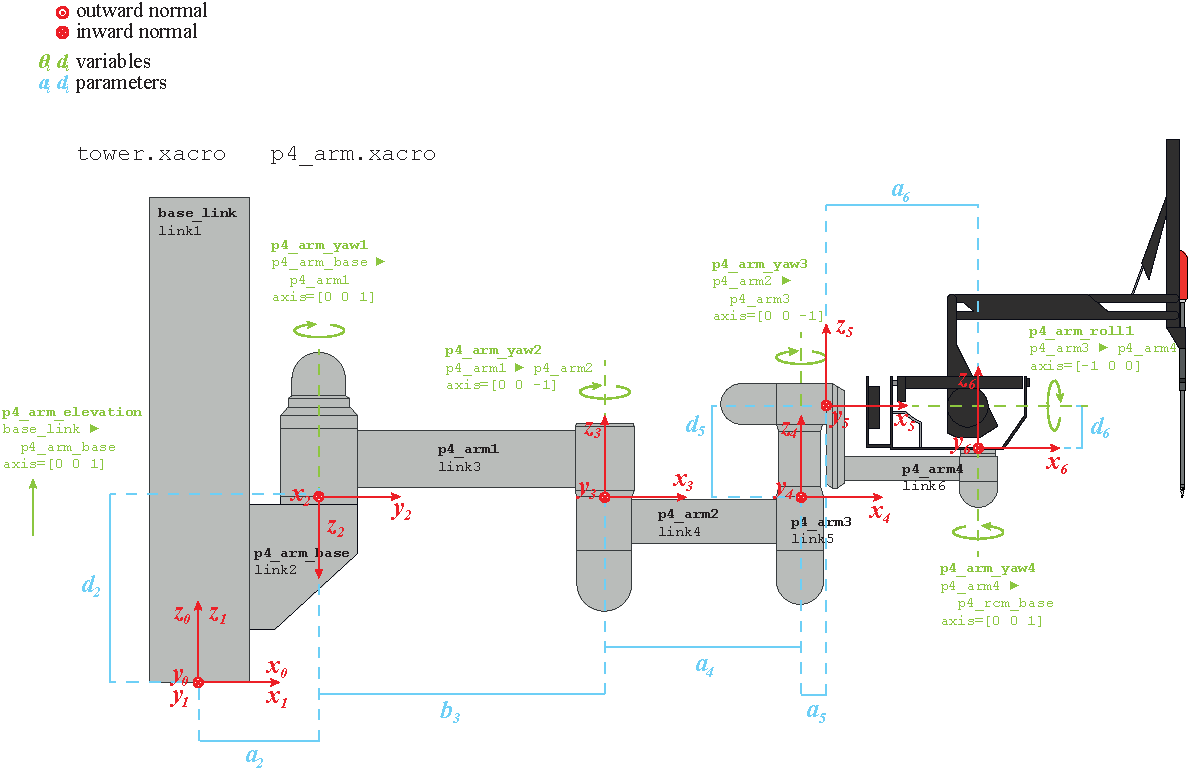
\includegraphics[width=\textwidth]{p4_arm_xacro_frames.pdf}\label{fig:p4_arm_xacro_frames}}%
	\vspace{1mm}
	\subbottom[Coordinate frames for the joints on the robot hand and instrument.]{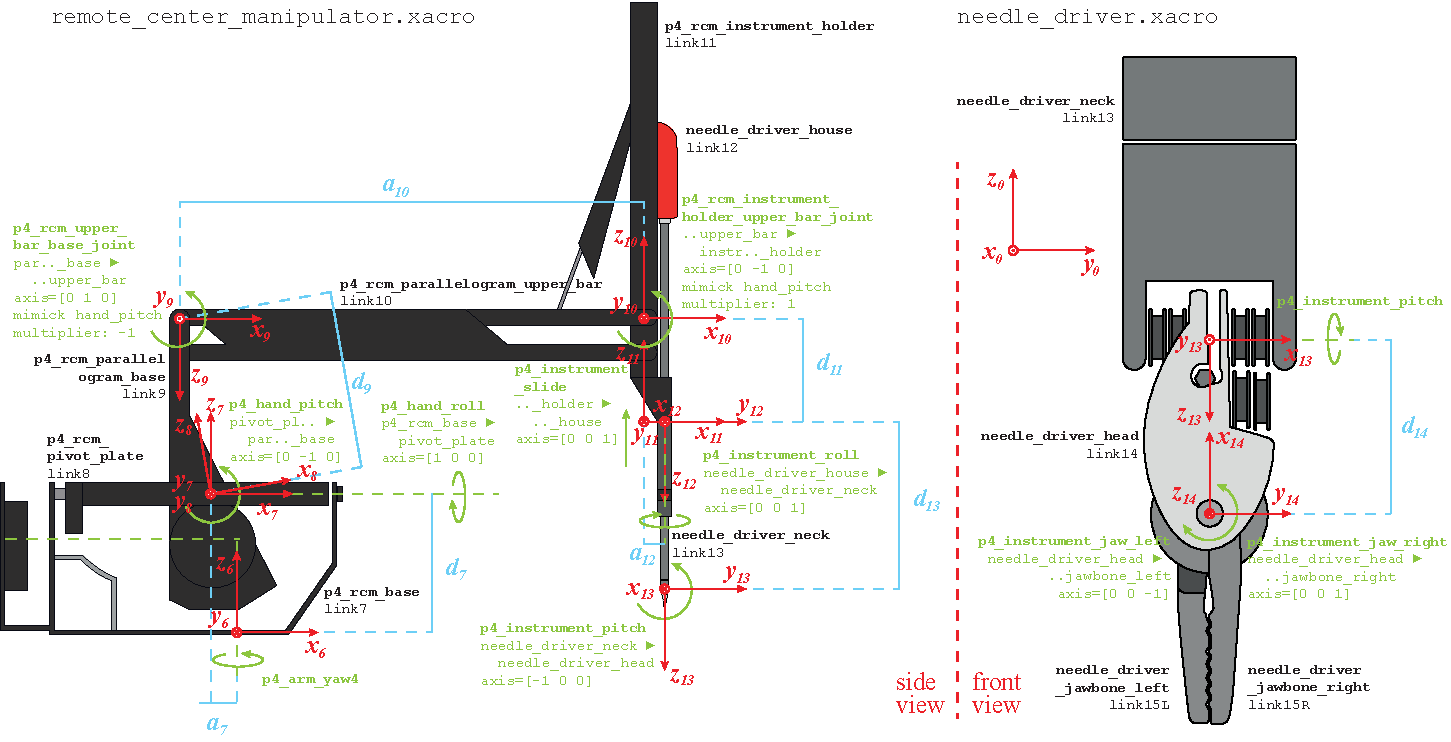
\includegraphics[width=1.1\textwidth]{p4_hand_xacro_frames.pdf}\label{fig:p4_hand_xacro_frames}}%
	\caption{Orientation and position of coordinate frames $\Psi_0$, $\Psi_b$, $\Psi_1$, ..., $\Psi_{14}$ according to the \gls{ros} \texttt{xacro} files.}
	\label{fig:robot_xacro_frames}
\end{figure}

The position and orientation of the $i$th coordinate frame is given as a transformation matrix from the $i-1$th frame, where fixed distances and rotations are measured along/about the axes of the $i-1$th frame while free distances and rotations are measured along/about the axes of the $i$th frame. The parameters and variables shown in \autoref{fig:robot_xacro_frames} are given in \autoref{tab:xacro_param}.

\begin{table}[htbp]
	\begin{tabular}{r | rrr c c l}
		frame  & $a$ [m] & $b$ [m] & $d$ [m] & fixed rot. $\alpha$ [rad] & free rot. $\theta$ [rad] & name\\\hline
		1 & 0 & 0 & $d_1^*$ & $I$ & $I$ & \texttt{elevation}\\
		2 & 0.186 & 0 & 0.554 & $R_z(\pi/2)R_x(\pi)$ & $R_z(\theta_2^*)$ & \texttt{arm\_yaw1} \\
		3 & 0 & 0.583 & 0 & $R_z(\pi/2)R_x(-\pi)$ & $R_z(-\theta_3^*)$ & \texttt{arm\_yaw2} \\
		4 & 0.479 & 0 & -0.001 & $I$ & $R_z(-\theta_4^*)$ & \texttt{arm\_yaw3} \\
		5 & 0.057 & 0 & 0.198 & $I$ & $R_x(-\theta_5^*)$ & \texttt{arm\_roll1} \\
		6 & 0.352 & 0 & -0.117 & $I$ & $R_z(\theta_6^*)$ & \texttt{arm\_yaw4} \\
		7 & -0.042 & 0 & 0.161 & $I$ & $R_x(\theta_7^*)$ & \texttt{hand\_roll} \\
		8 & 0 & 0 & 0 & $R_y(-0.288)$ & $R_y(-\theta_8^*)$ & \texttt{hand\_pitch} \\
		9 & 0.011 & 0 & 0.186 & $R_y(0.288)R_x(\pi)$ & $R_y(-\theta_8)$ & \texttt{upper\_bar} \\
		10 & 0.520 & 0 & 0 & $R_x(\pi)$ & $R_y(-\theta_8)$ & \texttt{instrument\_holder} \\
		11 & 0 & 0 & -0.120 + $d_{11}^*$ & $I$ & $I$ & \texttt{instrument\_slide} \\
		12 & 0.052 & 0 & 0 & $R_z(\pi/2)R_x(\pi)$ & $R_z(\theta_{12}^*)$ & \texttt{instrument\_roll} \\
		13 & 0 & 0 & 0.177 & $I$ & $R_x(-\theta_{13}^*)$ & \texttt{instrument\_pitch} \\
		14L & 0 & 0 & 0.009 & $R_y(\pi/2)R_x(\pi/2)$ & $R_z(-\theta_{14L}^*)$ & \texttt{instrument\_jaw\_left} \\
		14R & 0 & 0 & 0.009 & $R_y(\pi/2)R_x(\pi/2)$ & $R_z(\theta_{14R}^*)$ & \texttt{instrument\_jaw\_right} \\
	\end{tabular}
	\caption{Variables (marked with $^*$) and parameters for the robot in \autoref{fig:robot_xacro_frames}. $I$ is the identity matrix (no rotation). Recent measures indicate that $d_2=0.812$, $a_2=0.198$, $a_4=0.435$, $\alpha_8=R_y(-0.07)$, $\alpha_9=R_y(0.07)R_x(\pi)$, $a_9=0$ and $d_\text{11,fixed}=0.188$ ($\Rightarrow$ $d_{12}=0.472$).}
	\label{tab:xacro_param}
\end{table}


I.e. according to \autoref{tab:xacro_param}, the transformation between frame 1 and 2 is given as:
\begin{equation}
^1_2H = 
\begin{bmatrix}
R_z(\pi/2)R_x(\pi)R_z(\theta_2^*) & p_2\\
0 & 1
\end{bmatrix}, \qquad\qquad
p_2 = [0.186 \quad 0 \quad 0.554]^T
\end{equation}

The physical, low level controller and \gls{ros} limits for each of the variables are given in \autoref{tab:var_limits}


\begin{table}[htbp]
\small%
%\hspace{-10mm}
%\begin{tabular}{l | cccccc}
%limits & $d_1^*$ & $\theta_2^*$ & $\theta_3^*$ & $\theta_4^*$ & $\theta_5^*$ & $\theta_6^*$ \\\hline
%physical & & & & & & \\
%\texttt{xacro} & [0, 1] & $\pm\pi/2$ & $\pm 2.8$ & $\pm 2.8$ & $\pm\pi/2$ & $\pm 2.8$
%\end{tabular}\\\\%
%\vspace{1mm}\\%
\begin{tabular}{l | ccccccc}
limits & $\theta_7^*$ & $\theta_8^*$ & $d_{11}^*$ & $\theta_{12}^*$ & $\theta_{13}^*$ & $\theta_{14L}^*$ & $\theta_{14R}^*$ \\\hline
physical & $\pm$1.670 & [-0.951, 0.912] & [0.169, 0.410] & $\pm$4.712 & [-1.466, 1.536] & [-1.850, $\theta_{14R}^*$] & [$\theta_{14L}^*$, 1.702] \\
FPGA & [-1.333, 1.424] & [-0.812, 0.773] & [0.170, 0.409] & [-4.294, 4.416] & [-0.977, 0.908] & [-0.785, 1.335] & \\
\texttt{xacro} & $\pm\pi/2$ & [-0.8, 1] & $\pm$0.12 & $\pm3\pi/2$ & $\pm 1.5$ & $\pm 1.8$ & $\pm 1.8$
\end{tabular}
\normalsize
\caption{Limits on the (controllable) variables in \autoref{tab:xacro_param} and \autoref{fig:robot_xacro_frames}. The low level controller limits in the FPGA are set to avoid the physical limits, by switching off the motors on violation. The physical limits are measured limits.}
\label{tab:var_limits}
\end{table}

The first 6 degrees of freedom are elevation and rotation of the arm joints, and are manually set preoperatively and fixed, hence only the last 7 variables are controllable for trajectory planning. 
The frames are superimposed on the robot in \autoref{fig:robot_frames_pot}.

\vspace{-10mm}
\begin{figure}[htbp]
	\centering
\subbottom[Robot arm.]{\includegraphics[width=0.6\textwidth]{20150316_125233_red.pdf}\label{20150316_125233_red}}%
\hspace{5mm}
\subbottom[Robot arm.]{\includegraphics[width=0.25\textwidth]{20150316_125701_red.pdf}\label{20150316_125701_red}}%
\hspace{3mm}
\subbottom[Robot hand.]{\includegraphics[height=68mm]{20150316_140845_red.pdf}\label{20150316_140845_red}}%
\hspace{3mm}
\subbottom[Instr.]{\includegraphics[height=68mm]{20150317_110019_red.pdf}\label{20150317_110019_red}}%
\hspace{3mm}
\subbottom[Instr.]{\includegraphics[height=68mm]{20150317_111908_red.pdf}\label{20150317_111908_red}}%
\caption{Coordinate frame placement, distances and positive rotation direction for the robot arm, hand and instrument. In \autoref{20150316_125701_red} the positive rotation direction is shown for both ROS (green) and potentiometers (blue).}
\label{fig:robot_frames_pot}
\end{figure}

The position of the potentiometers measuring the joint variables 1-6 can be read from the interface to the secondary \gls{rio} as voltages. The scaling factor from these potentiometer voltages to the joint angle (in radians) are found through measurements and are given in \autoref{tab:arm_pot_factors}.
\vspace{2mm}
\begin{table}[H]
	\centering
\begin{tabular}{l | ccccc}
joint rotation [rad] & $\theta_2$, \texttt{yaw1} & $\theta_3$, \texttt{yaw2} & $\theta_4$, \texttt{yaw3} & $\theta_5$, \texttt{roll1} & $\theta_6$, \texttt{yaw4} \\
scaling factor [rad/V] & -0.225365326 & 0.302076216 & -0.306198114 & -0.311665937 & -0.314159265
\end{tabular}
\caption{Factor from potentiometer voltage measurements to arm joint angles.}
\label{tab:arm_pot_factors}
\end{table}



\newpage

\subsection{Testing Existing Kinematics in Matlab}
The single-axis rotation matrices are defined according to \autoref{eq:RxRyRz}

\begin{lstlisting}[language=matlab]
function rotation = rot(axis,angle)
	if axis==1
		rotation = [1 0 0; 0 cos(angle) -sin(angle); 0 sin(angle) cos(angle)];
	elseif axis==2
		rotation = [cos(angle) 0 sin(angle); 0 1 0; -sin(angle) 0 cos(angle)];
	elseif axis==3
		rotation = [cos(angle) -sin(angle) 0; sin(angle) cos(angle) 0; 0 0 1];
	end
end
\end{lstlisting}

The parameters are set according to \autoref{tab:xacro_param} (corrected according to measurements, see \autoref{tab:arm_pot_factors}) and the transformation matrices are computed as follows

\begin{lstlisting}[language=matlab]
%% Existing reference frames according to xacro files

% parameters: distances [m], a: along x, b: along y, d: along z
a = [0.0 0.198 0.0 0.435 0.057 0.352 -0.052 0.0 0.0 0.430 0.0 0.052 0.0 0.0 0.0];
b = [0 0 0.583 0 0 0 0 0 0 0 0 0 0 0 0];
d = [0 0.812 0 -0.001 0.198 -0.117 0.161 0 0.186 0 -0.104 0.0 0.177 0.009 0.009];

% parameters: rotations [rad]
R = [eye(3) rot(3,pi/2)*rot(1,pi) rot(3,pi/2)*rot(1,-pi) eye(3) eye(3) eye(3) eye(3) rot(2,-0.1745) rot(2,0.1745)*rot(1,pi) rot(1,pi) eye(3) rot(3,pi/2)*rot(1,pi) eye(3) rot(2,pi/2)*rot(1,pi/2) rot(2,pi/2)*rot(1,pi/2)];
for i = 1:length(a)
	Rot(:,:,i) = R(:,(i-1)*3+1:i*3);
end

% -------------------------------------------------------------------------
% variables: actuation axes
ax = [3 3 -3 -3 -1 3 1 -2 2 -2 3 3 -1 -3 3];

% first make the variable rotation matrices (assume all variables are angles)
for i = 1:length(a)
	Rot_var(:,:,i) = rot(abs(ax(i)),sign(ax(i))*state(i));
end
% eliminating the two rotations where the variable is a distance
Rot_var(:,:,1) = eye(3);
Rot_var(:,:,11) = eye(3);

% making the variable translation vectors
for i = 1:length(a)
	for j = 1:3
		if i == 1 || i == 11
			if j == abs(ax(i)) 
				p(j,i) = sign(ax(i))*state(i);
			end
		else
			p(j,i) = 0;
		end
	end
end

% Transformation matrices (forward kinematics)
for i = 1:length(a)
	fixed = [Rot(:,:,i) [a(i) b(i) d(i)]'; zeros(1,3) 1];
	free = [Rot_var(:,:,i) p(:,i); zeros(1,3) 1];
	Trans(:,:,i) = fixed*free;
end
\end{lstlisting}

Measurements of distances

\section{Defining Kinematics According to Denavit-Hartenberg Convention}

I order to simplify calculations, the robot coordinate frame convention Denavit-Hartenberg is adapted, and a 

The coordinate frames of the robot hand and instrument is shown in \autoref{fig:robot_frames}, and defined in the following.

%\begin{figure}[htbp]
%	\hspace{-10mm}
%	\subbottom[Coordinate frames for the joints on the robot "hand".]{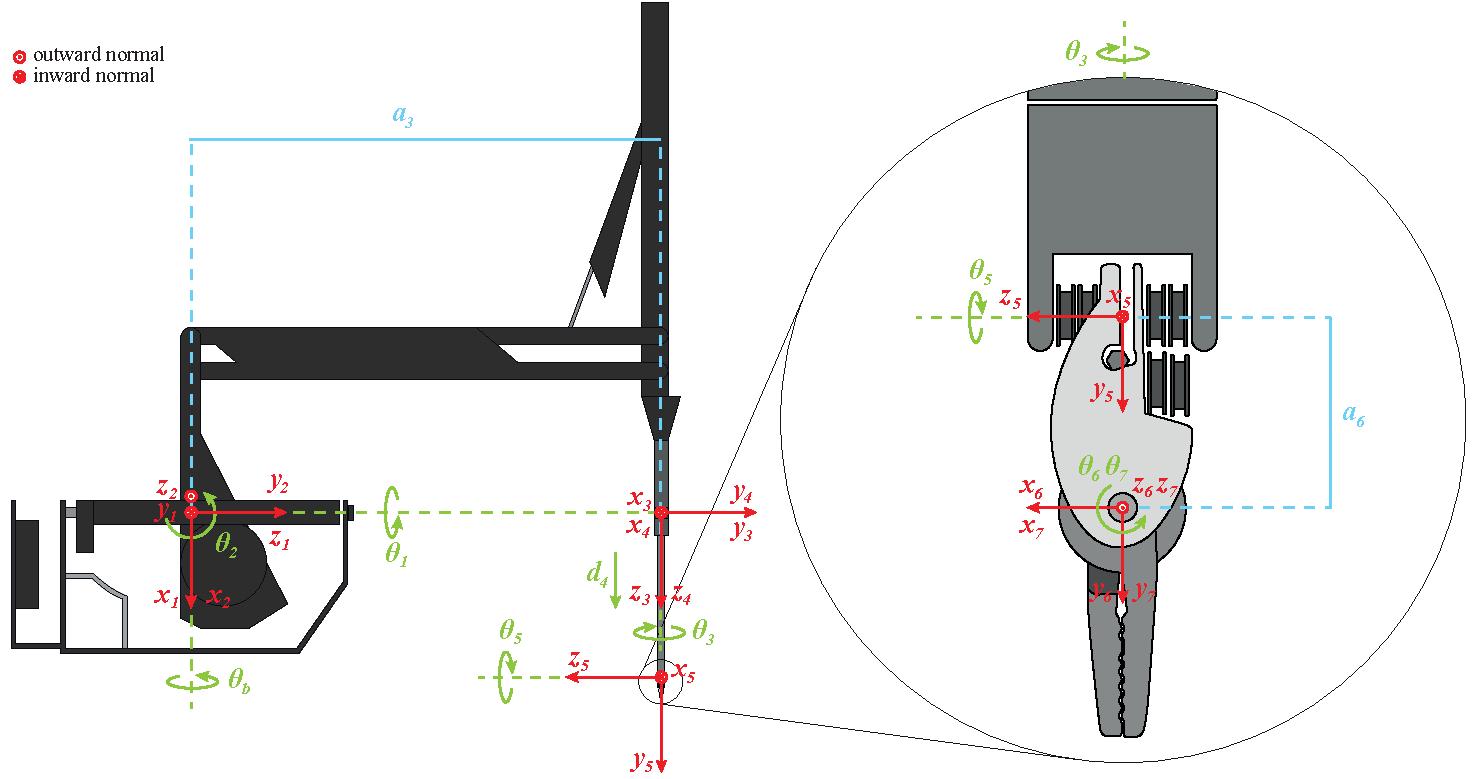
\includegraphics[width=1.2\textwidth]{robot_coordinate_systems_new.pdf}\label{fig:robot_coordinate_systems}}%
%	\vspace{1mm}
%	\subbottom[The\,\,da\,\,Vinci\,\,inertial\,\,frame.]{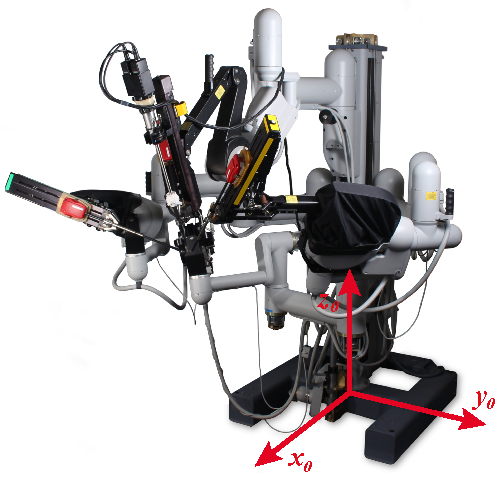
\includegraphics[height=5.1cm]{robot_base_frame1.pdf}\label{fig:robot_base_frame}}%
%	\hspace{10mm}
%	\subbottom[Robot arm (grey) with inertial and robot hand base frame.]{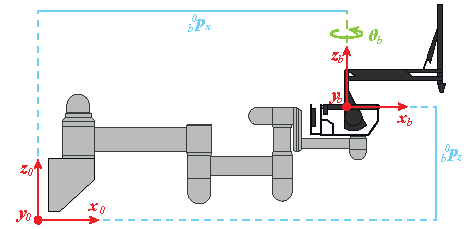
\includegraphics[height=4.7cm]{robot_arm_with_frames.pdf}\label{fig:robot_arm_with_frames}}%
%	\caption{Orientation and position of coordinate frames $\Psi_0$, $\Psi_b$, $\Psi_1$, ..., $\Psi_7$ relative to the da Vinci robot.}
%	\label{fig:robot_frames}
%\end{figure}

The inertial reference frame $\Psi_0$ is fixed with its origin at the robot base, as seen in \autoref{fig:robot_base_frame}. Assuming all arm joints (grey part of \autoref{fig:robot_arm_with_frames}) have zero angle, the configuration of the robot base frame (the joint of attachment between robot arm and robot hand) given in the inertial coordinates, is a pure translation along the inertial $x$- and $z$-axes:
\begin{equation}
^0_b T = \begin{bmatrix}
I & ^0_bp\\
0 & 1
\end{bmatrix}, 
\qquad\qquad\qquad
^0_bp = [^0_bp_x \quad 0 \quad ^0_bp_z]^T
\end{equation}

All rotating frames are defined such that they have rotation freedom $\theta$ about their $z$-axis, and all translating frames will translate along their $z$-axis. The rotation matrices $^a_bR$ consist of the free rotation about the $z$-axis and possibly a rotation of $\alpha=90^\circ$, to ensure that the rotation (or translation) freedom of each frame is about/along the frame's $z$-axis. The translation vectors $^a_bp$ may consist of a variable distance $d$ along the $z$-axis and a fixed distance $a$ between the frame origins.

The base link frame is rotated $\alpha=90^\circ$ about its $y$-axis to coincide with the first link frame $\Psi_1$ (see \autoref{fig:robot_coordinate_systems} and \ref{fig:robot_arm_with_frames}), and can according to \autoref{eq:RxRyRz} be expressed as
\begin{equation}
^b_1 T(\theta_1) = 
\begin{bmatrix}
R_y(\alpha) R_z(\theta_1) & 0\\
0 & 1
\end{bmatrix}
\end{equation}

The first link frame is rotated $\alpha=90^\circ$ about its $x$-axis to coincide with the second link frame $\Psi_2$ (see \autoref{fig:robot_coordinate_systems})
\begin{equation}
^1_2 T(\theta_2) = 
\begin{bmatrix}
R_x(\alpha) R_z(\theta_2) & 0\\
0 & 1
\end{bmatrix} 
\end{equation}

The second link frame is translated $a_3$ along its $y$-axis and rotated $\alpha=90^\circ$ about its $y$-axis to coincide with the instrument roll frame $\Psi_3$ (see \autoref{fig:robot_coordinate_systems})
\begin{equation}
^2_3 T(\theta_3) = 
\begin{bmatrix}
R_y(\alpha)R_z(\theta_3) & ^2_3p\\
0 & 1
\end{bmatrix}, 
\qquad\qquad\qquad
^2_3p = [0 \quad a_3 \quad 0]^T
\end{equation}

The instrument slide frame $\Psi_4$ has no rotation compared to the instrument roll frame, but includes the variable distance $d_4$ (see \autoref{fig:robot_coordinate_systems})
\begin{equation}
^3_4 T(d_4) = 
\begin{bmatrix}
I & ^3_4p\\
0 & 1
\end{bmatrix}, 
\qquad\qquad\qquad
^3_4p = [0 \quad 0 \quad d_4]^T
\end{equation}

The instrument pitch frame (wrist frame) $\Psi_5$ is obtained by rotating $\Psi_4$ by $\alpha=90^\circ$ about its $x$-axis (see \autoref{fig:robot_coordinate_systems})
\begin{equation}
^4_5 T(\theta_5) = 
\begin{bmatrix}
R_x(\alpha)R_z(\theta_5) & 0\\
0 & 1
\end{bmatrix}
\end{equation}

The instrument yaw right (gripper right) frame $\Psi_6$ is displaced $a_6$ along the $\Psi_5$ $y$-axis, and the frame is rotated $-\alpha=-90^\circ$ about the $y$-axis
\begin{equation}
^5_6 T(\theta_6) = 
\begin{bmatrix}
R_y(-\alpha)R_z(\theta_6) & ^5_6p\\
0 & 1
\end{bmatrix}, 
\qquad\qquad\qquad
^5_6p = [0 \quad a_6 \quad 0]^T
\end{equation}

Finally the instrument yaw left (gripper left) frame $\Psi_7$ is neither rotated nor translated relative to the $\Psi_6$ frame (except for the free rotation about the $z$-axis as for all other configurations)
\begin{equation}
^6_7 T(\theta_7) = 
\begin{bmatrix}
R_z(\theta_7) & 0\\
0 & 1
\end{bmatrix}
\end{equation}

The fixed distances are $a_3=530$\,mm and $a_6=14$\,mm, and the slider distance is $0\leq d_4 \leq 220$\,mm \textcolor{red}{check these and measure the $\theta$s} 


\section{Beating Heart Dynamic Model}
Illustration of heart model and description of kinematics and dynamics.
Quasi-periodic rigid 3D motion, combination of two periodic motions \cite{bib:heart_berkeley}. Frequencies assumed known from ECG and mechanical ventilator.

"The estimated components are then combined to predict future motion of the heart surface. This information, in turn, is used in the design of an explicit controller that stabilizes the relative motion of a surgical tool to a desired distance and orientation with respect to the heart surface."

"We then present a control law that uses the predicted motion to asymptotically stabilize the motion of the surgical tool to a desired distance and orientation with respect to the heart surface."

"To simplify the analysis and allow real-time prediction, we do not take the cause of the motion into consideration, and only consider the kinematics of a local area of interest on the heart surface."

"Fortunately, in this application, we have a reasonably good estimate of the phase1 and frequency of the two motion components: the respiratory phase and frequency can be obtained from the mechanical ventilator, and the cardiac phase and frequency are detected by an ECG monitor."

"choosing a convenient initial position and orientation for $\Psi_d$, e.g. such that $p^d_h(0)=0$ and $R^0_d(0) = I$

Relative configuration between heart and robot tool $H^h_r$ (with $R^h_r =[r_x, r_y, r_z]$) and error function $J(H^h_r)$
\begin{equation}
J(H^h_r) = \underbrace{\tfrac{1}{2}k_p (p^h_r-\Delta r_z)^T(p^h_r-\Delta r_z)}_\text{translational error} + \underbrace{k_x (1-e_x^T r_x) + k_y (1-e_y^T r_y) + k_z (1-e_z^T r_z)}_\text{rotational error}
\end{equation}
\begin{tabular}{rl}
	where &\\
	$\Delta$ & is the desired relative distance between the tool and the heart\\
	$E=[e_x,e_y,e_z]$ & is a rotation matrix describing the desired orientation of the tool frame\\
	$k_p,k_x,k_y,k_z$ & are constant positive parameters\\
\end{tabular}\\

Then $J$ is equal to zero (has its minimum) only when $p^h_r=\Delta r_z$ (the origin of $\Psi_r$ given in h coordinates is $\Delta$ away from the origin of $Psi_h$ along the surface normal) and $R^h_r=E$ (frame h and r axes are aligned).
\begin{align}
\dot{J} &= 
\begin{bmatrix}
k_x \hat{e}_x r_x + k_y \hat{e}_y r_y + k_z \hat{e}_z r_z\\
k_p(p^h_r - \Delta r_z)
\end{bmatrix}^T
\begin{bmatrix}
\omega^{h,h}_r \\
r^{h,h}_r
\end{bmatrix}
= (dJ)^T T^{h,h}_r\\
\dot{H}^h_r &= 
\begin{bmatrix}
\hat{\omega}^{h,h}_r r_x & \hat{\omega}^{h,h}_r r_y & \hat{\omega}^{h,h}_r r_z & \hat{\omega}^{h,h}_r p^h_r + v^{h,h}_r\\
0 & 0 & 0 & 0
\end{bmatrix}\\
(\dot{dJ}) &=
\begin{bmatrix}
-k_x \hat{e}_x \hat{r}_x  - k_y \hat{e}_y \hat{r}_y - k_z \hat{e}_z \hat{r}_z & 0\\
-k_p(\hat{p}^h_r - \Delta \hat{r}_z) & k_p I
\end{bmatrix}
T^{h,h}_r
\end{align}

"We do not consider specific robot dynamics at this point and only specify the desired inertial acceleration $\dot{T}^{0,0}_r$ of the robot end effector frame $\Psi_r$. Proposed desired acceleration"
\begin{equation}
\left(\dot{T}^{0,0}_r\right)_\text{des} = \dot{T}^{0,0}_h - \text{Ad}_{H^0_h} K_1 (\dot{dJ}) + \text{ad}_{T^{0,0}_h} T^{0,h}_r - \text{Ad}_{H^0_h} K_2 (T^{h,h}_r + K_1 dJ)
\end{equation}
\begin{tabular}{rl}
	where & \\
	$K1, K_2$ & are symmetric and positive definite matrices\\
	$H^0_h$ & is the estimated configuration of the frame $\Psi_h$ at the area of interest on the heart surface\\
	$T^{0,0}_h$ & is the estimated velocity of the frame $\Psi_h$ at the area of interest on the heart surface\\
	$\dot{T}^{0,0}_h$ & is the estimated acceleration of the frame $\Psi_h$ at the area of interest on the heart surface\\
\end{tabular}\\

This controller drives $T^{h,h}_r$ to $-K_1dJ$ by the gain $K_2$, along the steepest descend of $J$. Asymptotic stability at $J=0$, with Lyapunov function
\begin{equation}
V=\kappa_1 J + \tfrac{1}{2} (T^{h,h}_r + K_1dJ)^T K_2^{-1}(T^{h,h}_r + K_1dJ)
\end{equation}
\begin{tabular}{rl}
	where & \\
	$\kappa_1$ & is a positive constant strictly less than 4 times the smallest singular value of $K_1$, $0<\kappa_1 <4\sigma_\text{min}(K_1)$
\end{tabular}

Assuming the robot achieves perfect tracking of $\left(\dot{T}^{0,0}_r\right)_\text{des}$, the time derivative of $V$ along the system trajectories is
\begin{equation}
\dot{V} = -\left(T^{h,h}_r + (K_1 - \tfrac{\kappa_1}{2}I)dJ\right)^T \left(T^{h,h}_r + (K_1 - \tfrac{\kappa_1}{2}I)dJ\right) - \kappa_1(dJ ^T(K_1 - \tfrac{\kappa_1}{4}I)dJ
\end{equation}
\begin{tabular}{rl}
	where & \\
	$I$ & is the identity matrix\\
	$K_1 - \tfrac{\kappa_1}{4}$ & is strictly positive because of the choice of $\kappa_1$\\
\end{tabular}

\chapter{Dynamic Model of a Beating Heart}\label{app:dynamic_model_heart}
The relative velocity of two frames, meaning both the linear and angular velocity, can be concisely expressed as a 4x4 matrix (a twist) $T^{c,a}_b$, that describes the relative velocity of frame b with respect to b expressed in frame c
\begin{equation}
T^{c,a}_b = H^c_a \dot{H}^a_b H^b_c
\end{equation}

\chapter{SOSTOOLS Matlab Toolbox}\label{app:sostools}

As described in \citep{bib:sostools_manual}, an SOS program is initialized by declaring the independent variables as \texttt{syms} or \texttt{pvar} and optionally scalar decision variables as \texttt{syms}, and initializing an SOS program with the command \texttt{sosprogram} (in the below, grey denotes optional inputs)

\hspace*{1cm} \texttt{>> syms x1 dvar;}\\
\hspace*{1cm} \texttt{>> prog = sosprogram(x1\textcolor{grey}{,dvar});}

Now an SOS program called \texttt{prog} with the independent variable \texttt{x1} and the decision variable \texttt{dvar} has been initialized. An SOS variable \texttt{S} is added to the program by defining the monomial vector \texttt{Z} and calling the function \texttt{sossosvar}

\hspace*{1cm} \texttt{>> Z = monomials(x1,degrees);}\\
\hspace*{1cm} \texttt{>> [prog,S] = sossosvar(prog,Z);}

where \texttt{degrees} is the degrees of variables desired in the monomial; \texttt{[2 4]} would in this case give that \verb|Z = [x1^2; x1^4]| while \texttt{degrees = 0:2} would result in \verb|Z = [1; x1; x1^2]|. Declaring an SOS polynomial is done similarly to declaring an SOS variable

\hspace*{1cm} \texttt{>> Zp = monomials(x1,degrees);}\\
\hspace*{1cm} \texttt{>> [prog,P] = sospolyvar(prog,Zp);}

When all the necessary SOS variables and polynomials are defined, equalities (expression $=0$) and inequalities (expression $\geq 0$) can be defined for the program

\hspace*{1cm} \texttt{>> prog = soseq(prog,P-S);}\\
\hspace*{1cm} \texttt{>> prog = sosineq(prog,-diff(P,x1)-S);}

When all variables and constraints are input to the program, the solver is called with \texttt{sossolve}, which will return an overview of the precision of the solution (if any was found) as a residual error norm, number of iterations and time elapsed for solving the problem. To get the solution (coefficients) found for any of the SOS variables or polynomials, call the \texttt{sosgetsol}

\hspace*{1cm} \texttt{>> prog = sossolve(prog);}\\
\hspace*{1cm} \texttt{>> getB = sosgetsol(prog,P)}




If no solution could be found, the degree (and thereby complexity) of some SOS variables or polynomials may be increased through their monomials, which may yield a solution to the SOS problem.

In this and the following chapters, barrier certificates are attempted to be constructed by use of Putinar's Positivstellensatz in \autoref{def:putinar} with the Matlab toolbox SOSTOOLS (see \autoref{app:sostools} for a short introduction to the toolbox). In this chapter the first and second order systems depicted in \autoref{fig:stepresponseslide} are considered with a static reference on the position.

\section{Defining a Polynomial Barrier Certificate in SOSTOOLS}\label{sec:app_sostools_barrier_search}

A polynomial barrier certificate can be constructed using \gls{sos} optimization, e.g by using an \gls{sos} program such as SOSTOOLS, which is a convex relaxation framework based on sum of squares decompositions of multivariate polynomials and semidefinite programming solvers \citep{bib:prajna_framework}. A short introduction to the SOSTOOLS syntax is presented in \autoref{app:sostools}.
Searching for a barrier certificate in SOSTOOLS require the definition of all of the vaiables and polynomials given by \autoref{eq:barrier_constraints_putinar} as follows:

\renewcommand{\labelitemii}{$\circ$}
\renewcommand{\labelitemiii}{$\bullet$}
\begin{itemize}
	\itemsep-0.5mm
	\item \textbf{Initialize the Program}\\
	First declare the state space variables $x\in\mathbb{R}^n$ as \texttt{syms} or \texttt{pvar}, and initialize the SOS program with the system states by the function \texttt{sosprogram}.
	\item \textbf{Define the Vector Field}\\
	The open-loop state space system $f_{ol}(x)$ is defined, and a controller is found according to pole placement or another preferred method. Then write the closed-loop system equation $f_{cl}$ in terms of the symbolic state vector.
	\item \textbf{Set up the Constraints on the Polynomial Barrier Certificate}\\
	Declare a monomial vector $Z_B$ in $x$ (or part of $x$) of sufficiently large degree, and parametrize the polynomial $B(x)$ as a function of $Z_B$ with \texttt{sospolyvar}.  
	The problem of finding the coefficients for the barrier certificate is now for each region $\mathcal{X}$, $\mathcal{X}_u$ and $\mathcal{X}_0$ a matter of defining the following:
	\vspace*{-1mm}
	\begin{itemize}
		\item \textbf{Define the Polynomials $g_j(x)$}\\
		Define one or more polynomials $g_j$ that are positive in the region to be defined and negative outside. Each polynomial may be solely a function of the robot tool position (and velocity) for static boundaries, and also a function of the heart position (and velocity) for dynamic boundaries. 
		\item \textbf{Declare the SOS Variables $q_j(x)$}\\
		Declare monomial vectors $Z_{q_j}$ in $x$ of appropriate degree (preferably as small as possible to keep the complexity of the problem as low as possible), and parametrize the SOS polynomials (multipliers) $q_j$ with \texttt{sossosvar}.
		\item \textbf{Set up the Inequality}\\
		Cf. the nonnegativity of an \gls{sos} polynomial ($q_0$), the \texttt{sosineq} can be written as the right-hand side of \autoref{eq:putinar_sos}: Choose a small positive number $\epsilon$ for defining the region $\mathcal{X}_u$;
		set up the inequality (corresponding to the region to be defined) according to \autoref{eq:barrier_constraints_putinar}. The inequality pertaining to a set may be defined in terms of several $g_j$s; if the set is defined by
		\begin{itemize}
			\item $g_1 \bigcap g_2 \bigcap ... \bigcap g_m$, then write $h - \sum q_jg_j\geq 0$
			\item $g_1 \bigcup g_2 \bigcup ... \bigcup g_m$, then write $h - q_1g_1\geq 0$, $h - q_2g_2\geq 0$ etc.
		\end{itemize} 
		Note that each expression in the inequalities of \autoref{eq:barrier_constraints_putinar} must have even degrees in the leading and trailing terms in order for the equality in \autoref{eq:putinar_sos} to hold.
	\end{itemize}
	\item \textbf{Solve the SOS Program}\\
	With all inequalities defined in the program, SOSTOOLS is now ready to solve for the barrier certificate with \texttt{sossolve}, if any certificate exists for the given system $f_{cl}(x)$. If no solution is found, increasing the degree of the \gls{sos} variables $q_j$ or the polynomial $B(x)$ may yield a solution. Otherwise it can be concluded that safety cannot be guaranteed of the closed-loop system under scrutiny. 
\end{itemize}





\textcolor{red}{Matter of defining degree of B and qs - how to decide?}
In the following section an example is given on how to search for a barrier certificate with SOSTOOLS.








%\textcolor{red}{Og hvordan bruger I så det. Kør eksemplet videre, så det er klart hvordan (8.2e) oversættes til SOS program. Jeg synes I skal køre eksemplet hele vejen igennem og idregne det i SOSTOOLS. På denne måde overbeviser i læseren og, at I kan oversætte teorien til praktisk implementation - Og dette giver points! }



\subsection{Example of Barrier Certificate Search with SOSTOOLS}
This section presents a simple example of a barrier certificate search for a 1D first order state space system with $x_1\in\mathcal{X}\subset\mathbb{R}$ corresponding to the robot slide joint being the only degree of freedom (see \autoref{fig:safe:overview} for an overview of the slide movement). First the system is defined, and a controller is designed with pole placement.
\begin{lstlisting}[language=matlab]
% Define state-space system with x1 = robot position
tau = 0.11; % time constant for the robot slide
A = -1/tau;
B = 1/tau;
K = place(A,B,[-10*1/tau]);
\end{lstlisting}
Then the symbolic state variables are declared for the SOS program in SOSTOOLS with the command \texttt{pvar}, which corresponds to the command \texttt{syms} in the Matlab symbolic toolbox. Now the SOS program \texttt{prog} can be initialized using the function \texttt{sosprogram} which takes the state variable(s) as input. For a short introduction to SOSTOOLS and its syntax, see \autoref{app:sostools}.
\begin{lstlisting}[language=matlab]
% Declare state variables
pvar x1

% Initialize the sum of squares program
prog = sosprogram(x1);
\end{lstlisting}
%The reference for the robot position is generated as the 1D heart position, taking into account the system gain $\bar{N}$, and the closed-loop system equation is written as a function of the sybolic state. %\textcolor{red}{Something is wrong with the reference..?}
The vector field or derivative of the state can now be defined in terms on the symbolic state variable. This function is necessary for the SOS program when requiring that the Lie derivative of the barrier certificate must be negative on the set $\mathcal{X}$.
\begin{lstlisting}[language=matlab]
% Vector field dx/dt = fx (closed loop)
fx = (A-B*K)*x1;
\end{lstlisting}
For ease of defining a (1D) function $g$ that is positive on an interval [$p_1\,\,\, p_2$], a parabola function is used.
\begin{lstlisting}[language=matlab]
function [a,b,c] = parabola(p1,p2)
a = -1;
b = a*(p1^2-p2^2)/(p2-p1);
c = -a*p1^2-b*p1;
end
\end{lstlisting}
Now declare the polynomial barrier function with the command \texttt{sospolyvar}. To do this, a monomial vector must be specified with \texttt{monomials} (see the monomial example in \autoref{eq:monomial_example}), which takes as input the state variable(s) and the monomial degree(s). The monomial degrees for $B(x)$ are chosen as low as possible until a solution can be found. In this case a solution can be found for a degree of $B(x)$ that is 0:4.
\begin{lstlisting}[language=matlab]
% Declare polynomial barrier function
zB = monomials(x1,0:4);
[prog,Bx] = sospolyvar(prog,zB);
\end{lstlisting}
Now the region $\mathcal{X}$ can be defined for the slide region $\pm0.1$\,m using the Lie derivative inequality in \autoref{cer3_putinar}, which is defined with the command \texttt{sosineq}. The SOS polynomials $q$ are of the form in \autoref{eq:sos_polynomial} and are declared with the command \texttt{sossosvar}, also taking a monomial vector as input.
\begin{lstlisting}[language=matlab]
% Define space X in R^n
[a,b,c] = parabola(-0.1,0.1); % get coefficients for parabola which is positive for x in [-0.1,0.1]
gX = a*x1^2+b*x1+c;
zX = monomials(vars,0:2);
[prog,qX] = sossosvar(prog,zX);
prog = sosineq(prog,-diff(Bx,x1)*fx-gX*qX);
\end{lstlisting}
Similarly, the region $\mathcal{X}_u$ is defined according to the SOS inequality in \autoref{cer2_putinar} as the area between slide positions 5-10\,cm.
\begin{lstlisting}[language=matlab]
% Define space Xu in X
[a,b,c]=parabola(0.05,0.1);
gXu = a*x1^2+b*x1+c;
zXu = monomials(x1,0:2);
[prog,fXu] = sossosvar(prog,zXu);
prog = sosineq(prog,Bx-gXu*fXu);
\end{lstlisting}
And finally the region $\mathcal{X}_0$ is defined according to the SOS inequality in \autoref{cer1_putinar} as $\mathcal{X}\setminus\mathcal{X}_u$.
\begin{lstlisting}[language=matlab]
% Define space X0 in X
[a,b,c] = parabola(-0.1,0.05);
gX0 = a*x1^2+b*x1+c;
zX0 = monomials(x1,0:2);
[prog,fX0] = sossosvar(prog,zX0);
prog = sosineq(prog,-Bx-gX0*fX0);
\end{lstlisting}
With all three areas defined according to \autoref{eq:barrier_constraints_putinar}, the program is ready to be solved by using the command \texttt{sossolve}. If a solution is found, an overview of the solution accuracy is printed in the Matlab terminal as the residual norm, number of iteration steps and solving time. To get the polynomial $B(x)$ use the function \texttt{sosgetsol}.
\begin{lstlisting}[language=matlab]
% Solve for B
prog = sossolve(prog);
getB = sosgetsol(prog,Bx)
\end{lstlisting}
For this particular program, the solution barrier certificate is found to be
\begin{equation}
B(x) = 0.016168\cdot x_1^4 + 0.0064892\cdot x_1^3 + 0.00072547\cdot x_1^2 + 6.5473e\text{-}8\cdot x_1 - 2.7291e\text{-}6
\end{equation}
and is depicted in \autoref{fig:barrier_1storder_staticlim}.

\begin{figure}[htbp]
	\hspace*{-12mm}
	\includegraphics[width=1.1\textwidth]{1stordersys_staticlimits.pdf}
	\caption{A barrier certificate is found with SOSTOOLS that complies with the requirements in \autoref{eq:barrier_constraints}: it is positive on $\mathcal{X}_u=\{x_1\in [0.05,\,\,0.1]\}$ and negative on $\mathcal{X}_0=\{x_1\in [-0.1,\,\,0.05]\}$, and its Lie derivative is nonpositive on $\mathcal{X}=\{x_1\in [-0.1,\,\,0.1]\}$.}
	\label{fig:barrier_1storder_staticlim}
\end{figure}



\section{Safety Verification of First Order System}
First a linear open-loop state space system is defined according to the measurement of a step on the robot slide, showing a time constant $\tau=110$\,ms, giving the closed-loop system in \autoref{eq:1storder_1D_ss}:
\begin{equation}
\dot{x} = Ax+Bu = Ax+B(\bar{N}x_{ref}-Kx) = %-\tau^{-1}x+\tau^{-1}u=
-\tau^{-1}x+\tau^{-1}(\bar{N}x_{ref}-Kx)
\label{eq:1D_1storder}
\end{equation} 
which can be recast as the augmented state-space system
\begin{equation}
\dot{\tilde{x}}=
\dot{\begin{bmatrix}
	x_1\\x_{ref}
	\end{bmatrix}} =
\begin{bmatrix}
A-BK&B\bar{N}\\0&0
\end{bmatrix}
\begin{bmatrix}
x_1\\x_{ref}
\end{bmatrix}
= f_{cl}(x)
\label{eq:xtilde_1storder_1D}
\end{equation}
with no dynamics on the reference. A controller $K$ is found according to pole placement as described in \autoref{sec:K_Nbar_1D_1storder}, i.e. for the first order 1D system in \autoref{eq:1D_1storder} a controller that is 10 times faster than the system will be $K=9$. Similarly the system scaling factor $\bar{N}$ is determined according to the method described in \autoref{sec:K_Nbar_1D_1storder} as $\bar{N}=10$.
The independent state variables are defined and the SOS program initialized as described in \autoref{sec:app_sostools_barrier_search}.

%Now the $g_j$ functions in \autoref{eq:barrier_constraints_putinar} are constructed according to \autoref{fig:safe:overview}:
%\begin{itemize}
%%\itemsep-1.3mm
%\itemsep-0.7mm
%\item The set $\mathcal{X}$ is defined by constructing a (second order polynomial) function $g_{1}(x_1)\geq 0 \in [\Lambda_{\text{lim}-},\Lambda_{\text{lim}+}]= [-0.1,0.1]$\,m, delimiting the region of possible robot tool positions, and another function $g_2(x_{ref})\geq 0 \in [\Lambda_{h-}+\Delta,\Lambda_{h+}-\Delta]=[-0.1+\Delta,0.05-\Delta]$\,m, delimiting the region of allowable reference positions 
%\end{itemize}

The linear first order system from \autoref{eq:1storder_1D_ss} is defined with the same pole placement controller and thereby system gain as in \autoref{eq:K_1} and \ref{eq:barm_1}, and the same regions/intervals assigned for $\mathcal{X}$, $\mathcal{X}_u$ and $\mathcal{X}_0$ as given in \autoref{fig:safe:overview} - see \autoref{fig:intervals_for_sos}.
\begin{lstlisting}[language=matlab]
% 1D system WITH STATIC REFERENCE
clear all; clc; 

% Time constant from measurement
tau = 0.11;
% State-space matrices from first order open-loop system
A = -1/tau;
B = 1/tau;
% Setpoint controller that is xx times faster than the system
xx = 10;
K = place(A,B,[xx*A]);

C = 1;
D = 0;
Acl = A-B*K;
sysol = ss(A,B,C,D);
syscl = ss(Acl,B,C,D);

% Internal gain in the system for compensation of the reference
Nbar = -inv(C*inv(A-B*K)*B+D);

% Set upper and lower limits for the set intervals X, Xu and X0
Xmax = 0.1;
Xmin = -0.1;
Xumax = Xmax;
Xumin = 0.05;
X0max = Xumin;
X0min = Xmin;
\end{lstlisting}

\begin{figure}[htbp]
	\centering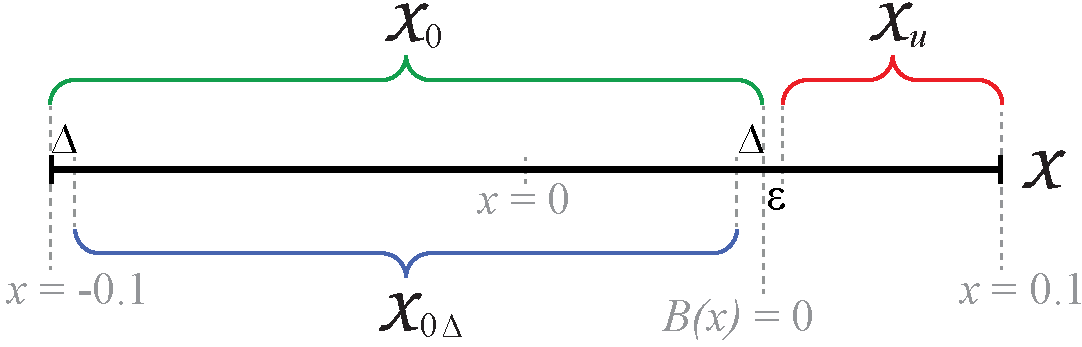
\includegraphics[width=0.6\textwidth]{intervals_for_sos.pdf}
	\caption{Intervals for the 1D case study, where the solid black line represents the interval $\mathcal{X}=\{x_1\in [-0.1, 0.1]\}$, and the interval $\mathcal{X}_0$ defines the interval where $B(x)\leq 0$, while $\mathcal{X}_u$ defines the interval where $B(x)>0$, separated from the zero level set by the small distance $\epsilon$. The interval $\mathcal{X}_{0\Delta} \subset \mathcal{X}_0$ is the interval of positions from which a reference can be taken $x_{ref}\in\mathcal{X}_{0\Delta}$. This interval is slightly smaller than the safe initial set $\mathcal{X}_0$, separated from the zero level set of $B(x)$ by the small distance $\Delta$.}
	\label{fig:intervals_for_sos}
\end{figure}

The small $\epsilon>0$ from \autoref{cer2_putinar} is defined "as small as possible", and another small $\Delta>0$ is introduced in order to be test for validity of a controller with references within the interval $\mathcal{X}_{0\Delta} \subset \mathcal{X}_0$ with a distance of at least $\Delta$ to the zero level set of $B(x)$, see \autoref{fig:intervals_for_sos}.
\begin{lstlisting}[language=matlab]
% Distance reference should keep to the unsafe region
delta = 0.001;

% Distance which the unsafe region is allowed to deviate from the desired zero level set specified by the g(x) defining Xu
epsilon = 0.00001;
\end{lstlisting}
The SOS program is initialized with the augmented state $\tilde{x}$ and thereby vector field as defined in \autoref{eq:xtilde_1storder_1D}. 
\begin{lstlisting}[language=matlab]
% =============================================
% Control Barrier Function Search for 1D system WITH STATIC REFERENCE
pvar x1 xref
xtilde = [x1; xref];

% =============================================
% First, initialize the sum of squares program
prog = sosprogram(xtilde);

% =============================================
% Vector field dt/dx = fx (closed loop)
fx = [A-B*K B*Nbar; 0 0]*xtilde;
\end{lstlisting}
The polynomial $B(x)$ is declared in as small degree "as possible". If any odd-order functions $g_j$ exist, $B(x)$'s leading term should be of an even degree higher than the uneven degree of the leading term of that $g_jq_j$. \textcolor{red}{It is considered that $B(x)$ should only be a function of the position and not of the reference, as the controller is considered as a static position setpoint controller for one single reference, and the program then tests the set of controllers, each with a setpoint within the interval $\mathcal{X}_{0\Delta} \subset \mathcal{X}_0$, for safety.}
\begin{lstlisting}[language=matlab]
% =============================================
% Declare polynomial degree of barrier function (FUNCTION OF BOTH X1 AND XREF?)
zB = monomials(x1,0:4);
[prog,Bar] = sospolyvar(prog,zB);
\end{lstlisting}
As $B(x)$ should be valid for the set $\mathcal{X}$, $\mathcal{X}$ is defined by $g_1(x_1)$ being positive on the slide interval, \textcolor{red}{and simultaneously $g_2(x_{ref})$ being positive on the interval $\mathcal{X}_{0\Delta} \subset \mathcal{X}_0$.} See \autoref{fig:intervals_for_sos} and \ref{fig:1D_static_gfunctions}.

\begin{figure}[htbp]
	\hspace*{-5mm}
	\subbottom[The $g(x_1)$ functions defining the sets $\mathcal{X}$, $\mathcal{X}_u$ and $\mathcal{X}_0$.]{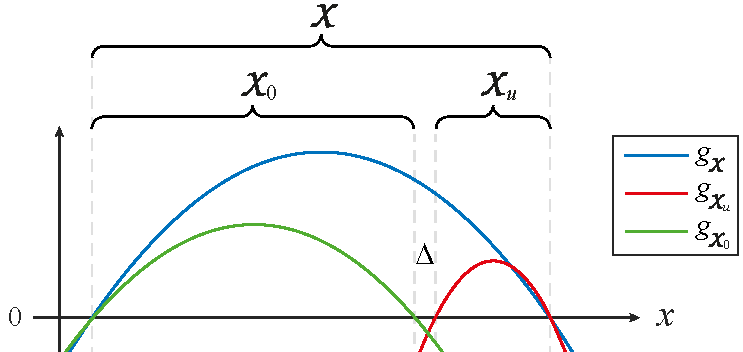
\includegraphics[width=0.55\textwidth]{1stordersys_staticlimits_g.pdf}\label{fig:1stordersys_staticlimits_g}}%
	\hspace{-2mm}
	\subbottom[The function $g(x_{ref})$ also used to define $\mathcal{X}$.]{\includegraphics[width=0.55\textwidth]{1stordersys_staticlimits_gref.pdf}\label{fig:1stordersys_staticlimits_gref}}%
	\caption{The functions $g$ used to define the sets $\mathcal{X}$, $\mathcal{X}_u$ and $\mathcal{X}_0$ by the interval in which they are positive, i.e. $\mathcal{X}_u$ is defined by the interval where $g_{X_u}(x_1)$ is positive in \autoref{fig:1stordersys_staticlimits_g}. In the definition of the set $\mathcal{X}$, corresponding to the space where the barrier certificate is valid, also a function $g$ of the reference/setpoint is used. This means that the barrier certificate is valid for all controllers with setpoint within the interval where $g(x_{ref})$ is positive.}
	\label{fig:1D_static_gfunctions}
\end{figure}

\begin{lstlisting}[language=matlab]
% =============================================
% Define space X in Rn

% Define g1(x1) to be positive on the region that we want X to encompass
[a,b,c]=parabola(Xmin,Xmax); % get coefficients for parabola
gX1 = a*x1^2+b*x1+c;

% Declare SOS polynomials q1(xtilde) in the full state (CHOICE OF DEGREEE?)
zX1 = monomials(xtilde,0:2); 
[prog,qX1] = sossosvar(prog,zX1);

% With g2(xref) define X only on the interval of allowed references
[a,b,c]=parabola(X0min+delta,X0max-delta);
gX2 = a*xref^2+b*xref+c;

% Declare SOS polynomials q2(xtilde) (CHOICE OF DEGREE?)
zX2 = monomials(xtilde,0:2);
[prog,qX2] = sossosvar(prog,zX2);

% Setup SOS inequality according to Putinar's Positivstellensatz
prog = sosineq(prog,-[diff(Bar,x1) diff(Bar,xref)]*fx-gX1*qX1-gX2*qX2);
\end{lstlisting}
The unsafe set is defined as the interval where the position $x_1$ takes values between 5 and 10\,cm, see \autoref{fig:intervals_for_sos} and \ref{fig:1D_static_gfunctions}. \textcolor{red}{It is not clear whether also the reference should be part of the definition of $\mathcal{X}_u$ (with a $g_2(x_{ref})$ positive on the same interval as $g_1(x_1)$), it has been tested both with and without, but there is no clear indication from the results that is should or should not be included.}
\begin{lstlisting}[language=matlab]
% =============================================
% Define space Xu in X

% Define g1(x1) to be positive on the region that we want Xu to encompass
[a,b,c]=parabola(Xumin,Xumax);
gXu1 = a*x1^2+b*x1+c;

% Declare SOS polynomials q1(xtilde) in the full state (CHOICE OF DEGREEE?)
zXu1 = monomials(xtilde,0:3);
[prog,qXu1] = sossosvar(prog,zXu1);

% With g2(xref) define Xu outside the interval of allowed references
[a,b,c]=parabola(Xumin,Xumax);
gXu2 = a*xref^2+b*xref+c;

% Declare SOS polynomials q2(xtilde) (CHOICE OF DEGREE?)
zXu2 = monomials(xtilde,0:3);
[prog,qXu2] = sossosvar(prog,zXu2);

% Setup SOS inequality according to Putinar's Positivstellensatz
prog = sosineq(prog,Bar-epsilon-gXu1*qXu1);%-gXu2*qXu2);
\end{lstlisting}
\textcolor{red}{The same is the case for the definition of $\mathcal{X}_0$; it is defined as the safe position region, and it has been tested with and without the requirement of references in the interval $\mathcal{X}_{0\Delta} \subset \mathcal{X}_0$.}
\begin{lstlisting}[language=matlab]
% =============================================
% Define space X0 in X

% Define g1(x1) to be positive on the region that we want X0 to encompass
[a,b,c]=parabola(X0min,X0max);
gX01 = a*x1^2+b*x1+c;

% Declare SOS polynomials q1(xtilde) in the full state (CHOICE OF DEGREEE?)
zX01 = monomials(xtilde,0:4);
[prog,qX01] = sossosvar(prog,zX01);

% With g2(xref) define X0 only on the interval of allowed references
[a,b,c]=parabola(X0min+delta,X0max-delta);
gX02 = a*xref^2+b*xref+c;

% Declare SOS polynomials q2(xtilde) (CHOICE OF DEGREE?)
zX02 = monomials(xtilde,0:3);
[prog,qX02] = sossosvar(prog,zX02);

% Setup SOS inequality according to Putinar's Positivstellensatz
prog = sosineq(prog,-Bar-gX01*qX01);%-gX02*qX02);
\end{lstlisting}
In most cases the solution found has a leading term coefficient of order between -4 and -2, but very often the value of $B(x)$ is either positive or negative on the entire interval [-0.1,0.1]. \textcolor{red}{Strangely, in all tested combinations, $L_{f_{cl}}B(x)$ is positive-valued on an interval approximately [-0.02,0]. This and the fact that the zero level set of the barrier in no case is in $x=0.05$ makes it seem like we still haven't formulated the problem correctly in terms of the SOS description. We could use a little help to see what we do wrong.} 
\begin{lstlisting}[language=matlab]
% =============================================
% Solve for B
prog = sossolve(prog);
getB = sosgetsol(prog,Bar)

dBdx = [diff(getB,x1) diff(getB,xref)]

% =============================================
% Plot B and LfclB
figure
subplot(1,2,1);
Bx = plotB(getB,[Xmin,Xmax],0);
subplot(1,2,2);
LfclB = plotLfclB(dBdx,A,B,C,D,K,Nbar,[Xmin,Xmax]);
\end{lstlisting}

\textcolor{red}{It has been tried tweaking the constants $\epsilon$ and $\Delta$ as well as testing with all the monomial degrees $Z_B$, $Z_{X1}$, $Z_{X2}$, $Z_{u1}$, ($Z_{u2}$), $Z_{01}$, ($Z_{02}$), in degrees 0:2, 0:3, 0:4, and in/excluding the constraints from $x_{ref}$ on $\mathcal{X}_u$ an $\mathcal{X}_0$, but in no case $B(x)$ attains a shape that remotely reflects the requirements (on $x_1$) for $\mathcal{X}_u$ an $\mathcal{X}_0$.}


\chapter{Measurement Logs}\label{app:meas}
\section{Step Response of Slide Position}
\begin{itemize}
\item Configure the ROS environment as described in \autoref{app:ros}, i.e. make sure all low level controllers are running, that \texttt{roscore}, the \texttt{davinci\_driver} and the \texttt{moveit\_group} interface is running.
\end{itemize}
Now, open two terminals and prepare both by typing:
\begin{itemize}
\item \texttt{ssh <user name>surgery-srv.lab.es.aau.dk} 
\item \texttt{cd <path to root of workspace>}
\item \texttt{source devel/setup.bash}.
\end{itemize}
\subsection*{First Terminal}
Type:

\hspace{1cm} \texttt{rosrun davinci\_moveit\_config MoveGroupInterfaceExecute}

This launches a \gls{ui}. Type \textbf{c} + \textbf{enter} to enter custom joint angle mode. 

SHOW EXAMPLE!!!! ????
\subsection*{Second Terminal}
By subscribing to the \texttt{joint\_state} topic (\texttt{rostopic echo joint\_states}), all information about the current states can be fetched from the sensors. An example of this is shown below.

\lstdefinestyle{DOS}
{
    backgroundcolor=\color{black},
    basicstyle=\scriptsize\color{green}\ttfamily
}
\begin{lstlisting}[style=DOS]
---
header: 
  seq: 4553
  stamp: 
    secs: 1428950592
    nsecs: 666452523
  frame_id: ''
name: ['p4_hand_pitch', 'p4_hand_roll', 'p4_instrument_jaw_left', 'p4_instrument_jaw_right', 'p4_instrument_pitch', 'p4_instrument_roll', 'p4_instrument_slide']
position: [-0.021504180505871773, 0.027300411835312843, 0.0006707065622322261, -0.00013414131535682827, 0.0012072718236595392, -0.0896063968539238, 1.055011398420902e-05]
velocity: [0.0, 0.0, 0.0, 0.0, 0.0, 0.0, 0.0]
effort: [-0.5, -0.5, -0.5, -0.5, -0.5, -0.5, -0.5]
---
\end{lstlisting}

For this test, it is more appropriate to merely publish the slide position, this can be done by:

\hspace{1cm}\texttt{rostopic echo joint\_states/position[6]}

Which gives an output as shown below.

\begin{lstlisting}[style=DOS]
---
8.20564400783e-06
---
8.20564400783e-06
---
8.20564400783e-06
---
\end{lstlisting}
Instead of leaving the output as a terminal output, the information is mapped to a \texttt{.txt} file with a suitable name, e.g:

\hspace{1cm} \texttt{rostopic echo joint\_states/position[6] > taus\_05cm\_1\_speedlimit\_100.txt}

Use the MATLAB script and the recorded measurement data found under the path \autoref{app:cd} under \texttt{matlab\_scripts/slide\_step/plot\_slide\_pos.m}, to plot the recorded slide position along with an estimated first and second order approximation. The step response is seen in \autoref{fig:stepresponseslideapp}.
\begin{figure}[H]
\center
\includegraphics[scale=0.5]{step_slide.eps}
\caption{Step response from 0\,mm to 5\,mm. Plot details and measurements can be found in \autoref{app:cd} as \texttt{matlab\_scripts/slide\_step/plot\_slide\_pos.m}}. 
\label{fig:stepresponseslideapp}
\end{figure}
The approximated second and first order system are found as...????

\chapter{MATLAB Implementation of a Safe Control System for Instrument Slide}\label{app:slide_implement_1}
\begin{lstlisting}[language=matlab]
close all;
clear; 
clc; 
format long;
hfile = matlab.desktop.editor.getAll;

model = 2; % 0 = both, 1 = first order model, 2 = second order model

%--- parabola coeficients for position constraints ---%
a = 16/9; b = 4/45; c = -2/225; 
%--- elliptic paraboloid  coeficients for position constraints ---%
x10 = 1/40; x20 = 0; a1 = -3/40; b1 = -10; c1 = 1; c2 = -1

if model == 0
    B = 2;
    B_ = 1;
else
    B = 1;
    B_ = 0;
end

vv = 0;
for v = 1:1:B
    if v == 1 && B_ == 1
        model = 1;
        fprintf('Simulating first order model..\n');
    elseif v == 2 && B_ == 1
        model = 2;
        fprintf('Simulating second order model..\n');
    end
    
if model == 2
    s = tf('s'); % prepare Laplace operator
    ts = (28-9)*1/50; % 5 percent settling time
    tr = 0.1; % rise time
    wn = 1.8/tr; % calculate natural frequency
    zeta = -1/(wn*ts)*log(0.02); % calculate the damping ratio
    H = wn^2/(s^2 + 2*zeta*wn*s + wn^2); % calculate transfer function
    num = wn^2; % Specify numarator
    den = [1 2*zeta*wn wn^2]; % specify denominator
    %[A,B,C,D] = tf2ss(num,den); % convert to state space system
    %sys = ss(A,B,C,D); % make a sys
    A = [0 1; -wn^2 -2*zeta*wn];
    B = [0 wn^2]';
    C = [1 0];
    D = 0;
    sys = ss(A,B,C,D)
    x(1,1) = 0 % initial state position
    x(2,1) = 0; % initial state velocity
    K = acker(sys.a,sys.b,[-40 -50]);
elseif model == 1
    tau = 0.110; % time constant
    a_sys = -1/tau; %
    b_sys = 1/tau; % sine wave frequency
    sys = ss(a_sys,b_sys,1,0);
    x(1,1) = 0; % initial state;
    K = acker(a_sys,b_sys,[10*eig(sys.a)]); % control gain   
end

kappa = 1;
Nbar = - inv(sys.c*inv(sys.a-sys.b*K)*sys.b); % ensure unity gain
scrsz = get(groot,'ScreenSize'); % get screen information

%--- Find epsilon ---%
x_epsilon = 0.04; % find epsilon from desired soft limit
epsilon = a*x_epsilon^2 + b*x_epsilon + c; % find epsilon
syms x0
softlims = solve(a*x0^2 + b*x0 + c == epsilon); % find soft limits
epsilon = abs(epsilon); % specify ep silon as a positive number

XREF = [0.02 0.09 -0.14 -0.02 0.045 0.01]; % simulation setpoints
%XREF = [0.025 1 0.0 -0.2 0.045 0.01]; % simulation setpoints
xref = XREF(1); % initial reference

f = 5000; Ts = 1/f; % sampling frequency
N = 1; % simulation time in seconds
fprintf('Simulation time: %d seconds\n', N)

i = (0:Ts:N); % make simulation resolution realistic
utilde = zeros(round(length(i)),1); % init utilde
Rplot(1) = 1; % init reference plot

for R = 1:length(i)
  REFS = 6;
  if R == round(length(i)/REFS)*1
      xref = XREF(2);
      Rplot(2) = R;
  elseif R == round(length(i)/REFS)*2
      xref = XREF(3);
      Rplot(3) = R;
  elseif R == round(length(i)/REFS)*3
      xref = XREF(4);
      Rplot(4) = R;
  elseif R == round(length(i)/REFS)*4
      xref = XREF(5);
      Rplot(5) = R;
  elseif R == round(length(i)/REFS)*5
      xref = XREF(6);
      Rplot(6) = R;
  end
  
  if 1
    if model == 2
      max_vel = 2;
      if x(2,R) > max_vel
          x(2,R) = max_vel;
      elseif x(2,R) < -max_vel
          x(2,R) = -max_vel;
      end
    end
  end
 
  %--- determine sigma  ---%
  y(1,R) = sys.c*x(:,R);
  
  if model == 1
      if (a*(x(1,R))^2 + b*(x(1,R)) + c) <= -epsilon
          sigma = 0;
      elseif ((a*(x(1,R)).^2 + b*(x(1,R)) + c) > -epsilon) && ...
             ((a*(x(1,R)).^2 + b*(x(1,R)) + c) <  0)
          sigma = -2*((a*(x(1,R)).^2 + b*(x(1,R)) + c)/epsilon).^3 - ...
                   3.*((a*(x(1,R)).^2 + b*(x(1,R)) + c)/epsilon ).^2 + 1;
      else
          sigma = 1;
      end
  elseif model == 2
      cbf = (a.*(x(1,R)).^2 + b.*x(1,R) + c);
      if cbf <= -epsilon
          sigma = 0;
      elseif (cbf > -epsilon) && (cbf < 0)
          if model == 1
              sigma = -2*((a*(x(1,R)).^2 + b*(x(1,R)) + c)/epsilon).^3 - ...
                       3.*((a*(x(1,R)).^2 + b*(x(1,R)) + c)/epsilon ).^2 + 1;
          elseif model == 2
              sigma = -2*((a*(x(1,R)).^2 + b*(x(1,R)) + c)/epsilon).^3 - ...
                       3.*((a*(x(1,R)).^2 + b*(x(1,R)) + c)/epsilon ).^2 + 1;
          end
      else
          sigma = 1;
      end 
  end

  if mod(R,1000) == 1 
      if R ~= 1
          fprintf('iter = %d of %d\n', R-1, length(i)-1);
      else
          fprintf('iter = %d of %d\n', R, length(i)-1);
      end
  end

  if model == 2
      LgB(1,R) = (c1*wn^2*(2*x(2,R) + 2*x20))/b1^2;
      LfB(1,R) = (c1*x(2,R)*(2*x(1,R) + 2*x10))/a1^2 - ...
          (c1*(2*x(2,R) + 2*x20)*(x(1,R)*wn^2 + 2*x(2,R)*zeta*wn))/b1^2;  
  elseif model == 1
      LgB(1,R) = (2*(a)*(x(:,R)) + (b))*(sys.b);
      LfB(1,R) = (2*(a)*(x(:,R)) + (b))*((sys.a)*x(:,R));
  end
  
  %-- Find controller by pole placement --%
  utilde(1,R) = xref*Nbar - K*x(:,R);

  %--- Find safe controller ---%
  threshold = 0.0001;
  gamma2 = 1;
  gamma1 = 0.5;
  if abs(LgB(1,R)) >= threshold
      k0(1,R) = -( ( LfB(1,R) + sqrt(LfB(1,R)^2 ...
          + kappa^2*LgB(1,R)*LgB(1,R)' )) /  (LgB(1,R)*LgB(1,R)')  ) *LgB(1,R);
      kplot(1,R) =  0;%k0(1,R);
  else
      k0(1,R) = x(1,R);
      kplot(1,R) = k0(1,R);
  end 
  
  u0(1,R) = sigma*k0(1,R)+(1-sigma)*utilde(1,R);
  
  if 1
    slide_lim = 0.1;
    if u0(1,R) > slide_lim
      u0(1,R) = slide_lim;
    elseif u0(1,R) < -slide_lim
      u0(1,R) = -slide_lim;
    end
  end
  
  LfclB(1,R) = LfB(1,R) + LgB(1,R).*k0(1,R);
  
  %--- Forward Euler ---%
  xdot = sys.a*x(:,R) + u0(1,R)*sys.b;
  x(:,R+1) = xdot*Ts + x(:,R);
  sig(1,R) = sigma;
  
end

%--- plot LfB(x) and LgB(x) ---%
M = 2.5;
figure('Position',[scrsz(1) scrsz(4) scrsz(3)/3 scrsz(4)/3])
hold on
plot(y(1,1:end),LfB(1,:),'-b','linewidth',1)
plot(y(1,1:end),LgB(1,:),'-g','linewidth',1)
x_p = find(LfB >= 0);
plot(y(x_p),LfB(x_p),'-r','linewidth',1)
plot([-0.11 0.11], [0 0], ':k')
plot([-b/(2*a) -b/(2*a)],[-M M],'-.m');
plot([0.04 0.04],[-M M],'-.r');
plot([0.05 0.05],[-M M],'-.r');
plot([-0.09 -0.09],[-M M],'-.r');
plot([-0.1 -0.1],[-M M],'-.r');
h_legend = legend({'$L_fB(x)<0$','$L_gB(x)$','$L_fB(x) \geq 0$','zero level'}...
    ,'Interpreter','latex','location','northeast');
hold off
set(h_legend,'FontSize',14);
ax = gca;
%ax.YLim = [-M M];
ax.XLim = [-0.11 0.11];
fig = gcf;
fig.Name = 'Lie derivatives';
xlabel('slide position [m]')
ylabel('$L_fB(x) \, \wedge \, L_gB(x)$','Interpreter','latex')
set(gca,'fontsize',14)
title('Lie derivatives', 'FontSize', 14);
if 1
    if  model == 1
        str1 = 'CBF extremity','Interpreter','latex';
        text(-b/(2*a),-1,str1);
    end
    str1 = '\Lambda_{s+}','Interpreter','latex';
    text(0.04,-1,str1);
    str1 = '\Lambda_{h+}','Interpreter','latex';
    text(0.05,-1,str1);
    str1 = '\Lambda_{s,}','Interpreter','latex';
    text(-0.09,-1,str1); 
    str1 = '\Lambda_{h-}','Interpreter','latex';
    text(-0.1,-1,str1); 
end
set(findall(gcf,'type','text'),'FontSize',14,'fontWeight','normal')
set(0,'defaultAxesFontName', 'Times New Roman')
set(0,'defaultTextFontName', 'Times New Roman')
box on


%--- plot Barrier function ---%
z = linspace(-1, 1, 10^4);
fprintf('plotting barrier function..\n')
figure('Position',[scrsz(1) scrsz(4)/10 scrsz(3)/3 scrsz(4)/3])
bar = a.*z.^2 + b.*z + c;
h0 = plot(z,bar,'-b', 'linewidth',1);
h0.DisplayName = 'barrier function';
hold on;
h1 = plot([-10 10],[0 0],'--k', 'linewidth', 1);
h1.DisplayName = 'zero line';
slide_lim_y = [-0.2 0.2]; 
slide_lim = [ 0.1  0.1];
h2 = plot(slide_lim, slide_lim_y, '-r', -slide_lim, slide_lim_y, '-r');
h2(1).DisplayName = 'slide limits';
plot(y(1,:),zeros(size(y)), 'xg')
plot(y(1,end),0, 'xk')
plot([x(1,end) x(1,end)], [-10 10], '-.r')
axis([-0.15 0.1 -0.015 0.02]);
grid off;
legend([h0, h1, h2(1)],...
        h0.DisplayName, h1.DisplayName, h2(1).DisplayName,...
       'Location', 'NorthEast');
fig = gcf;
fig.Name = 'Overview';
hold off;

%--- plot control signal ---%
fprintf('plotting control signals..\n')
figure('Position',[scrsz(1)*scrsz(4)/1.5 scrsz(4) scrsz(3)/5 scrsz(4)/2.8])
hold on
if vv == 1
    plot(linspace(0,length(i),length(u01(1,:))), u01(1,:),'-.r');
end
plot(linspace(0,length(i),length(u0(1,:))), u0(1,:),'-b');
fig = gcf;
fig.Name = 'control signal';
if vv == 1
    legend('control signal based on 1st order model','control signal based on 2nd order model')
else
    legend('control signal')
end
h_legend = legend({'$u(x),\,\,\,\,  \kappa = 1$'},'Interpreter','latex');
set(h_legend,'FontSize',14);
ax = gca;
fig = gcf;
%ax.XLim = [0 1000];
fig.Name = 'Control signals';
xlabel('time [s/1000]')
ylabel('u(x)')
set(gca,'fontsize',14)
title('Control signal', 'FontSize', 14);
box on
hold off

%--- plot state trajectory with boundaries ---%
fprintf('plotting states..\n')
figure('Position',[scrsz(1)*scrsz(4)*1.1 scrsz(4)/10 scrsz(3)/3 scrsz(4)/3])
hold on
plot(linspace(0,length(i),length(y(1,:))), y(1,:),'-b','linewidth',1);
plot(linspace(0,length(i),length(sig(1,:))), sig(1,:)./10,'-','Color',...
    [0/255,255/255,0/255],'linewidth',1);
if vv == 1
   plot(linspace(0,length(i),length(y1(1,:))), y1(1,:),'-.b','linewidth',1);
   plot(linspace(0,length(i),length(sig1(1,:))), sig1(1,:)./10,'-.','Color',...
        [0/255,255/255,0/255],'linewidth',1);
end
plot([0 length(i)], [-0.1 -0.1],'-r')
plot([0 length(i)], [softlims(1) softlims(1)],'-.r')
plot([0 length(i)], [-0.1 -0.1],':k')
Rplot(length(XREF) + 1) = length(i);
for j = 1:length(XREF)
    plot([Rplot(j) Rplot(j+1)],[XREF(j) XREF(j)],'-k', 'linewidth',1);
    plot(Rplot(j), XREF(j), '*k');
end
plot([0 length(i)], [softlims(2) softlims(2)],'-.r')
plot([0 length(i)], [0.05 0.05],'-r')
plot([0 length(i)], [0.1 0.1],':k')
h_legend = legend({'slide position','$\sigma(x)\cdot0.1$','$\Lambda_{h\pm}$','$\Lambda_{s\pm}$',...
    'physical limit','reference level'},'Interpreter','latex','location','southeast');
set(h_legend,'FontSize',14);
ax = gca;
ax.YLim = [-0.15 0.11];
ax.XLim = [0 length(i)];
fig = gcf;
fig.Name = 'states';
xlabel('time [s/1000]')
ylabel('slide position [m]')
set(gca,'fontsize',14)
if model == 1
    title('State trajectory for slide position based on first order model', 'FontSize', 14);
elseif model == 2
    title('State trajectory for slide position based on second order model', 'FontSize', 14);
end    
box on
hold off

if model == 2
    figure
    plot(x(2,:))
    title('velocity')
end
figure
plot(LfclB(1,:))
title('LfclB')


figure
hold on
plot(linspace(1,length(i),length(i)),LfB(1,:))
plot(linspace(1,length(i),length(i)),LgB(1,:))
hold off
legend('LfB','LgB')
title('LgB and LfB')


if model == 2
    figure
    plot(linspace(1,length(i),length(i)),((((x(1,1:end-1)+x10).^2))./a1^2 + ((x(2,1:end-1)+x20).^2)./b1^2)*c1 + c2)
    title('B(x1,x2)')
elseif model == 1
    figure
    plot(linspace(1,length(i),length(i)),a.*x(1,1:end-1).^2 + b.*x(1,1:end-1) + c)
    title('B(x1)')
end

end

if v == 1
    y1 = y(1,:);
    sig1 = sig(1,:);
    vv = 1;
    u01 = u0(1,:);
end

fprintf('Done!\n')
set(findall(gcf,'type','text'),'FontSize',14,'fontWeight','normal')
set(0,'defaultAxesFontName', 'Times New Roman')
set(0,'defaultTextFontName', 'Times New Roman')
\end{lstlisting}

\chapter{Attached CD}\label{app:cd}
\section*{$\bullet$ MATLAB scripts}
\section*{$\bullet$ Measurement Files}

\end{appendices}
\label{appendixend}

{\color{white}{\gls{lambdai}}}
{\color{white}{\gls{lambda}}}
{\color{white}{\gls{X}}}
{\color{white}{\gls{X0}}}
{\color{white}{\gls{Xu}}}
{\color{white}{\gls{lie2}}}
{\color{white}{\gls{A}}}
{\color{white}{\gls{B}}}
{\color{white}{\gls{C}}}
{\color{white}{\gls{D}}}
{\color{white}{\gls{q}}}

\end{document}